\documentclass[a4paper, 11pt]{article}

\usepackage{graphicx}
\usepackage[export]{adjustbox}
\usepackage[left=1in,right=1in,top=1in,bottom=1in]{geometry}
\usepackage{tcolorbox}
\tcbuselibrary{breakable}
\usepackage{xpatch}
\usepackage{xcolor}

\usepackage{marginnote}
\usepackage{enumitem}
\usepackage{caption}

\usepackage[bookmarksopen=true, 
				pdfauthor=Lubos Polerecky,
				pdftitle=Look@NanoSIMS,
				pdfsubject=User manual]{hyperref}

\linespread{1.2}

% LP commands
\newcommand{\ttt}[1]{\textsf{#1}}
\newcommand\ra{\rightarrow}
\newcommand\figref[0]{\textbf{Figure}}
\newcounter{step}
\setcounter{step}{0}
\newcommand\bul{\noindent$\bullet${ }}
\newcommand\bb[1]{\textbf{#1}}

% load more definitions and latex options
% define colors
\definecolor{lightgrey}{RGB}{240,240,240}
\definecolor{skyblue}{RGB}{135,206,250}
\definecolor{darkgold}{RGB}{120,75,4}
\definecolor{gold}{RGB}{239,191,4}
\definecolor{darkgreen}{RGB}{4,120,4}
\definecolor{darkblue}{RGB}{4,4,190}
\definecolor{purple}{RGB}{128,0,128}

% modify spacing around items
\setlist[itemize]{
	topsep=0pt plus 2pt minus 4pt,
	parsep=1pt plus 1pt, 
	itemsep=1pt plus 1pt}
\setlist[enumerate]{
	leftmargin=15pt, 
	topsep=2pt plus 2pt minus 4pt, 
	parsep=4pt plus 1pt, 
	itemsep=1pt plus 1pt}

% define appearance of figure caption and reference
\captionsetup{font={small,sl}, labelfont={small,bf,sl}}
\renewcommand{\thefigure}{\textbf{\arabic{section}.\arabic{figure}}}
\hypersetup{colorlinks=true,linkcolor=purple,urlcolor=purple}

%%% define boxes

% lans function box
\newcommand{\lans}[1]{\tcbox[nobeforeafter,
	tcbox raise base,
	%colback=lightgrey,
	%colframe=lightgrey,
	colback=gray!15, 
	colframe=gray!15,
	coltext=black,
	fontupper=\sf,
	left=0mm, right=0mm, top=0mm, bottom=0mm, 
	boxsep=0.25mm, 
	arc=0mm]{#1}}

% lans checkbox box
\newcommand{\lanscb}[1]{\tcbox[nobeforeafter,
	tcbox raise base,
	%colback=darkgreen!15,
	%colframe=darkgreen!15,
	colback=darkgreen!15,
	colframe=darkgreen!15,
	coltext=black,
	fontupper=\sf,
	left=0mm, right=0mm, top=0mm, bottom=0mm, 
	boxsep=0.25mm, 
	arc=0mm]{#1}}

% lans textfield box
\newcommand{\lanstf}[1]{\tcbox[nobeforeafter,
	tcbox raise base,
	colback=cyan!15,
	colframe=cyan!15,
	coltext=black,
	fontupper=\sf,
	left=0mm, right=0mm, top=0mm, bottom=0mm, 
	boxsep=0.25mm, 
	arc=0mm]{#1}}

% step box
\newcommand\stepbox[1]{%
	\vskip0.2\baselineskip
	\marginnote{\tcbox[nobeforeafter,
	tcbox raise base,
	colback=gold!20,
	colframe=gold!20,
      	fontupper=\footnotesize,
	left=1mm, right=1mm, top=1mm, bottom=1mm, 
	boxsep=0mm, 
	arc=0mm]{#1}}\noindent}
\newcommand\s{\addtocounter{step}{1}	\stepbox{Step~\thestep}}

% note box
\newcommand\nb{%
       \vskip0.5\baselineskip
	\marginnote{\tcbox[nobeforeafter,
	tcbox raise base,
	colback=purple!20,
	colframe=purple!20,
      	fontupper=\footnotesize,
	left=1mm, right=1mm, top=1mm, bottom=1mm, 
	boxsep=0mm, 
	arc=0mm]{Notes}}\noindent}

% section box:
\xpatchcmd{\section}{\normalfont\Large\bfseries}{\sectionbox}{}{\PatchFailed}
\newcommand*{\sectionbox}[1]{%	
	\begin{tcolorbox}[
	colback=purple!100,% background
	colframe=purple!100,% frame colour
	coltext=white, % text color
      width=\linewidth,%
      halign=left,
      valign=center,
      fontupper=\large\bfseries,
      arc=1mm, %auto outer arc,
    	boxrule=0mm,%
    	boxsep=.15\baselineskip,%
    	rounded corners,%
    	left*=0pt,%
    	right*=0pt,%
    	grow to right by=0.5\baselineskip,%
    	grow to left by=0.5\baselineskip%
       ]{#1}
	\end{tcolorbox} 
} %

% subsection box:
\xpatchcmd{\subsection}{\normalfont\large\bfseries}{\subsectionbox}{}{\PatchFailed}
\newcommand*{\subsectionbox}[1]{%
	\begin{tcolorbox}[
	colback=gold!70,% background
       colframe=gold!70,% frame colour
       coltext=black, % text color
       width=\linewidth,%
       halign=left,
       valign=center,
       fontupper=\large\bfseries,
       arc=1mm, auto outer arc,
    	boxrule=0mm,%
    	boxsep=.15\baselineskip,%
    	rounded corners,%
   	left*=0pt,%
    	right*=0pt,%
    	grow to right by=0.5\baselineskip,%
    	grow to left by=0.5\baselineskip%
       ]{#1}
	\end{tcolorbox} 
} %

% skyblue box
\newcommand{\skybluebox}[1]{%
\begin{tcolorbox}[
	colback=skyblue!10, 
	coltext=black, coltitle=black,
	colframe=skyblue!70,
	grow to right by=0.5\baselineskip,
	grow to left by=0.5\baselineskip,
    	rounded corners,%
   	left*=0pt,%
    	right*=0pt,%
	fonttitle=\bfseries,
	boxsep=1mm,
	title=#1]}

% gold box
\newcommand{\goldbox}[1]{%
\begin{tcolorbox}[
	colback=gold!10, 
	coltext=black, coltitle=black,
	colframe=gold!70,
    	rounded corners,%
   	left*=0pt,%
    	right*=0pt,%
	grow to right by=0.5\baselineskip,
	grow to left by=0.5\baselineskip,
	fonttitle=\bfseries,
	boxsep=1mm,
	title={#1}]}

% green box
\newcommand{\greenbox}[1]{%
\begin{tcolorbox}[
	colback=white, 
	coltext=black, coltitle=black,
	colframe=darkgreen!30,
	grow to right by=0.5\baselineskip,
	grow to left by=0.5\baselineskip,
    	rounded corners,%
   	left*=0pt,%
    	right*=0pt,%
	fonttitle=\bfseries,
	boxsep=1mm,
	title=#1]}

% graybox (gb)
\newcommand{\gb}{%
	\begin{tcolorbox}[%
	colback=lightgrey!10,%
    	colframe=lightgrey!50,%
    	boxrule=0mm,%
    	boxsep=.1\baselineskip,%
    	arc=1mm,%
    	rounded corners,%
    	breakable,%
    	left*=6pt,%
    	right*=6pt,%
    	boxsep=0mm,
	grow to right by=0\baselineskip,%
    	grow to left by=0.0\baselineskip%
	]}

% end of any tcolorbox
\newcommand{\tcbe}{\end{tcolorbox}}

% Title, author, date
\title{\LARGE \bf Look@NanoSIMS}
\author{{\large\bf by Lubos Polerecky}\\[6mm]
{\small Department of Earth Sciences, Utrecht University, Utrecht, The Netherlands (2013--today)} \\%[1mm]
{\small Max-Planck Institute for Marine Microbiology, Bremen, Germany (2002--2013)}\\[3mm]}
\date{User's manual, version 28-06-2025}

\begin{document}

\maketitle
\reversemarginpar 

\section*{Summary}
\textbf{Look@NanoSIMS}, or shortly \textbf{LANS}, is a program for processing and analysis of ion count image data produced by the NanoSIMS instrument. The original development of the program started back in 2008, but its active development continues until today based on input and requests from users (yes, it's more like a~long-term hobby). Although the program may be considered an `old school' in a number of aspects, it has matured well over the years. Once you get used to it, become aware of all of its features and figure out all the tricks, it allows you to analyze NanoSIMS data very thoroughly and efficiently. This document describes how to get started with the program and carry out such analyses from basic to advanced levels. 

\vskip6mm

\goldbox{Citation:}
Please use the following citation if you use Look@NanoSIMS:

\textsf{Polerecky et al.~(2012). Look@NanoSIMS --- a tool for the analysis of nanoSIMS data in environmental microbiology. \textit{Environmental Microbiology} 14 (4): 1009--1023.\\
DOI: 10.1111/j.1462-2920.2011.02681.x}
\tcbe

\vskip4mm

\skybluebox{Contact:}
If you have questions or want to provide feedback, you can contact the author via e-mail: 

\bul \ttt{L (dot) Polerecky (at) uu (dot) nl}

\vskip1mm\noindent You can also arrange a~video-conference meeting via Teams or Zoom if your questions are more difficult or you would like to collaborate on implementing a~new feature in Look@NanoSIMS.
\tcbe

\vskip4mm

\greenbox{Notation:}
Throughout this document, we will use text in coloured boxes when refering to a specific \lans{menu item} or \lans{action button}, \lanscb{checkbox} or \lanstf{text field} in the program's graphical user interface.
\tcbe

\newpage

\tableofcontents

\newpage

%%% Specify sections that should be included

%\section{Installation instructions}

LANS is a Matlab-based program. Thus, a \textbf{Matlab} installation is required to run LANS and execute its basic functions. This makes it possible to run LANS on a variety of operating systems, including Linux, Microsoft Windows and MacOS. However, this also limits LANS to users with access to a Matlab license. Additional functionality of LANS is achieved by integrating the program with \textbf{\LaTeX} (for exporting results in a nicely formatted PDF output) and data compression programs such as \textbf{zip} (for decompressing input files and compressing output generated by LANS), both of which are available for free.

%%

\subsection{Install Matlab}
\setcounter{step}{0}

\goldbox{}
Matlab is available from \url{www.mathworks.com} and requires a license. If you do not have a~personal license, it is useful to check whether your institution provides a~site-license that you can use (e.g., your university may have one for all students and academic staff). 
\tcbe

\sbx{Install the \bb{core} Matlab and two toolboxes: \bb{image processing toolbox} and \bb{statistics and machine learning toolbox}. }

\nbx{Matlab version R2024b is recommended to ensure that all LANS functions work as designed and presented in this document. LANS works with older Matlab versions as well (tested until R2019b), however, there is a~risk that some functions will issue errors due to less than perfect back-compatibility of Matlab. Presently, Matlab version 2025a or higher is \emph{not} recommended.}

\nnb{Some output generated by LANS, e.g., information generated during the alignment of planes and stored in the file \ttt{xyalign.mat}, may not be loaded correctly by an older Matlab version if it was generated by a~newer Matlab version. Thus, if you plan to use LANS in collaboration with other people, e.g., by sharing the files generated by LANS among each other, it is recommended that everyone in the team uses the same Matlab version.}

%%

\subsection{Install \LaTeX}
\setcounter{step}{0}

\goldbox{}
\LaTeX\ is required to enable export of graphical output as tagged PDF documents. 
\tcbe

\sbx{To install \LaTeX, use one of the well-established \LaTeX\ distributions for your operating system, as described on the \href{https://www.latex-project.org/get/}{\LaTeX\ project} website (e.g., \ttt{texlive} for Linux, \ttt{MikTeX} for Windows, \ttt{MacTex} for MacOS). Note that on-line LaTeX services, such as Overleaf, are insufficient; you really need a locally installed \LaTeX\ distribution.}
 
\sbx{To correctly integrate \LaTeX\ with LANS, check that the following executables and packages are installed and working:
 
\begin{itemize}
\item[--] executables: \ttt{epstopdf}, \ttt{pdflatex}
\item[--] packages: \ttt{graphicx}, \ttt{geometry}, \ttt{url}, \ttt{hyperref}, \ttt{adjustbox}
\end{itemize}}
 
\nbb{If you have never used \LaTeX\ on your computer, it may be that some \LaTeX\ packages, parti\-cu\-larly \ttt{geometry}, \ttt{hyperref} and \ttt{adjustbox}, are not installed during the `standard' installation steps. As a result, the execution of the LANS functions \lans{Export LaTeX and PDF output} (main LANS window) or \lans{Export images for each variable as PDF} (Process metafile window) may get \bb{stuck} if the packages are missing. If this happens, you need to fix this issue before you can continue with LANS in a~meaningful way. Appendix~A should give you some useful hints on how to do that.}

%%

\subsection{Install software for compressing/decompressing files}
\setcounter{step}{0}

\goldbox{}
This software is required for two main reasons:

\begin{enumerate}
 
\item It enables you to load compressed nanoSIMS datasets (\ttt{im.zip} files) by LANS. This is a~useful feature because \ttt{im.zip} files have roughly 5--10-fold smaller size than the original \ttt{im} files generated by the Cameca's nanoSIMS measurement software. It is recommended to store and distribute the raw data files by first compressing them with the \ttt{zip} program (extension \ttt{im.zip}). 

\item It allows you to compress the processed data generated by LANS. This is convenient for making data backups, since it is much more efficient to upload and download few compressed folders than hundreds of smaller files present in those folders.

\end{enumerate}
\tcbe

\sbx{If you work under Microsoft Windows, it is recommended to install \ttt{7-Zip} (freeware). If you work under Linux and MacOS systems, you do not need to do anything because \ttt{zip} and \ttt{unzip} are available by default.}

%%

\subsection{Install Look@NanoSIMS}
\setcounter{step}{0}

\goldbox{}
LANS is installed by simply copying the source files (\ttt{m} and \ttt{fig}) to a~folder on your computer.
\tcbe

\sbx{For convenience, the compressed file containing the \emph{latest version of LANS} is stored in this \href{https://www.dropbox.com/sh/gyss2uvv5ggu2vl/AABViAmt9WHryEP_xZBrCG_La?dl=0}{Dropbox folder}. Click on the \ttt{program} folder and then download the file \ttt{LANS-latest-src.zip}.}

\sbx{Unzip \ttt{LANS-latest-src.zip} to a folder of your choice.}

\sbx{Rename the \ttt{src} folder using a more reasonable name (e.g., \ttt{LANS-2025-07-27}, where the date refers to the LANS version).}

\nbx{In case the Dropbox link above does not work, because it became outdated or the official distribution location changed, visit the LANS github repository or try to search the internet for more updated information. For users familiar with git and github, LANS can be downloaded by pulling the source code from the \ttt{src} folder in the LANS github repository: \url{https://github.com/lpolerecky/LANS}.}

%%

\subsection{Starting LANS for the first time}
\setcounter{step}{0}

\goldbox{}
Before you run LANS for the first time, read through the content of the files \ttt{lookatnanosims.m} and \ttt{lans\_paths.m}, which can be found in the same location where you installed LANS. These two files contain important settings you need to adjust to reflect your specific local installation of LANS.  For example, you can specify there:
%\setlist{nolistsep}

\begin{itemize}%[noitemsep]
\item[--] locations of the compression/decompression software,
\item[--] location of the PDF viewer,
\item[--] default name of the file containing regions of interest (ROIs),
\item[--] default extension of the raw data files.
\end{itemize}
\tcbe

\nbx{If you browse through the LANS installation files, you will notice that the \ttt{*.fig} files, which define the graphical user interface (GUI), appear in two sub-folders: \ttt{figs} and \ttt{figs\_win}. This is required because GUI defined on Unix-like and Windows platforms do not look the same. This is an issue due to --- apparently --- limited cross-platform compatibility of Matlab visual objects. However, this issue is not important for you as an end-user of LANS. You only need to be aware of it. Should you wish to modify any of the \ttt{*.fig} files, you will need to modify those that correspond to your operating system.}

\nnb{Add examples of the relevant lines with the command lines.}

%%

\subsection{Starting LANS on a regular basis}
\setcounter{step}{0}
\vskip2.5mm

\sbx{Start Matlab.}

\sbx{Set the current folder to the folder where you installed LANS. You can do this through the menu or, more easily, entering one of the following commands in the Matlab console. 
\vskip1mm
\ttt{cd c:$\backslash$programs$\backslash$LANS}

\ttt{cd /home/your\_username/programs/LANS}
\vskip1mm
The precise syntax depends on whether you use Windows, Linux or MacOS, and on the path where you installed LANS. Thus, you will need to adapt it according to your local settings.}

\sbx{Once you are in the correct folder, enter the following command in the Matlab console:

\ttt{lookatnanosims}}

%%% place holder for LANS main gui
\begin{figure}[!t]
\centering
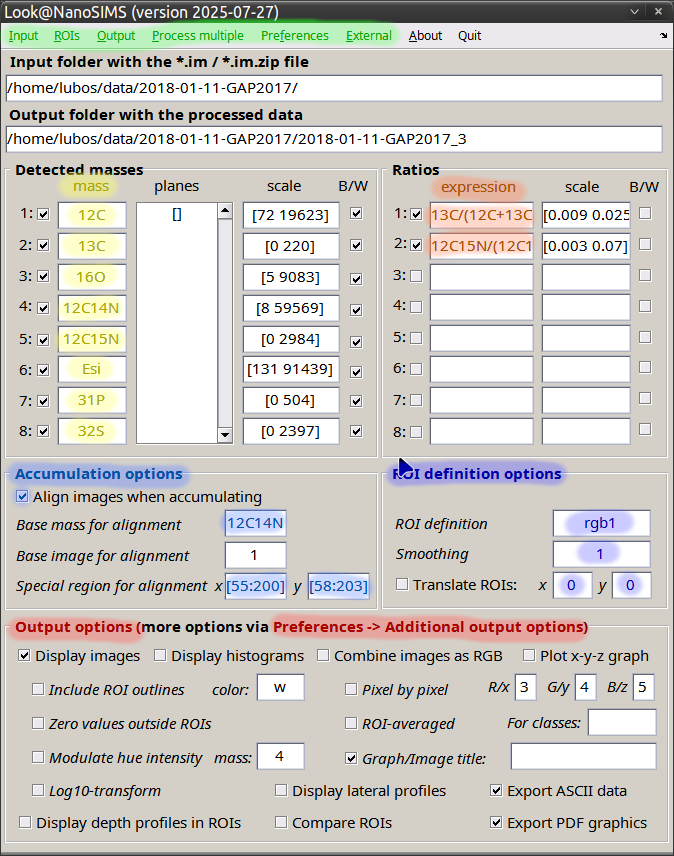
\includegraphics[scale=0.47]{figs1/LANS-maingui}
\caption{\label{fig1:mainLANSgui}%
Main window of the Look@NanoSIMS program.}
\end{figure}

\nbx{If everything is set up correctly, the main LANS graphical user interface (GUI) will open, as shown in Fig.~\ref{fig1:mainLANSgui}. You can start from there, as described in the following sections of this document.}

\nnb{During the data processing session, LANS provides quite a lot of useful information in the Matlab console. Thus, it is a good idea to \emph{always} keep an eye on the output in the console. You can do this by arranging your desktop such that both the LANS and Matlab console windows are visible at the same time. This is also useful in case you encounter an error while working in LANS. These errors will be shown in the console, too.}

%%

\subsection{Updating LANS}
\setcounter{step}{0}
\goldbox{}
{LANS is updated quite regularly. You can update it easily by entering in the Matlab console:
\ttt{lans\_webupdate}}
\tcbe

\nbx{You need to be in the folder where LANS is installed to run this command. In the process, you will be prompted to make a backup of your older LANS version, which is recommended to do, just in case.}

\nnb{If you are familiar with \ttt{git}, you can update LANS by pulling the latest sources from the LANS github repository \url{https://github.com/lpolerecky/LANS}.}

%\section{Organization of the input and output data}
\label{sec:data_organization}

\purplebox{}
Working with LANS, and with nanoSIMS data in general, can be a book-keeping challenge. To start with, you will have many raw data files (\ttt{im} or \ttt{im.zip} files) acquired at different dates and from different types of samples (e.g., different treatments). Additionally, processing of those raw data files with LANS will create many output files, including data in a~standard text format (files with extensions \ttt{dac}, \ttt{dat}, \ttt{txt}, or \ttt{tex}), matlab output (\ttt{mat} files), graphical output (\ttt{pdf}, \ttt{png} or \ttt{tif} files), and compressed folder back-ups (\ttt{zip} files). It is therefore a good idea to develop and maintain a~certain structure of those folders and output files, to \emph{keep everything organized}. 
\tcbe

In this document, we assume that the raw and processed nanoSIMS data are organized hierarchically as shown in Table~\ref{tab1:file_structure}. We have used this data organization at Utrecht University for many years, and it works pretty well. We therefore highly encourage users to adopt it as well. Its benefits will become more apparent later on, when we get to the point of explaining how to efficiently process and analyze \emph{multiple} nanoSIMS datasets from a particular project.

\begin{table}[!b]
\centering
\def\hsk{\hskip4mm}
\def\tsep{\hsk$\rightarrow$\hsk}
\caption{\label{tab1:file_structure} Hierarchical organization of the raw and processed nanoSIMS data implemented in LANS. A~more visual example of the data organization is shown in Fig.~\ref{fig2:data_organization}.}
\begin{tabular}{l@{\tsep}c@{\tsep}l@{\tsep}l@{\tsep}l}
\hline
\multicolumn{5}{l}{\bb{Folder organization from a project level to a dataset level:}}\\
\hline
root & project & measurment day 1 & raw dataset 1.1 & \color{red}{dataset folder} 1.1\\
\multicolumn{2}{c}{} & & raw dataset 1.2  & dataset folder 1.2\\
\multicolumn{2}{c}{} & & $\cdots$ & $\cdots$ \\
\multicolumn{1}{c}{} & & measurement day 2 & raw dataset 2.1  & dataset folder 2.1\\
\multicolumn{2}{c}{} & & raw dataset 2.2  & dataset folder 2.2\\
\multicolumn{2}{c}{} & & $\cdots$ & $\cdots$\\
\multicolumn{1}{c}{} & & $\cdots$ & $\cdots$ & $\cdots$\\
\hline
\multicolumn{5}{l}{\bb{Files and folder organization within a dataset level:}}\\
\hline
\multicolumn{2}{r}{\color{red}{dataset folder} $i$ $\rightarrow$} & \color{orange}{dat} & \multicolumn{2}{l}{\color{orange}{numbers in a text format}} \\
\multicolumn{2}{r}{$\rightarrow$} & \textcolor{darkgold}{pdf} & \multicolumn{2}{l}{\textcolor{darkgold}{images \&\ graphs in a pdf format}} \\
\multicolumn{2}{r}{$\rightarrow$} & \multicolumn{3}{l}{\hspace{-2mm}processing definition files (\textcolor{purple}{alignment, ROIs, preferences})} \\
\multicolumn{2}{r}{$\rightarrow$} & \multicolumn{3}{l}{\hspace{-2mm}\textcolor{purple}{OutputG.pdf (graphical output summary)}}\\
\hline
\end{tabular}
\end{table}

At the highest level of the data organization is a root folder that contains \emph{all} nanoSIMS data. This folder contains `project folders' with nanoSIMS data belonging to \emph{specific projects}. Each `project folder' contains `day folders' with data acquired on \emph{different measurement days}. Each `day folder' contains the actual \emph{raw datasets} (\ttt{im} or \ttt{im.zip} files). 

When a particular raw dataset is processed, the corresponding output is stored in a `dataset folder' with the \emph{same name} as the dataset. Each `dataset folder' contains sub-folders with the \emph{results} of the analysis, including numerical values such as ROI-specific ion counts or ion count ratios, stored in the sub-folder \ttt{dat}, and graphical output such as images or scatter plots, stored in the sub-folder \ttt{pdf}. The `dataset folder' also contains information defining the processing steps, such as alignment of planes, definition and classification of regions of interest (ROIs), and preferences. This information is useful if you want to go back to the analysis of the same dataset after you have analyzed a different one, e.g., to perform quality checks or more in-depth analyses. Finally, the `dataset folder' also contains a PDF file (\ttt{OutputG.pdf}) with a~comprehensive graphical summary of the analysis output. This file is useful if you wish to share the results for a specific dataset with project collaborators.

\begin{figure}[!hp]
\centering
\begin{tabular}{c@{\hskip1pt}c}
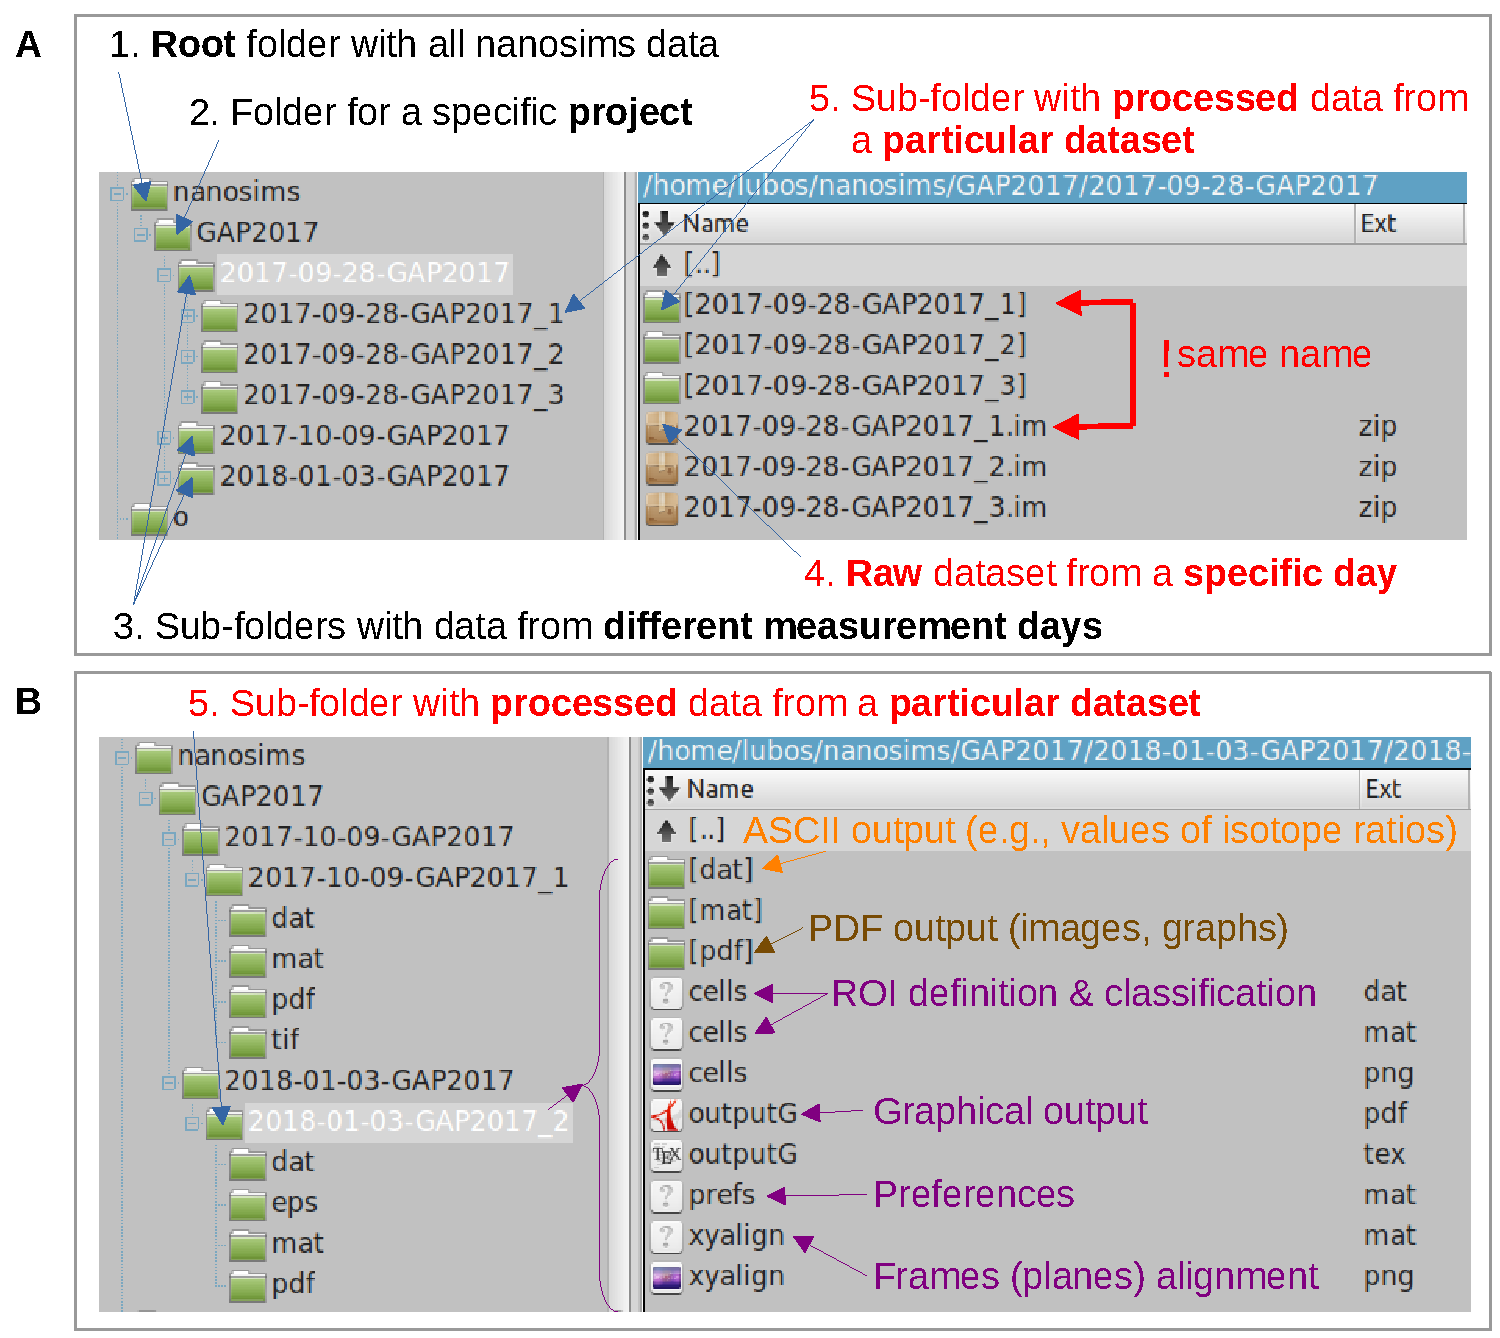
\includegraphics[width=0.485\textwidth,valign=t]{figs2/folders_organizationAB} 
&
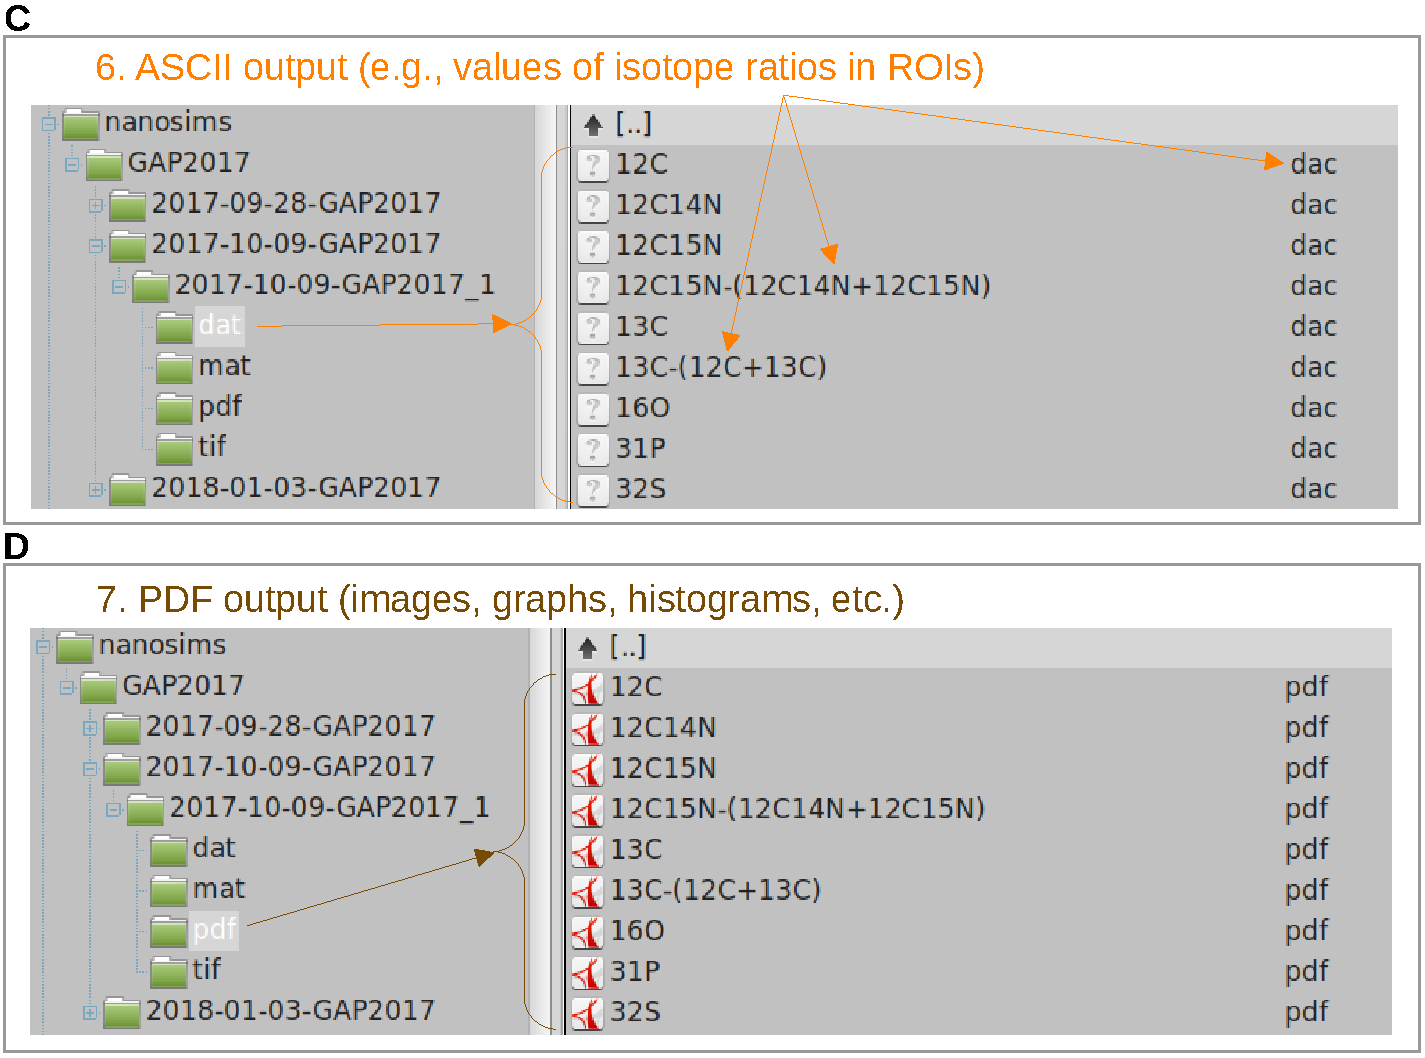
\includegraphics[width=0.485\textwidth,valign=t]{figs2/folders_organizationCD}
\end{tabular}
\caption{\label{fig2:data_organization}%
	Visualization of the hierarchical organization of raw and processed nanoSIMS data implemented in Look@NanoSIMS. %
  \textbf{(A)} The root folder (\ttt{nanosims}) contains a~project-specific sub-folder (e.g., \ttt{GAP2017}), which contains sub-folders with data measured on different days (e.g., \ttt{2017-09-28-GAP2017}, \ttt{2017-10-09-GAP2017}). %
  The `day folder' contains \emph{multiple raw datasets} measured on that particular day (\ttt{im} or \ttt{im.zip} files). %
  When a particular raw dataset is processed and analyzed, the data is stored in a `dataset folder' with the \emph{same name} as the dataset (see red ``!''). %
  \textbf{(B)} The `dataset folder' contains files defining the processing steps, including alignment information (\ttt{xyalign}), definition and classification of regions of interest (\ttt{cells.mat} and \ttt{cells.dat}, respectively), preferences (\ttt{prefs.mat}), and a comprehensive summary of results exported in a PDF file (\ttt{OutputG.pdf}). %
  The `dataset folder' also contains sub-folders with output generated by LANS in different formats. %
    \textbf{(C)} The ROI-specific ion counts and ion count ratios (\ttt{dac} files) are stored in the \ttt{dat} folder. %
    \textbf{(D)} The images, graphs, histograms, etc., are stored in the \ttt{pdf} folder.}%
\end{figure}

%\section{A typical data processing session with LANS --- an overview}

\purplebox{}
This section provides a \emph{quick summary} of steps taken during a typical data processing session with LANS. Refer to Sections~\ref{sec:level1} and \ref{sec:level2} for more details, depending on the level of analysis. 
\tcbe

%%

\subsection{Analysis of a single dataset --- starting from ``scratch''}
\label{sec:analysis_from_scratch}
\setcounter{step}{0}

\goldbox{}
The following steps will bring you from a raw dataset to basic output such as images or ROI-specific values of ion counts and ion count ratios. More details are provided in Section~\ref{sec:level1}.
\tcbe

\s{Select \lans{Input} $\ra$ \lans{dead-time and QSA correction settings} to enable dead-time and QSA (quasi-simultaneous arrival) corrections.}

\s{Select \lans{Input} $\ra$ \lans{Load RAW dataset} to load raw data from disk. The raw data is stored in an \ttt{im.zip} or \ttt{im} file depending on whether it has been compressed or not.}

\s{Select \lans{Input} $\ra$ \lans{Autoscale plane images} to automatically set the scale for all masses. }

\s{Select \lans{Input} $\ra$ \lans{Display plane images for all masses} to view the raw data as images, one plane at a time, displayed with a scale specified in the previous step. }

\s{Define \lanstf{base mass for alignment} and then select \lans{Input} $\ra$ \lans{Display alignment mass} to check the data plane by plane, \lanscb{deselect planes} with artifacts or corrupt data, and \lans{define a region} for performing a drift-correction. }

\s{Select \lans{Input} $\ra$ \lans{Accumulate plane images} to accumulate drift-corrected ion counts over selected planes. }

\s{Select \lans{Input} $\ra$ \lans{Autoscale accumulated images} and then \lans{Input} $\ra$ \lans{Display accumulated images} \lans{for all masses} to display the accumulated ion count images for all masses and export them in a PNG file.}

\s{Define \lanstf{expressions} for ion count ratios and the corresponding \lanstf{scales}. }

\s{If you want to quantify ion counts and ion count ratios in regions of interest (ROIs), select \lans{ROIs} $\ra$ \lans{INTERACTIVE ROIs definition tool} to define the ROIs and store them on disk. Additionally, you can clasify the ROIs via \lans{ROIs} $\ra$ \lans{Classify} $\ra$ \lans{manually} or \lans{automatically}.}

\s{Select \lans{Output} $\ra$ \lans{Display masses} or \lans{Output} $\ra$ \lans{Display ratios} to perform various types of data analysis and visualization, including:

\begin{itemize}
\item[--] display \lanscb{images}, \lanscb{depth profiles in ROIs}, \lanscb{lateral profiles}, or \lanscb{histograms},
\item[--] \lanscb{combine images as RGB} overlays,
\item[--] \lanscb{plot x-y-z graphs} (scatter plots) of ROI-specific ion counts or ratios,  
\item[--] \lanscb{compare ROIs} with respect to ion counts or ratios using simple statistical methods.
\end{itemize}
%
}

\nb{Note that the appearance of the output can be tweaked via \lans{Preferences} $\ra$ \lans{Additional output options}, as described in more detail in Section~\ref{sec:appearance}.}

\s{Select \lans{Output} $\ra$ \lans{Generate LaTeX + PDF output} to export results of your analysis in a~comprehensive PDF file.}

\s{Select \lans{Preferences} $\ra$ \lans{Store preferences} to save the settings of the current data processing session in a file (we recommend to use the file name \ttt{prefs.mat}). This is useful when you want to return to the analysis of the same file in the future, and essential if you want to later on merge all the results of your analyses of multiple datasets (``metafile processing''), as explained below. Therefore, it is highly recommended that you do this.}

\s{Optionally, select \lans{Preferences} $\ra$ \lans{Create full backup of processed data} to back up the processed data in a compressed (\ttt{zip}) file. This is useful for sharing the results of your data processing and analysis with collaborators.}

%%

\subsection{Continuation of a previously stored single-dataset analysis}
\setcounter{step}{0}

\goldbox{}
If you want to continue with the analysis of a dataset that you have analysed previously, you can save some time by following these steps:
\tcbe

\s{Select \lans{Input} $\ra$ \lans{dead-time and QSA correction settings} to enable dead-time and QSA (quasi-simultaneous arrival) corrections.}

\s{Select \lans{Input} $\ra$ \lans{Load+accumulate+display RAW or PROCESSED dataset}. After you select the raw data and preferences files (\ttt{im.zip} or \ttt{im} file and \ttt{prefs.mat}, respectively), the data will be loaded, drift-corrected, accumulated and displayed automatically.}

%\addon{You will be prompted to select the raw data (\ttt{im.zip} or \ttt{im} file) as well as the preferences file (e.g., \ttt{prefs.mat}). }

%\addon{After you do that, steps 2 (loading), 6 (drift-correction and accumulation) and 7 (display) described in Section \ref{sec:analysis_from_scratch} will be performed automatically.}
 
\s{Select \lans{ROIs} $\ra$ \lans{Load ROIs from disk} to load the previously defined ROIs from disk.}

%\addon{Choose the previously selected ROIs file, e.g., \ttt{cells.mat}. Modify ROIs definition or classification, if required.}

%\item Continue with steps 13--15 described in Section~\ref{sec:analysis_from_scratch}.

\nbx{After completing these steps, you can continue with further processing and analysis as described in the previous section (steps 8--13).}

%%

\subsection{Analysis of multiple datasets --- ``metafile processing''}
\setcounter{step}{0}

\goldbox{}
After the analysis of several single datasets, you are left with isotope ratio values and images scattered across \bb{multiple} files and folders. You can quickly \bb{merge} these multiple files into \bb{one} output file using the following steps. More details are provided in Section~\ref{sec:level2}.
\tcbe

\s{Ensure that the raw and processed data are organized as described in Section~\ref{sec:data_organization} (see Fig.~\ref{fig2:data_organization}).}

\s{Select \lans{Process multiple} $\ra$ \lans{Generate metafile} to define a list of datasets that will be analyzed together.}

%\addon{Typically, the datasets selected in the list are part of a~project or correspond to a~particular set of treatments within a~project.}

\s{Select \lans{Process multiple} $\ra$ \lans{Process metafile} to perform the analysis of multiple datasets.}

%
\nbx{The output generated by metafile processing can be used for visualization and further analysis (e.g., statistical analysis) by LANS or other, third-party software.}

%\section{Less common data processing in LANS --- an overview}

\purplebox{}
Over the years, different ways of analysis and visualization of nanoSIMS data have been added to LANS. Although they may be useful only under special circumstances, it is good to know about them, just in case. 
\tcbe

\noindent
The most noteworthy ones include:

\begin{enumerate}

\item \lanscb{Hue intensity modulation} of ratio images based on rescaled ion counts.

\item Integrating an \lans{external image} into the nanoSIMS dataset. This includes \lans{alignment} and \lans{overlays} of external and nanoSIMS images, definition of \lanstf{ROIs based on the external image}, and \lans{resampling} of nanoSIMS data to match the resolution of the external image.

\item Loading datasets in \lans{blocs}, including the possibility to load and combine \emph{multiple} raw datasets (measured using a~chain analysis of the same sample area) and analyze them as one dataset.

\item Visualization of \lanscb{lateral profiles across depth}.

\item Loading datasets with more than 8 masses. Such datasets can be acquired using the peak-switching mode, and they can contain up to 16 masses.

%\item Automatic ROI classification.

\end{enumerate}
%
More details about these analyses are provided in Section~\ref{sec:level3}.

%\section{Tweaking the appearance and type of LANS output}
\label{sec:appearance}

\purplebox{}
Before you do any serious work with LANS, it is good to know that the appearance of the graphical output generated by LANS may \bb{not} be the same if produced by different versions of Matlab or if you work with LANS under Windows, Linux or MacOS. This section describes how to resolve this issue. Note that you will need to deal with this issue only once, at the very beginning of working with LANS, as the system-specific settings will be stored on your computer (in a~file called \ttt{nanosimsini.mat} in your home folder) when you close LANS and then reloaded when you start it the next time. 
\tcbe

\subsection{Adjusting the font size in the generated images and graphs}
\setcounter{step}{0}

\goldbox{}
The most prominent examples of where the differences occur include the appearance of the title and axis labels. Depending on the system and Matlab version, they can appear too large or too small relative to the size of the graph or image. Use the following steps to make the adjustments that suit your needs. 
\tcbe

\s{Select \lans{Preferences} $\ra$ \lans{Additional output options}.}

\s{In the new window that opens (Fig.~\ref{fig:appearance}), you will find several parameters in the  \lanstf{Magnification} \lanstf{printing factors} box. Adjust these factors individually for a~specific type of output, such as ion and ratio images, scatter plots, etc., and click \lans{Apply}.}

\sbx{Export an image or a graph (see below to learn how to do this) and check how it looks like.}

\s{You can also modify the font size by changing the value in the \lanstf{Fontsize of \dots} field.}

\nb{It is recommended that you experiment with the magnification factors a~little to get optimal results for your needs and taste.}

\nnb{If you reexport an image but the results do not seem to reflect the newly applied settings, you will need to close the image and export it again. This is because some features are only updated if the image is displayed anew.}

\begin{figure}[!t]
\centering
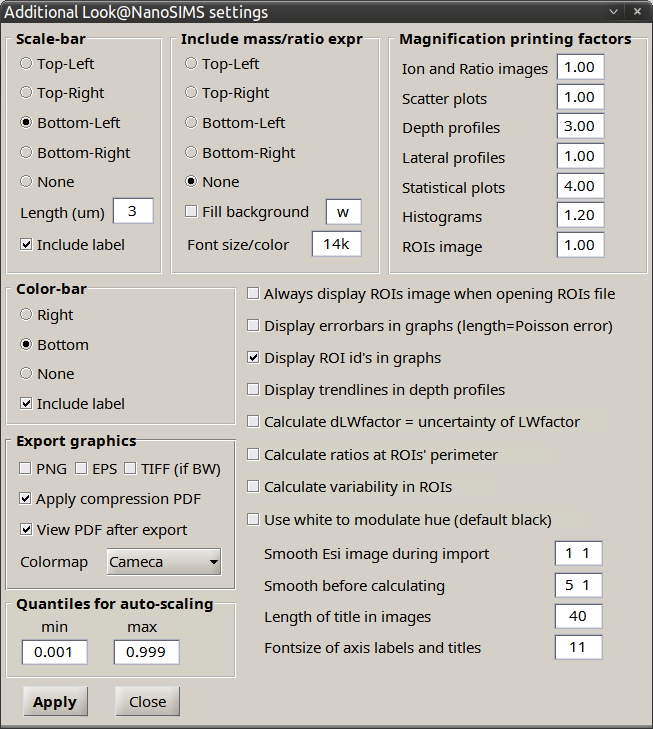
\includegraphics[scale=0.5]{figs1/LANS-tweaking}
\caption{\label{fig:appearance}%
Additional output options that can be tweaked in LANS.}
\end{figure}

\subsection{Further adjustments}
\label{sec:appearance1}

\goldbox{}
The \lans{Additional LANS settings} window (Fig.~\ref{fig:appearance}) offers multiple other options for tweaking the appearance or type of output generated by LANS. Their thorough explanation goes beyond the scope of this document. Instead, you are encouraged to experiment and explore them by yourself. Here, we only highlight the ones that are most commonly used. Examples of the possible results are shown in Fig.~\ref{fig:appearance2}.
\tcbe

\nnb{\lanscb{\bb{Color bar}}: Color bar is relevant when displaying images of ion counts or ion count ratios. It can be placed below or to the right from the image. Relevant for this setting is the actual \lans{Colormap} (i.e., the correspondence between the value and color) in which the image is displayed. LANS offers numerous colormaps, which can be selected in the \lans{Export graphics} box.}

\nnb{\lanscb{\bb{Scale bar}}: Including a~scale bar is important when exporting images. You can specify its location within the image (top or bottom, left or right) and length (in $\mu$m). You can also specify whether the label of the scale bar, or the scale bar itself, should be included or not.}

\nnb{\bb{Title and annotation:} When working with mutliple datasets, it is useful if the generated output contains information that identifies the dataset and the variable displayed. In LANS, this information is included in the title and annotation of the graph or image. Whether or not the title should be included can be specified by checking the \lanscb{Graphs/image title} checkbox in the main LANS window, whereas settings in the \lanscb{Include mass/ratio expr} box in the \lans{Additional LANS settings} window can be used to specify how to include additional annotatation.}

\nnb{\bb{Auto-scaling}: You can automatically set the scale of a~particular image by entering \ttt{[auto]} in the corresponding \lanstf{scale} field. The minimum and maximum of the scale is calculated, respectively, based on the \lanstf{min} and \lanstf{max} quantiles specified in the \lanscb{Quantiles for auto-scaling} box. }

\nnb{\bb{ROI annotation}: When displaying scatter plots, you can \lanscb{add ROI identification numbers} to each displayed data-point or \lanscb{include error-bars} indicating measurement precision (quantified by the Poisson error) by checking the corresponding checkboxes in the \lans{Additional LANS settings} window.}

%%

\begin{figure}[!ht]
\centering
\begin{tabular}{ccc}
A: 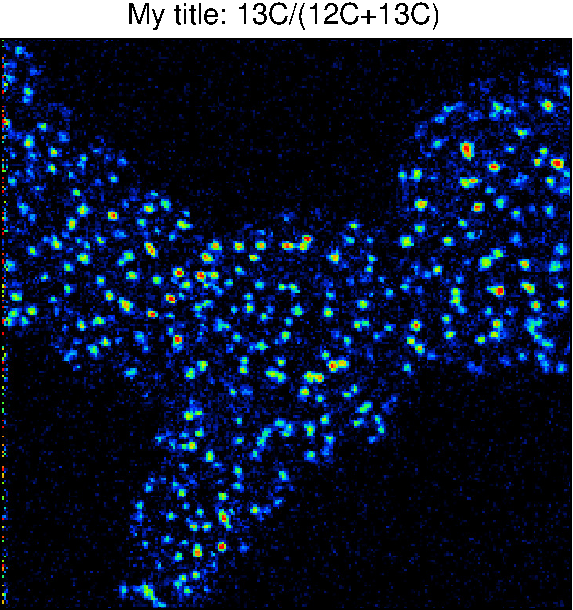
\includegraphics[scale=0.4, valign=t]{figs4/a-13C-(12C+13C)}
& 
B: 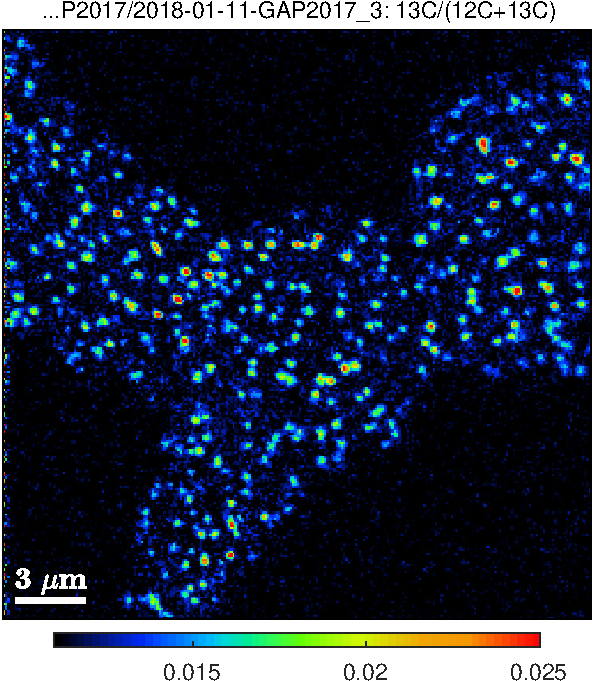
\includegraphics[scale=0.4, valign=t]{figs4/b-13C-(12C+13C)}
&
C: 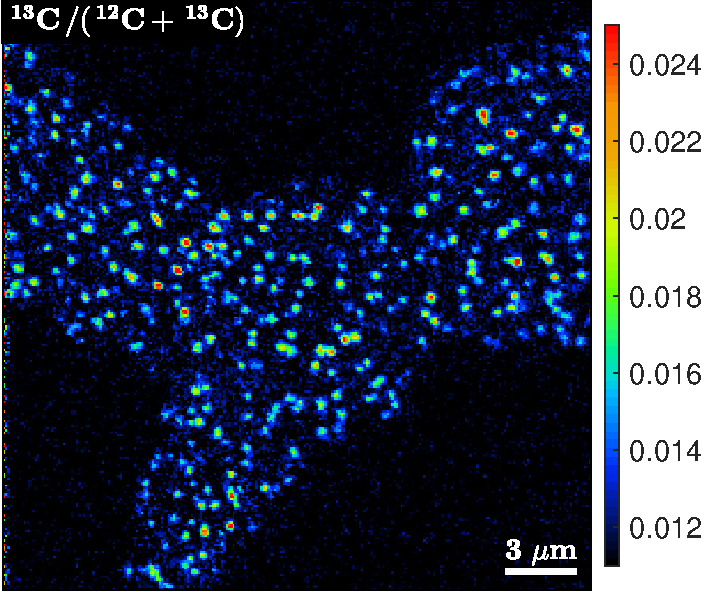
\includegraphics[scale=0.4, valign=t]{figs4/c-13C-(12C+13C)}
\end{tabular}
\\[5mm]
\begin{tabular}{ccc}
D: 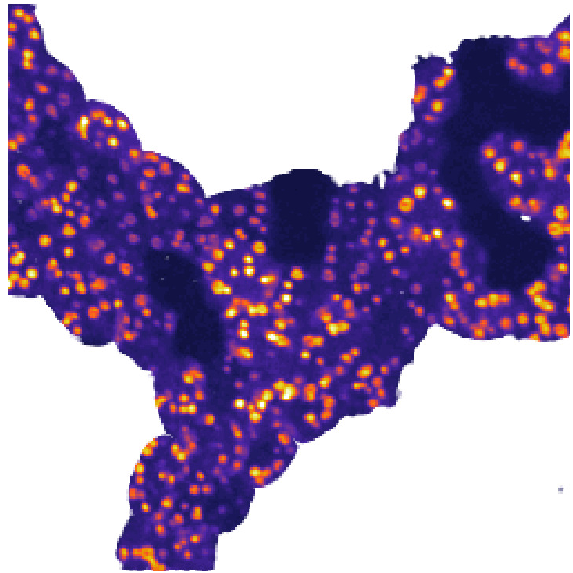
\includegraphics[scale=0.4, valign=t]{figs4/a-15N-14N}
& 
E: 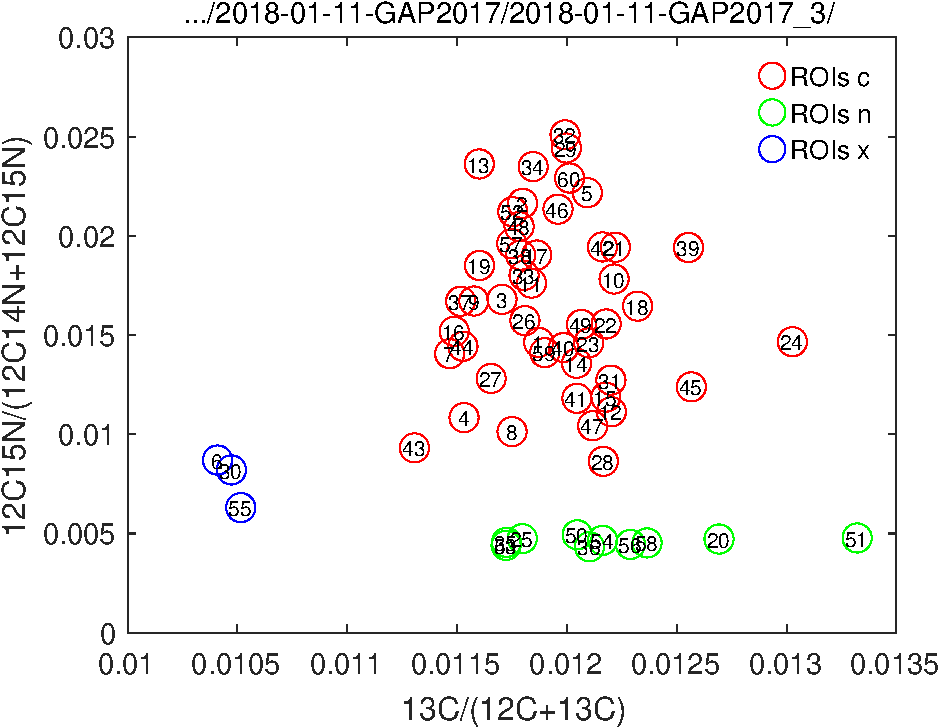
\includegraphics[scale=0.28, valign=t]{figs4/a-13C-15N}
&
F: 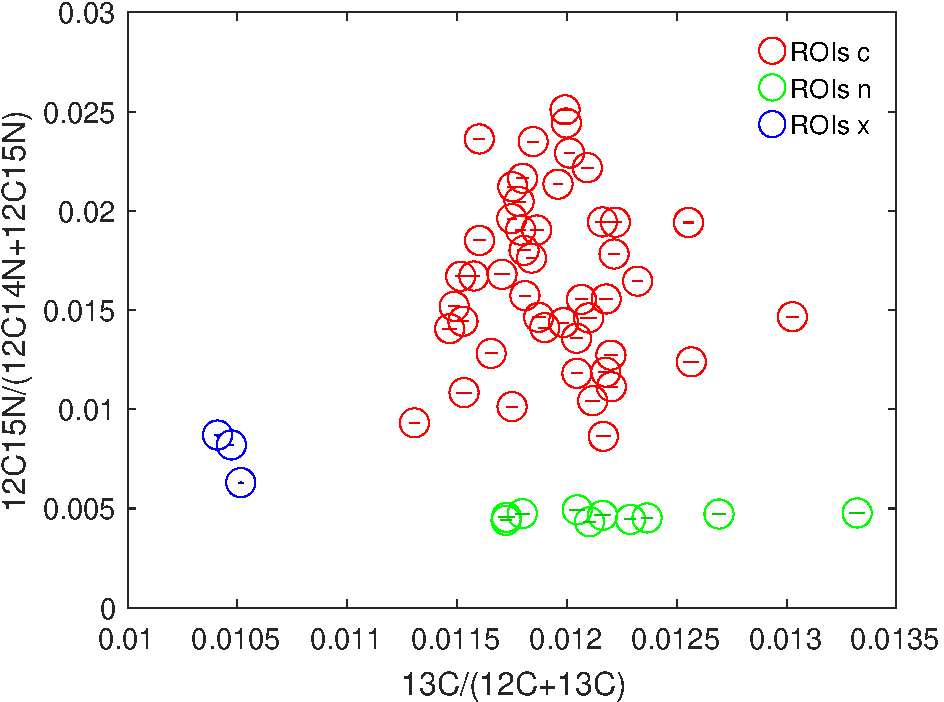
\includegraphics[scale=0.28, valign=t]{figs4/b-13C-15N}
\end{tabular}
\caption{\label{fig:appearance2}%
Examples of images and graphs generated by LANS. Panels A--C show different types of information and annotation that can be included in the images, including the title, color bar, scale bar, or formula of the displayed quantity. Panel D shows an image displayed in a~different colormap, without any annotation. Panels E and F show scatter plots with ROI identifiers and error-bars included, respectively.}
\end{figure}

%\section{Analysis of a single dataset --- starting from ``scratch''}
\label{sec:level1}

This section describes in greater detail how to get from a raw dataset to basic output such as images or ROI-specific values of ion counts and ion count ratios. As an example, we will use the dataset \ttt{2018-01-11-GAP2017\_3.im.zip}. This dataset is available in the same location as the source files of the Look@NanoSIMS program.

At the very beginning, it is useful to note that when working with LANS, you will likely create many graphs and images, each displayed in a~separate window, which may clutter your screen. Select \lans{Output} $\ra$ \lans{Close all figures} in the main LANS window, or press~\ttt{Ctrl+g}, any time during the processing session, to quickly close all figures at once.

%\addtolength{\parskip}{2mm}

\subsection{Load nanoSIMS dataset from disk}
\setcounter{step}{0}

\s Select \lans{Input} $\ra$ \lans{Dead-time and QSA correction settings} to enable dead-time and quasi-simul\-ta\-neous arrival (QSA) corrections. Define the relevant parameters in the window that opens (Fig.~\ref{fig:dtqsa}). The corrections will be applied based on these parameters \bb{during loading} of the raw data. Note that you can specify the parameters for up to 16 masses. This can be relevant if the dataset was acquired using a peak-switching mode. If you do not know what the correct parameters are, it is better if you do not apply these corrections.

\begin{figure}[!h]
\centering
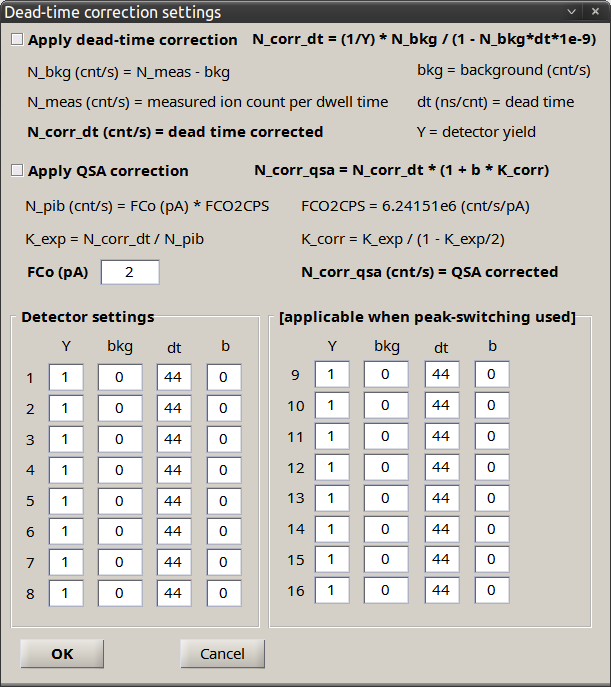
\includegraphics[scale=0.4]{figs1/LANS-dt-qsa-settings}
\caption{\label{fig:dtqsa}%
LANS window where you can adjust settings for dead-time and QSA corrections.}
\end{figure}

\s Select \lans{Input} $\ra$ \lans{Ask for range of planes and masses before loading} if you want to interactively define \bb{a range of} planes and masses that should be extracted during loading of the raw dataset. This is unnecessary in most cases, but it may be useful if your dataset is huge (e.g., more than 1~GB of data) and the memory (RAM) on your computer is insufficient.

\s Select \lans{Input} $\ra$ \lans{Shift columns or rows when loading raw data}. This data correction is relevant for data acquired by the NanoSIMS 50L instrument at Utrecht University and probably very few others around the world. It concerns a glitch in the acquisition software, which causes the data in pixels from the first column (or row) to appear in the last column (or row), or vice versa. This option allows you to \bb{shift} the pixels to the \bb{correct} position during loading of the raw dataset by entering 1 and 0 in the corresponding fields (Fig.~\ref{fig:shiftrowcolumn}). You can skip this step if this is not an issue in your dataset.

\begin{figure}[!ht]
\centering
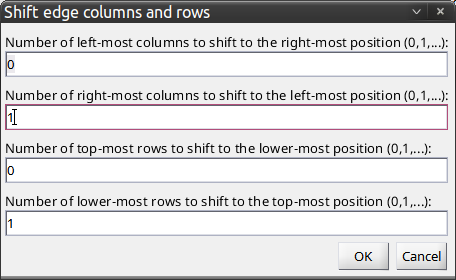
\includegraphics[scale=0.5]{figs1/LANS-shift-rows-columns}
\caption{\label{fig:shiftrowcolumn}%
LANS window where you can adjust how rows and columns in the input raw image data should be shifted during loading.}
\end{figure}

\s Select \lans{Input} $\ra$ \lans{Load RAW dataset} to load the raw dataset from disk in a standard way (i.e., plane by plane). When searching for the dataset, choose the file type: \ttt{im.zip} or \ttt{im}, depending on whether the raw data has been compressed or not. After selecting the raw data file, observe the progress of loading in the Matlab console. 

\bul When the loading is finished, names of the masses will automatically be filled in the corresponding \lanstf{mass} text fields. Additionally, \ttt{[]} will be added in the \lanstf{planes} text field, which stands for ``all planes''.

\bul Sometimes, the mass name entry in the binary \ttt{im} file is incorrectly saved. If this happens, a~``strange-looking'' name such as \ttt{au32} will be filled as the corresponding \lanstf{mass}, referring to the actual mass detected (in atomic units). If you know that the detected isotope was (in this example) ${}^{32}$S, you can rewrite the string from \ttt{au32} to \ttt{32S} and use it as the name of the mass in further analysis.

%%

\subsection{Display of mass images plane-by-plane}
\setcounter{step}{0}
\label{sec:display-masses-plane-by-plane}

\s Select \lans{Input} $\ra$ \lans{Autoscale plane images} to automatically fill in the \lanstf{scale} for each detected mass. The scale, in the form of \ttt{[min max]}, is calculated as the 0.001 and 0.999 quantile of the ion counts across all pixels and planes. The quantiles can be adjusted using \lans{Preferences} $\ra$ \lans{Additional output options} (see auto-scaling in Section~\ref{sec:appearance1}). 

\s In the \ttt{Detected masses} box, check the \lanscb{checkboxes}  to the left from the \lanstf{masses} to select which masses will be displayed in the following step. By default, all masses are selected, but you may want to change it.

\s Select \lans{Input} $\ra$ \lans{Display plane images for all masses} to view secondary ion counts detected in individual planes for all masses (Fig.~\ref{fig:displayplanes}). This is the actual data in its \bb{rawest} form, i.e., ion counts per pixel per plane.

\begin{figure}[!ht]
\centering
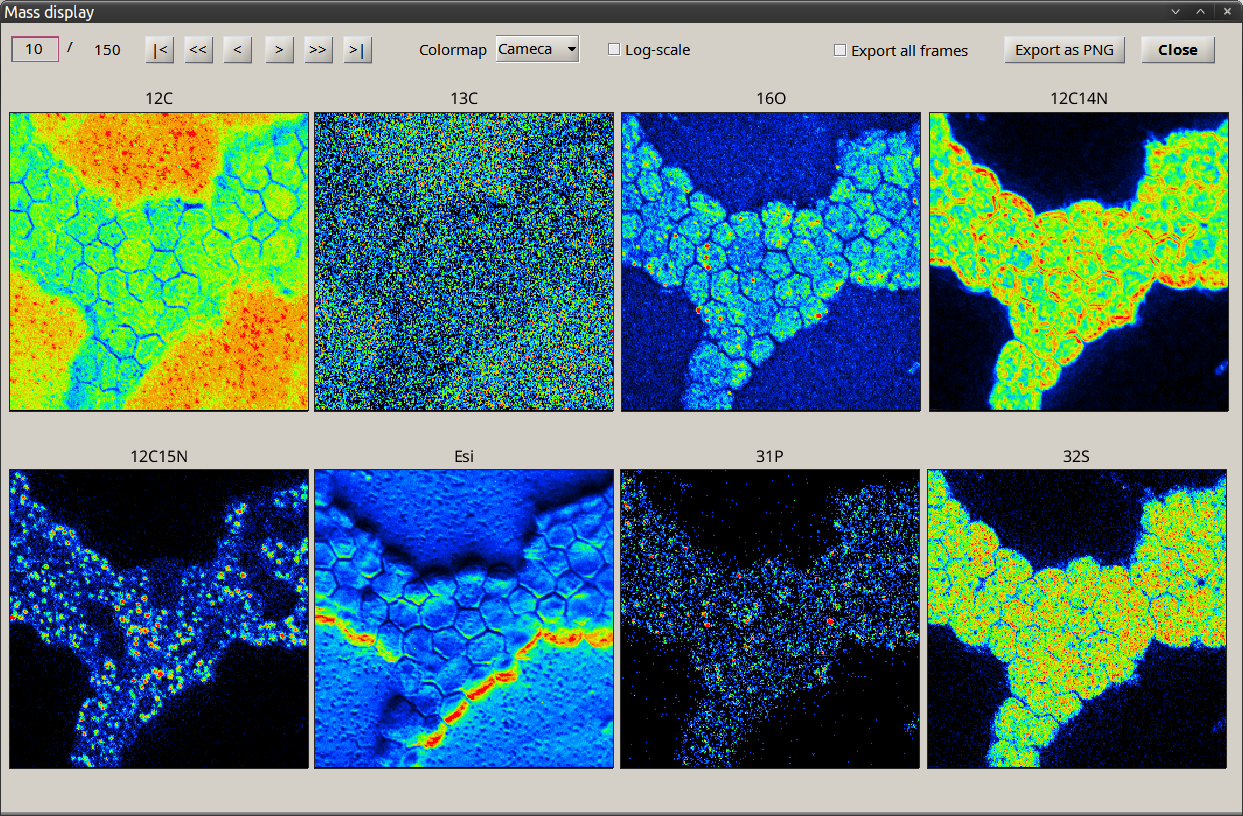
\includegraphics[width=\textwidth]{figs3/LANS-display-planes-raw}
\caption{\label{fig:displayplanes}%
LANS window for viewing the raw image data for all detected masses, plane by plane.}
\end{figure}

\bul Use arrows to browse through the planes forward and backward.

\bul Click on \lans{Export as PNG} to export all masses in a particular plane as a PNG file. If you additionally check \lanscb{Export all}, you can export all planes, each into a separate PNG file.

\bul
When browsing through the ion count images, you can often notice a small \bb{drift} when going from one plane to the next. This drift is caused by temperature instabilities during the measurements (a~bigger jump can also be caused by an~earthquake!). You will be able to correct for this drift in the next step. At this point, you should decide on the mass that will be used to calculate the drift correction (called \lanstf{Base mass for alignment}). As a~rule of thumb, it should be one with a relatively \bb{high ion counts} and \bb{clear contrast} across the image. In this example, it will be \ttt{12C14N}.

%%

\subsection{Drift-correction and accumulation of planes}
\setcounter{step}{0}
\label{sec:drift-correction-accumulation}

The drift-corrected accumulation of planes is controlled by settings specified in the \ttt{Accumulation options} box and by the numbers in the \lanstf{planes} list (Fig.~\ref{fig:alignoptions}). 

\begin{figure}[!ht]
\centering
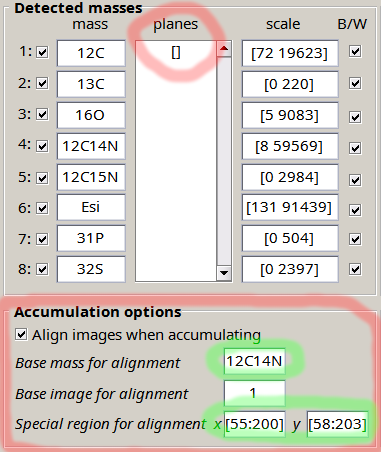
\includegraphics[scale=0.4]{figs3/LANS-main-alignment}
\caption{\label{fig:alignoptions}%
Parts of the main LANS window relevant for controling drift-correction of planes.}
\end{figure}

\s Specify the \lanstf{Base mass for alignment}. This is done based on your choice made in the previous step (in this example: \ttt{12C14N}). 

\s Select \lans{Input} $\ra$ \lans{Display alignment mass}. 

\bul In the new window that opens (Fig.~\ref{fig:show-alignment-mass}), click on \lans{arrows} to browse through the individual planes. 

\begin{figure}[!ht]
\centering
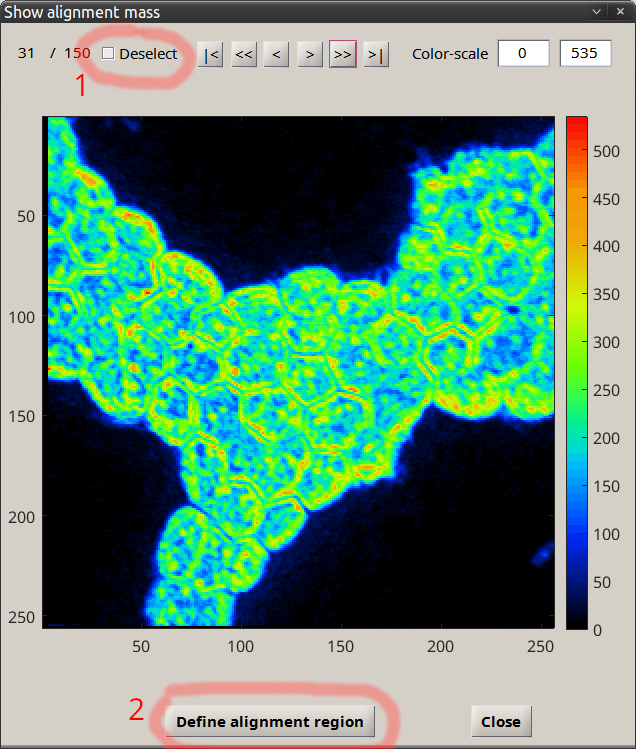
\includegraphics[scale=0.4]{figs3/LANS-show-alignment-mass}
\caption{\label{fig:show-alignment-mass}%
LANS window where you can (1) specify planes that should be excluded during accumulation and (2) define a~region based on which drift-correction will be calculated.}
\end{figure}

\bul Check \lanscb{Deselect} to mark the plane that should be excluded from accumulation (e.g., if the data in that plane is corrupt).

\bul After you have completed the plane selection, click on the \lans{Define alignment region} button to define an area in the image based on which the drift correction will be calculated in the next step. It is recommended to define this area as a~minimum rectangular region in the image that contains pronounced spatial heterogeneities (such as a cell or a group of cells). Close the window when you have defined the area.

\bul After you close the window, the x and y ranges of the alignment region will be written in the respective fields of \lanstf{Special region for alignment} (Fig.~\ref{fig:alignoptions}). Also, the range of selected planes will be written in the \lanstf{planes} list. You can edit these fields if you know the correct values, but be careful not to make any syntax errors. 

\s Check \lanscb{Align images when accumulating} if you want to apply automated drift correction during the accumulation of planes. If not, which is rarely the case, leave this checkbox unchecked.

\s Back in the main LANS window, select \lans{Input} $\ra$ \lans{Accumulate plane images} to start the accumulation of drift-corrected images. 

\bul You will be asked whether to employ a \lans{New} or \lans{Old} algorithm. In most cases, you will choose the new one. However, the old one is preferred if the drift-correction is based on images with very low ion counts (i.e., very pixelated images).

\bul Observe the drift-correction progress in the Matlab console. 

\bul When the drift-correction information is calculated for all selected planes, you will be prompted to accept or reject it (Fig.~\ref{fig:drift-correction}). 

\begin{figure}[!ht]
\centering
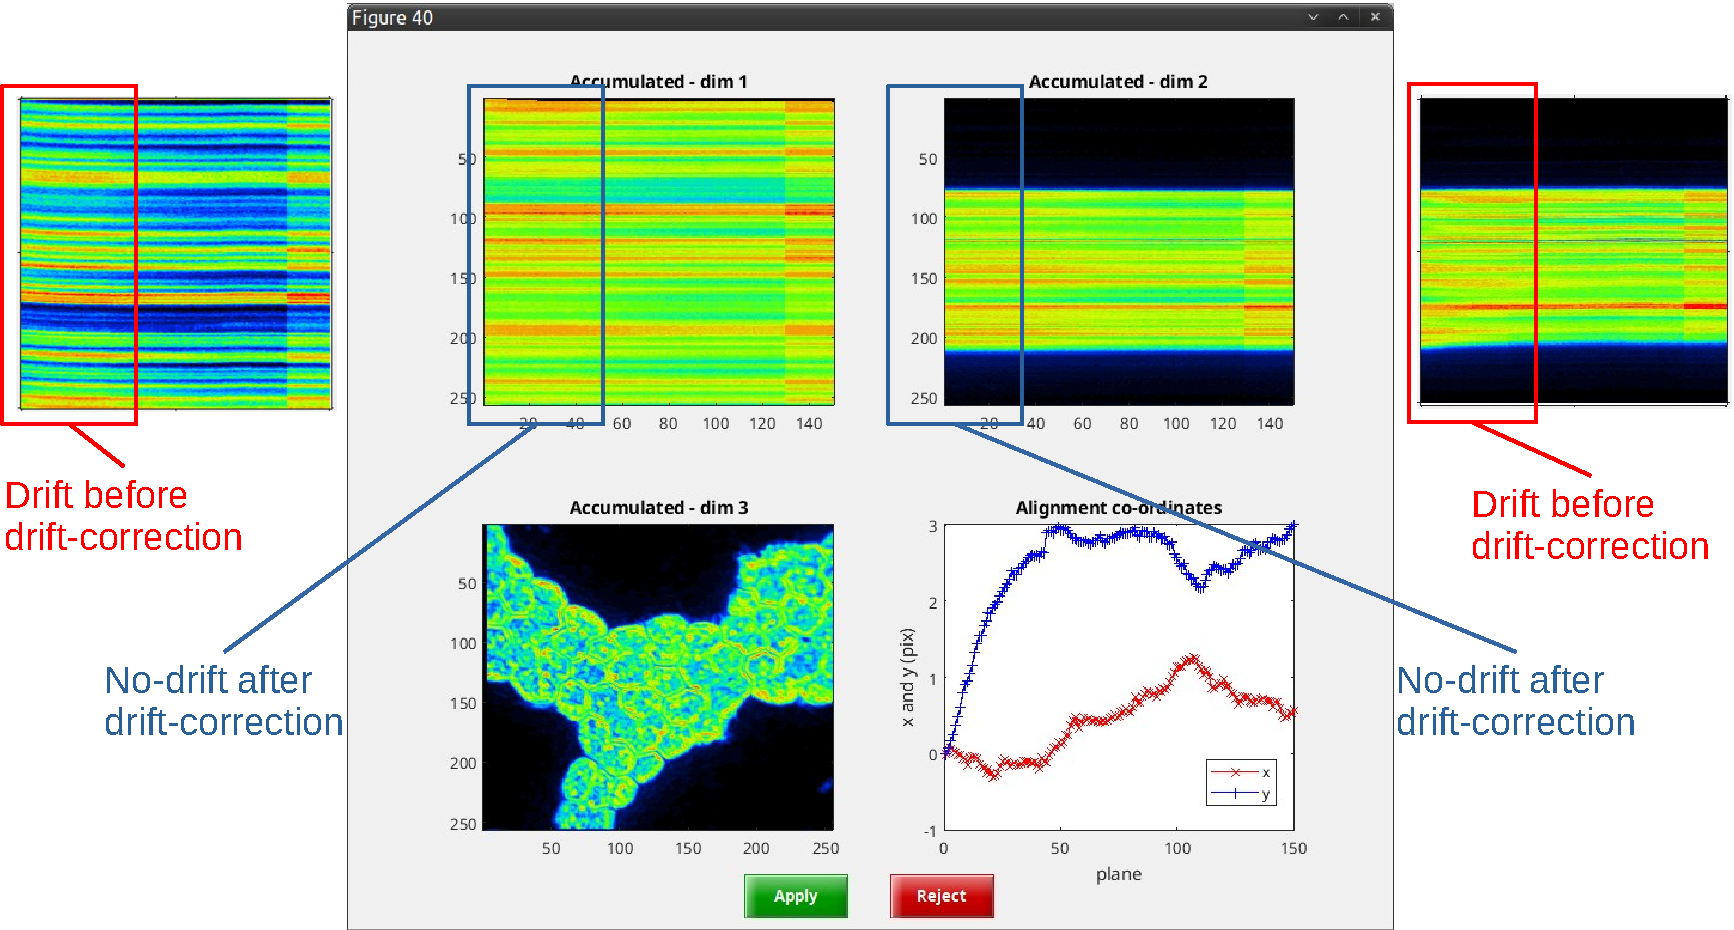
\includegraphics[width=\textwidth]{figs3/LANS-drift-correction}
\caption{\label{fig:drift-correction}%
LANS window showing the results after calculating the drift-correction (central window). For comparison, the original ion count data along a~vertical and horizontal profile through the center of the image are also shown (to the left and right of the central window). In this example, the drift along the vertical ($y$) direction was pronounced during the initial 50 planes (by about 3~pixels), then decreased. The drift in the horizontal ($x$) direction did not exceeed about 1.5 pixels across the 150 planes. The drift-correction is considered good if the two images in the top row (`Accumulated dim 1 and 2') show \bb{flat horizontal stripes}, in contrast to `wiggly' stripes visible in the data before drift correction.}
\end{figure}

\bul If you \lans{accept} it, the information will be stored in the file \ttt{xyalign.mat} and all planes for all masses will be accumulated based on this information. Also, this information will automatically be used in the future if you load the raw dataset using \lans{Input} $\ra$ \lans{Load+accumulate+display RAW or PROCESSED dataset}.

\bul If you \lans{reject} it, you can reiterate the previous steps (1--4) until you arrive at a dataset with drift-corrected and accumulated planes.

\bul Note that you do need to accumulate the planes, because most of the subsequent data processing steps only work for the ion counts accumulated over all (selected) planes.

\bul If you realize, anytime at a later point during your data processing, that you are not satisfied with the drift-correction, you need to first delete the \ttt{xyalign.mat} file (via \lans{Preferences} $\ra$ \lans{Remove xyalign.mat from disk}), then \lans{Load RAW dataset}, and then repeat the previous steps (1--4) to drift-correct and accumulate the planes again.

%%

\subsection{Display accumulated mass images}
\setcounter{step}{0}

\s Back in the main LANS window, select \lans{Input} $\ra$ \lans{Autoscale accumulated images} to update the \lanstf{scale} fields with a range optimized for displaying accumulated mass images. 

\bul The optimum scale is calculated as the 0.001 and 0.999 quantiles of the accumulated ion counts across the image pixels. These quantiles can be adjusted via \lans{Preferences} $\ra$ \lans{Additional output options}.

\s Alternatively, define the \lanstf{scale} \bb{manually} by typing in the \ttt{[min max]} (minumum and maximum) values by yourself. If you then press \ttt{Enter}, the corresponding mass will be displayed in a new window using the color scale defined by the specified range. You can repeat this many times to \bb{quickly adjust} the color scale for optimal display (e.g., to achieve best contrast).

\bul Note that you can display the images in multiple colormaps. These can be adjusted via \lans{Preferences} $\ra$ \lans{Additional output options} (see Section~\ref{sec:appearance1}). Explore them to find the best you like. If you want to display the images in grayscale, click on the corresponding \lanscb{B/W} checkbox next to the scale.

\bul If there is a large contrast in ion counts across the image (e.g., by 2--3 orders of magnitude), it is often useful to display the log-transformed image. To do this, check \lanscb{Log10-transform} in the \ttt{Output options} box before you press \ttt{Enter} to display the image. When displaying log-transformed images, make sure that the minimum value of the \lanstf{scale} is greater than 0. If it is 0 and you press \ttt{Enter}, the image will be displayed in a~scale where $\ttt{min} = 0.001\times\ttt{max}$, which may not be optimal.

\s Select \lans{Input} $\ra$ \lans{Display accumulated images for all masses} to display the images, lumped together for all masses, and export them in a PNG file (Fig.~\ref{fig:display-accu-planes}). This output is useful as a~quick overview of the accumulated raw data.

\begin{figure}[!ht]
\centering
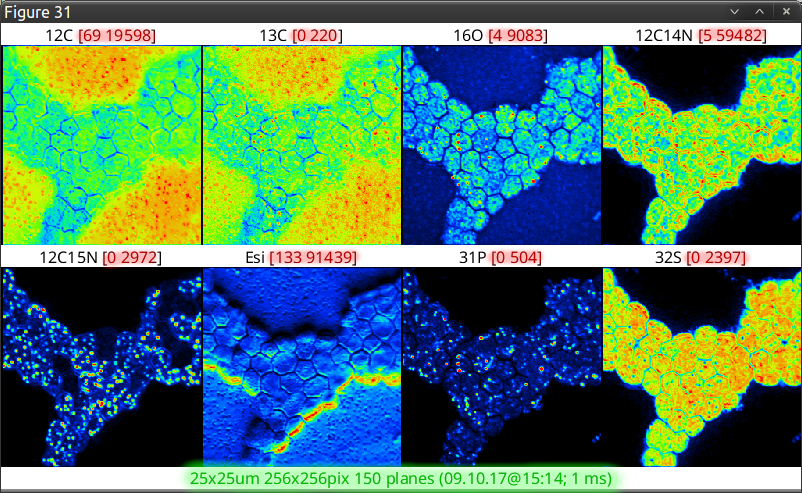
\includegraphics[width=0.9\textwidth]{figs3/LANS-display-accu-planes}
\caption{\label{fig:display-accu-planes}%
Display of ion counts after drift-correction and accumulation of selected planes. The scale is shown for each individual mass, formatted as \ttt{[min max]}. Basic information about the data, e.g., real and pixel size, date of acquisition, dwell time, is also shown (at the bottom).}
\end{figure}

\s Check \lanscb{Display images} in the \ttt{Output options} box and then select \lans{Output} $\ra$ \lans{Display masses} to display the images in a~nicer way and separately for each mass (Fig.~\ref{fig:display-masses}). 

\begin{figure}[!ht]
\centering
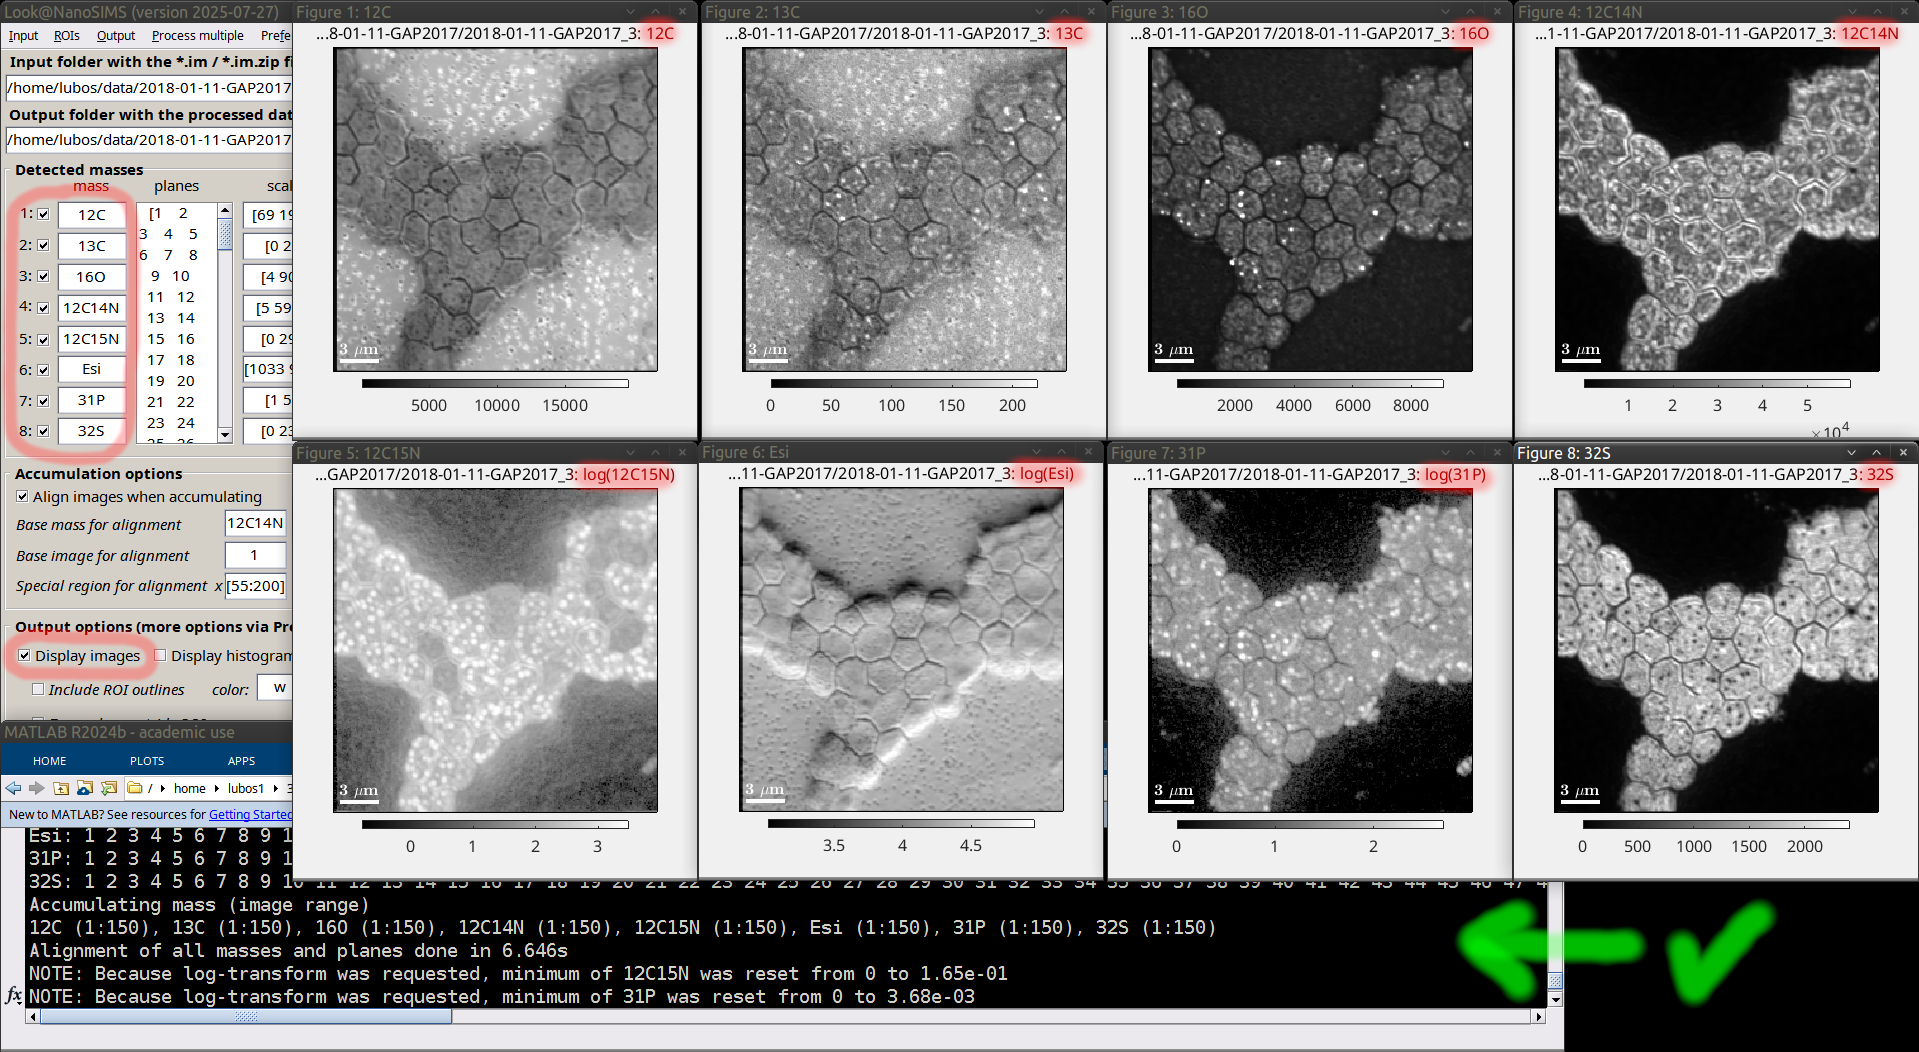
\includegraphics[width=\textwidth]{figs3/LANS-display-masses}
\caption{\label{fig:display-masses}%
Screenshot of a~LANS session showing ion count images after drift-correction and accumulation. Each mass is displayed in a~separate window, some in the linear scale, some in the logarithmic scale. Note the arrangement of the main LANS window in the top-left part of the screen and of the Matlab console at the bottom of the screen, which allows monitoring of messages reported by LANS at all times.}
\end{figure}

\bul In this step, the image appearance, including the location of the colorbar, size and location of the scale bar, etc., can be tweaked via \lans{Preferences} $\ra$ \lans{Additional output options} (see Section~\ref{sec:appearance}). 

\bul Ensure that \lanscb{Export PDF graphics} in the \ttt{Output options} box is checked to export the images as PDF (they will be stored in the \ttt{pdf} sub-folder of the current data folder).

%%

\subsection{Display ratio images}
\setcounter{step}{0}

\s Back in the main LANS window, type \bb{formulas} for calculating ratio images in the  \lanstf{expression} fields (Fig.~\ref{fig:display-ratios}). In principle, the formula can be any valid arithmetic expression containing any of the detected masses. However, it is recommended not to make the formulas too complicated. Typical examples include:

\begin{itemize}
\item \ttt{13C/12C} to calculate the $^{13}C/^{12}C$ isotope ratio,
\item \ttt{13C/(12C+13C)} to calculate the $^{13}C$ atom fraction,
\item \ttt{32S/12C} to calculate the $^{32}S/^{12}C$ ion count ratio (a proxy for the S/C elemental ratio), 
\item \ttt{31P/plane} to calculate the average $^{31}P$ ion counts per detected plane, 
\item \ttt{31P/plane/pixel} to calculate the average $^{31}P$ ion counts per plane per pixel (only applicable if ROIs are defined; see below).
\end{itemize}

\s For each expression, type in the \lanstf{scale} to the correspoding field (Fig.~\ref{fig:display-ratios}). Similar to masses, the scale should be in the form \ttt{[min max]} (minumum and maximum). 

\bul If you then press \ttt{Enter}, the corresponding ratio image will be displayed in a~new window using the color scale defined by the specified range. You can repeat this many times to \bb{quickly adjust} the color scale for optimal display.

\s Check \lanscb{Display images} in the \ttt{Output options} box and then select \lans{Output} $\ra$ \lans{Display ratios} to display the ratio images, in in a~separate window (Fig.~\ref{fig:display-ratios}). 

\begin{figure}[!ht]
\centering
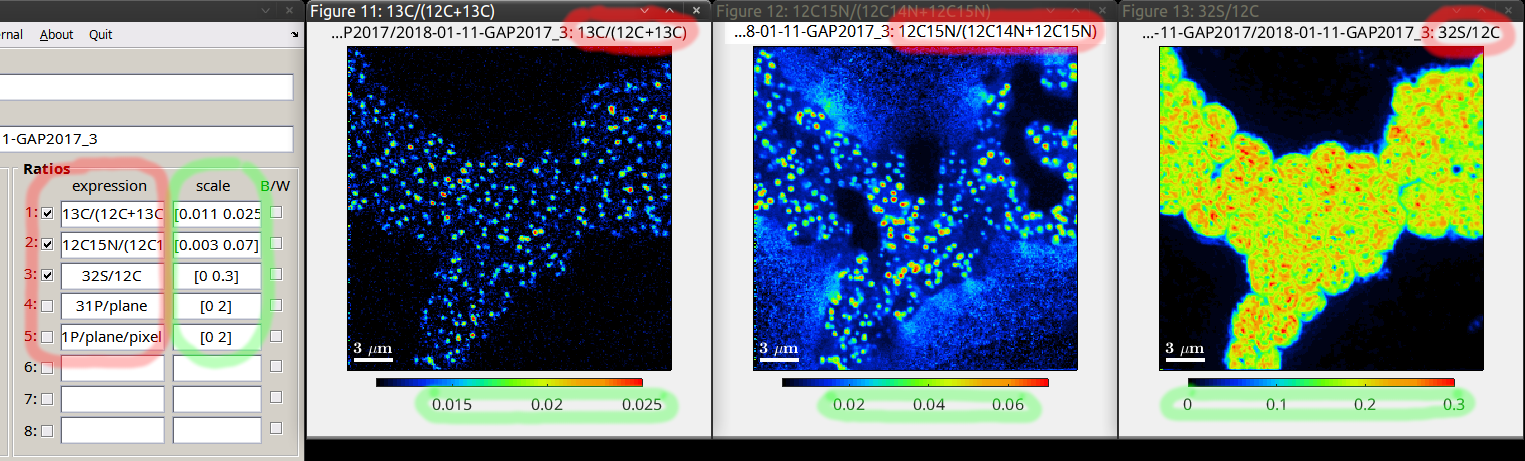
\includegraphics[width=\textwidth]{figs3/LANS-display-ratios}
\caption{\label{fig:display-ratios}%
Examples of ion count ratio images. The ratios are defined through formulas typed in the \lanstf{expression} field (marked in red), the scales are defined in the corresponding \lanstf{scale} fields (marked in green).}
\end{figure}

\bul In this step, the image appearance can be tweaked via \lans{Preferences} $\ra$ \lans{Additional output options}.

\bul Ensure that \lanscb{Export PDF graphics} in the \ttt{Output options} box is checked to export the images as PDF.

%%

\subsection{Display RGB overlays}
\setcounter{step}{0}

To increase the information value of the mass and ratio images, they can be combined and displayed as RGB overlays.

\s To specify which image will be filled in the red, green and blue channel of the RGB overlay, enter identification numbers (1--8, found to the left of the mass names or ratio expressions) in the corresponding \lanstf{R/x}, \lanstf{G/y} and \lanstf{B/z} fields (found under \ttt{Plot-x-y-z graph} in the \ttt{Output options} box) (Fig.~\ref{fig:rgb-overlay}).

\begin{figure}[!ht]
\centering
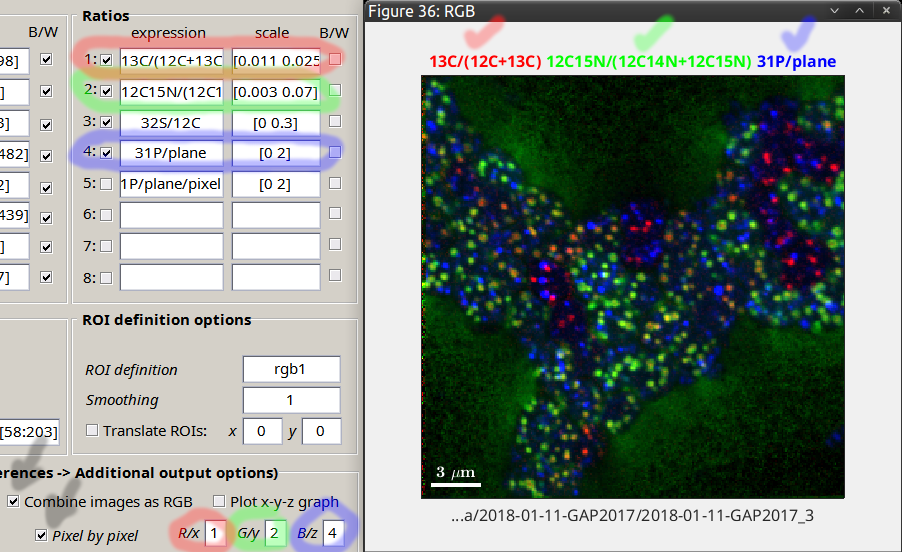
\includegraphics[scale=0.35]{figs3/LANS-rgb-overlay}
\caption{\label{fig:rgb-overlay}%
Example of an RGB overlay of ion count and ion count ratio images.}
\end{figure}

\bul At most one number per R, G and B field is allowed. If one or more of the fields is left empty, the corresponding channel(s) will be set to zero and thus appear black in the RGB overlay.

\s In the \ttt{Output options} box, check \lanscb{Combine images as RGB}. Then, check \lanscb{Pixel by pixel} to combine the images without modification and/or \lanscb{ROI-averaged} to use ROI-averaged values when creating the overlays (the latter is only possible if ROIs have been defined).

\s Select \lans{Output} $\ra$ \lans{Display masses} or \lans{Display ratios} to display the RGB overlay derived from mass or ratio images, respectively.

\bul If you want to overlay a~mass image with a~ratio image, enter the corresponding name of the mass into one of the \lanstf{expression} fields, specify the scale, enter the corresponding identification number in one of the \lanstf{color} fields (R, G or B), and then select \lans{Output} $\ra$ \lans{Display ratios} (Fig.~\ref{fig:rgb-overlay}). 

\bul You can combine multiple masses with multiple ratios by entering the corresponding identification numbers in the R, G and B fields.

\bul In addition to PDF, RGB overlay images are also exported as TIF files (in the \ttt{tif} sub-folder of the dataset folder).

%%

\subsection{Define ROIs}
\setcounter{step}{0}

Typically, much of nanoSIMS data analysis revolves around regions of interest (ROIs). There are many options for defining ROIs in LANS, as described below. Once you get used to it and learn the ``tricks'', ROI definition can be very efficient. 

We re-emphasize the importance of looking at the comments written in the Matlab console while defining ROIs. They provide more details about what to do while performing specific steps. The key constraint is: \bb{if you start an action, you \emph{must} finish it.} If you don't, the program will likely get ``stuck'' and you may need to terminate it. We won't go into details here, but briefly, this peculiarity is related to the way Matlab handles user's input in a drawing mode. Thus, beware and keep an eye on the messages in the console. You can also learn more about this topic via \lans{Help} provided in the ROI definition tool window.

\s In the main LANS window, specify the \lanstf{ROI definition template}. 

\bul This can be an individual mass, ratio, an RGB overlay of masses or ratios, or an external image.

\bul In this example, we will use an RGB overlay of \ttt{12C15N/(12C14N+12C15N)}, \ttt{12C14N} and \ttt{31P} (Fig.~\ref{fig:roi-template}). Since we want to combine ratios and masses, we enter \ttt{12C14N} as, e.g., expression~6, \ttt{31P} as expression~4, and enter the scale for both in the corresponding \lanstf{scale} field. Then, we enter \ttt{2}, \ttt{6} and \ttt{4} to the fields for \lanstf{R}, \lanstf{G} and \lanstf{B}, respectively. Finally, we enter \ttt{rgb2} as the \lanstf{ROI definition template} (entering \ttt{rgb} means that we use an RGB overlay, \ttt{2} means that we use an overlay of ratios rather than masses).

\begin{figure}[!ht]
\centering
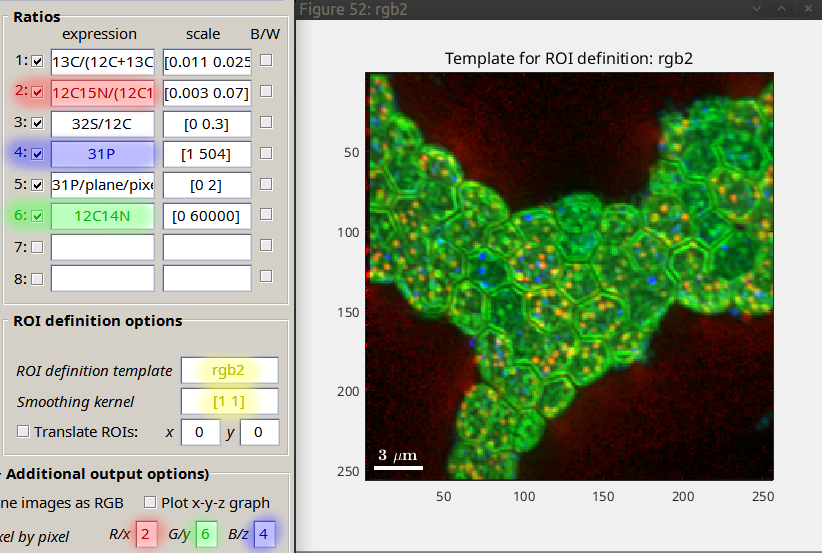
\includegraphics[scale=0.4]{figs3/LANS-roi-template}
\caption{\label{fig:roi-template}%
Example showing how to define a~ROI definition template. In this example, the template comprises an RGB overlay of three ratio images (\ttt{rgb2}).}
\end{figure}

\bul The ROI template can optionally be \bb{smoothed} before it is used for ROI definition. Smoothing is done using a median filter with a~two-dimensional kernel size (in pixels) specified in the \lanstf{Smoothing kernel} field. If applied, ROI outlines will generally be smoother if defined using the \lans{interactive thresholding} approach (see below). In this example, we will not do any smoothing and just use \ttt{[1 1]} as the smoothing kernel (Fig.~\ref{fig:roi-template}).

\s Select \lans{ROIs} $\ra$ \lans{Display template for ROI definition} to verify that the template looks as intended (Fig.~\ref{fig:roi-template}). 

\s Select \lans{ROIs} $\ra$ \lans{INTERACTIVE ROIs definition tool} to open a~window dedicated to ROI definition. 

\bul During this process, you will be prompted to select the \ttt{ROI file} (e.g., \ttt{ROIs.mat}) and \ttt{ROI classification file} (e.g., \ttt{ROIs.dat}). Select them if the files have been previously created and you want to reuse them, or press \lans{Cancel} if they do not exist (yet).

\bul If they exist and you do select them both, they will be \bb{linked}. This means that when you add or remove a~ROI from the image file, the corresponding ROI will also be added or removed from the classification file. This will be explained in more details later on.

\vskip5mm\noindent
After these steps, a new window will open (Fig.~\ref{fig:roi-definition-tool}), allowing you to define, display and save ROIs, as explained in the following.

\begin{figure}[!ht]
\centering
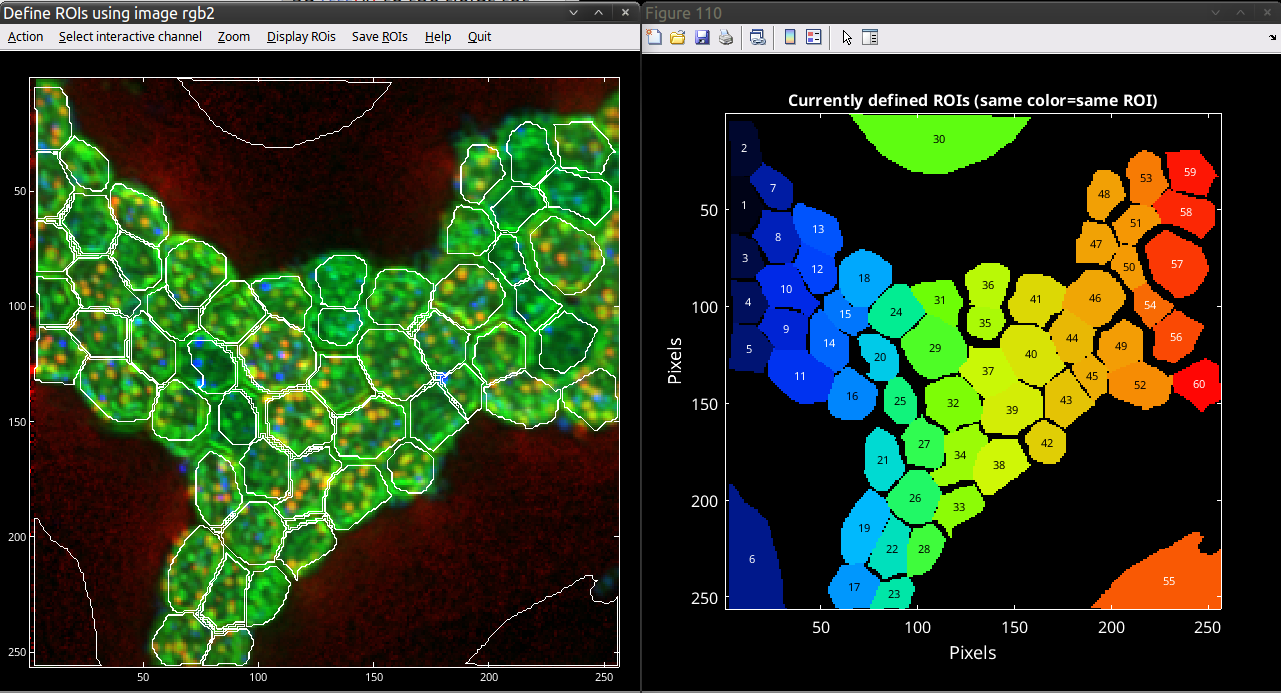
\includegraphics[width=\textwidth]{figs3/LANS-roi-definition-tool}
\caption{\label{fig:roi-definition-tool}%
Definition of regions of interest (ROIs) in LANS. The left window provides tools for manual or semi-automated definition of ROIs, the right window shows the currently defined ROIs. The defined ROIs are displayed as outlines in the left window and colored areas in the right window. Note that the ROIs are numbered such that the ROI's central points increase from left to right. Also note the Help in the menu, where you can learn more details and useful tricks.}
\end{figure}

\setcounter{step}{0}

\s In the ROI definition window, select \lans{Action} $\ra$ \lans{Draw ROIs freehand} (\ttt{Ctrl+d}) to draw a ROI using a mouse.

\bul Click the left mouse button, hold it, and draw a region of interest. 

\bul After releasing the mouse button, you can move the ROI around using a mouse. 

\bul Double-click on the ROI to confirm its final position.

\bul When prompted, specify whether the ROI outline should be defined as the \lans{coarse polygon} you have just drawn or as an \lans{ellipse that circumscribes} this polygon. Typically, you will choose the first option: coarse polygon. At this point, you can also cancel the ROI definition by selecting \lans{Do not take anything}.

\s Experiment with different ways of defining ROIs, such as drawing them as \lans{ellipses} (\ttt{Ctrl+e}) or \lans{rectangles} (\ttt{Ctrl+t}), or via \lans{Interactive thresholding}. In certain situations, the last approach is particularly useful and will be described in greater detail later on.

\bul Remember: after drawing a~ROI, you always need to double-click on it to confirm its size and location.

\bul Note that if you draw a ROI over another, previously defined ROI, the last one will take the priority. In this way, you can draw a~ROI inside a~ROI (but not a~ROI outside a~ROI).

\bul If you click within the ROI outline, the ROI identifier (number) will be displayed in the Matlab console. Note that ROIs are renumbered everytime you add or remove a~ROI, such that the ROIs' central points increase from left to right.

\s Select \lans{Display ROIs} $\ra$ \lans{Display ROIs with ROI ID's} (\ttt{Ctrl+w}) to display the currently defined ROIs.

\bul By default, they will be displayed in a~window placed \bb{just to the right} from the window of the ROIs definition tool (Fig.~\ref{fig:roi-definition-tool}). Thus, it is recommended that you keep the latter window somewhere on the left side of your screen. If you had placed that window near the right edge of your screen, it may happen that the window with the ROIs will be invisible (because it will be placed to the right of the tool window, i.e., outside of your screen).

\bul Notice that ROI identification numbers (IDs) are generated automatically and increase from left to right when sorting the ROIs based on their central point.

\bul If you want to display ROIs with specific IDs, you can do so by typing the IDs in the dialog that opens after you choose to display the ROIs.

\bul If the ROIs have been classified, you can display ROIs from a~specific class by typing the corresponding class identification letter, rather than the ROI identification number, in the same dialog.

\s Explore the \lans{Action} menu to test various ways to \lans{define}, \lans{split}, \lans{merge}, or \lans{remove} ROIs.

\s Use the \lans{Zoom} menu to zoom in the ROI definition image or zoom out.

\bul Note another Matlab-related peculiarity: Once you select \lans{Zoom} $\ra$ \lans{Zoom ENABLE} (\ttt{Ctrl+z}), you \bb{enter} a~`zoom' mode. In this mode, you can use the mouse to specify the zoomed-in area. Subsequently, you must \bb{quit} the `zoom' mode by selecting \lans{Zoom} $\ra$ \lans{Zoom DISABLE} (or pressing \ttt{Ctrl+z} again). Only then can you proceed with other actions.

\s Select \lans{Save ROIs} from the menu, or press \ttt{Ctrl+s}, to save the currently defined ROIs. 

\bul You can choose the default name (e.g., \ttt{ROIs.mat}) or a different name (e.g., \ttt{cells.mat}).

\bul Note that there is \bb{no undo} function implemented in LANS (yet). Thus, it is recommended that you save the ROIs frequently, or at least after you have made an effort to define a~few complicated ROIs that you do not want to loose.

\s When you are satisfied with the defined ROIs, display them all again by selecting \lans{Display ROIs} $\ra$ \lans{Display ROIs with ROI ID's} (\ttt{Ctrl+w}). This will set the floor for the next step: ROI classification.

%%

\subsubsection{ROI definition via interactive thresholding}
\setcounter{step}{0}

Before we continue with ROI classification, we describe an example of how to define ROIs via interactive thresholding. In general, once you get used to it and learn the tricks, this approach allows you to define ROIs more efficiently and reproducibly than by drawing them manually. However, the approach is only applicable if the signal used for recognizing the ROI \bb{stands out} relative to the surrounding background.

In this particular example, you will draw a~ROI that corresponds to a~cyanophycin inclusion inside one of the cells. The inclusion is characterized by a~pronounced enrichment in the ${}^{15}N$ isotope relative to the cell biomass. Because the ${}^{15}N$ atom fraction (i.e., the ratio \ttt{12C15N/(12C14N+12C15N)}) is used as the red channel in the ROI definition template, the inclusion can be recognized as an~orange spot (it contains $CN$ in green, and high ${}^{15}N$ in red).

\s In the ROI definition tool window, zoom in to a group of cells with clear orange spots (e.g., as shown in Fig.~\ref{fig:roi-interactive5}A).

\s Because an RGB overlay is now used as a~ROI definition template, the interactive channel needs to be defined first. As mentioned above, the red channel will be the interactive one in this example. Hence, choose \lans{Select interactive channel} $\ra$ \lans{Red} from the menu. 

\bul This step would not be necessary if only one channel was used as the ROI definition template. 

\bul Note that through the \lans{Select interactive channel} menu, you can also choose which of the RGB channels should be displayed or hidden during ROI definition (compare panels A--D and E in Fig.~\ref{fig:roi-interactive5}). You can do this also more quickly by pressing \ttt{Ctrl+1}, \ttt{Ctrl+2} or \ttt{Ctrl+3} to hide or show the R, G or B channel, respectively.

\begin{figure}[!ht]
\centering
\begin{tabular}{cccccc}
A: \includegraphics[scale=0.23]{figs3/LANS-roi-interactive0}
&
B: \includegraphics[scale=0.23]{figs3/LANS-roi-interactive1}
&
C: \includegraphics[scale=0.23]{figs3/LANS-roi-interactive2}
\\[5mm]
D: \includegraphics[scale=0.23]{figs3/LANS-roi-interactive3}
&
E: \includegraphics[scale=0.23]{figs3/LANS-roi-interactive4}
&
F: \includegraphics[scale=0.23]{figs3/LANS-roi-interactive5}
\end{tabular}
\caption{\label{fig:roi-interactive5}%
ROI definition via the interactive thresholding approach. (A)~A~zoomed-in area in the image, with no ROI yet defined. (B)~A~ROI outline (in white) is drawn automatically by selecting the red channel as the active one, starting the interactive thresholding mode, and clicking on the pixel indicated. The selected area can be enlarged~(C) or made smaller~(D) by repetatively pressing the \ttt{up} or \ttt{down} arrow keys while the interactive thresholding mode is active. The ROI is confirmed by pressing \ttt{Enter}, which will stop the interactive thresholding mode. (E)~Image of the same area but with the green channel hidden from view. (F)~If the green channel, instead of the red one, was selected as the active one, interactive thresholding would draw ROI based on the intensity of the green colour. In this particular case, this approach would not be very useful for defining ROIs corresponding to individual cells, because the cells are not well separated from each other (although they do stand out relative to the background filter). This may be different in other datasets, however, allowing rapid definition of ROIs corresponding to cells.}
\end{figure}

\s Select \lans{Action} $\ra$ \lans{Interactive thresholding} (\ttt{Ctrl+a}) to start ROI definition via interactive thresholding.

\bul Click with a~left-mouse button on the image in a~pixel with a~high signal of the active channel (i.e., somewhere on the orange spot). You will notice that a~ROI outline is automatically drawn (Fig.~\ref{fig:roi-interactive5}B). The outline corresponds to a~contour where the signal values (of the active channel) do not fall below the value in the selected (clicked) pixel multiplied by a~threshold value.

\bul This threshold value is 0.5 by default, but it can be changed interactively by pressing the \lans{up} or \lans{down} arrow key, respectively. When doing so, the ROI outline will cover a~larger (Fig.~\ref{fig:roi-interactive5}C) or smaller (Fig.~\ref{fig:roi-interactive5}D) area. Keep pressing the \lans{up} or \lans{down} arrow key, repetatively but slowly, to observe this behaviour. 

\bul If a~different pixel is selected (clicked), the ROI outline is automatically redrawn according to the current threshold.

\bul By combining left-button mouse clicks with the \lans{up} and \lans{down} arrows, you can rapidly optimize the ROI definition.

\s When you are satisfied with the defined ROI, e.g., if the defined ROI looks as shown in Fig.~\ref{fig:roi-interactive5}D, \bb{press \ttt{Enter} to confirm it}. Press \ttt{Esc} if you want to cancel the current interactive ROI definition.

\bul This is one of the moments when you can get ``stuck'', and become unnecessarily frustrated, if you do not correctly follow the sequence of steps described above. Specifically, \bb{if you start} the \lans{Interactive ROI definition} sequence of actions, \bb{you \emph{must} terminate it} properly by pressing either \ttt{Enter} (confirm the ROI) or \ttt{Esc} (cancel the interactive ROI definition). 

\s At this point, it is recommended that you spend some time practicing the above sequence of steps. Once you get used to it, it can fairly substantially speed up your ROI definition.

\s Note that the interactive thresholding approach is, essentially, an automatic drawing of a~contour at a~particular height on a~\bb{hill}. If you want to apply the same approach but for a~\bb{valley}, you need to convert valleys into hills and vice versa. You can do this by selecting \lans{Action} $\ra$ \lans{Invert template image} (Fig.~\ref{fig:interactive-invert}). When doing so, it will probably be a~good idea to also change the color of the ROI contour line (e.g., from the default \ttt{w}hite to blac\ttt{k}), which you can do by selecting \lans{Action} $\ra$ \lans{Change color of the ROI outline}. Then continue in the same way as described above (steps 3--4) to define a~ROI. You can always get back to the original template by inverting it again.

\begin{figure}[!ht]
\centering
\begin{tabular}{ccc}
A: \includegraphics[scale=0.19]{figs3/LANS-roi-interactive6}
&
B: \includegraphics[scale=0.19]{figs3/LANS-roi-interactive7}
&
C: \includegraphics[scale=0.19]{figs3/LANS-roi-interactive8}
\end{tabular}
\caption{\label{fig:interactive-invert}%
ROI definition via interactive thresholding using the original and inverted template image. (A)~In the original template, a~ROI corresponding to \bb{all cells} on a~filter is defined by following steps 3--4, using \bb{green} channel as the active one. (B)~To define a~ROI corresponding to the \bb{filter} (the upper part), the template image needs to be first inverted. The ROI is then defined following the same procedure, including the same active channel. The defined ROIs will then look as depicted in panel C.}
\end{figure}

%%

\subsection{Classify ROIs}

It is often useful to classify the defined ROIs. It is recommended to classify the ROIs \bb{after} the ROI definition has been fully completed and quality checked. This is because ROI definition, when performed with a~linked ROI classification file, is still not completely bug-free and may lead to a~mismatch between defined and classified ROIs after splitting a~ROI to multiple ROIs.

ROIs can be classified manually or automatically. Here, we focus on manual ROI classification, which is done in most cases. Automatic ROI definition will be explained in Section~\ref{sec:manual_ROI_classification}.

We emphasize that ROI classes in LANS are identified by \bb{single letters} (e.g., \ttt{a}, \ttt{b}, \ttt{A}, \ttt{B}). Upper-case and lower-case letters refer to \emph{different} classes. It is up to the user to keep track of the full class name (e.g., algal cell, bacterial cell, filter) and the corresponding class identifier (e.g., \ttt{a}, \ttt{b}, \ttt{x}). Also, it is not recommended to use a~class identifier \ttt{i}, since this letter is automatically assigned to ROIs inserted to a~previously defined and classified set of ROIs.

\setcounter{step}{0}

\s While having the ROIs displayed, select in the main LANS window \lans{ROIs} $\ra$ \lans{Classify} $\ra$ \lans{ROIs manually (ROI by ROI)}.

\s In the new window that opens (Fig.~\ref{fig:roi-classification}), specify the \lanstf{ROI number} identifying the ROI and the corresponding \bb{letter} identifying the \lanstf{ROI class}, then click \lans{Add/Replace} (or press \ttt{Ctrl+Enter}).

\begin{figure}[!ht]
\centering
\includegraphics[scale=0.4]{figs3/LANS-roi-classification}
\caption{\label{fig:roi-classification}%
LANS window where you can classify ROIs manually.}
\end{figure}

\bul Notice that after you add a~classified ROI, the ROI identifier number is automatically increased by one and the ROI class letter is highlighted. This allows you to simply type in another (or the same) letter and press \ttt{Ctrl+Enter} to classify the subsequent ROI. By repeating this, you can fairly quickly classify many ROIs.

\bul Ensure that you correctly add the \emph{last} ROI to the list of classified ROIs. It often happens that users forget this and end up with one less ROI classified than defined, which causes errors later on.

\s Click on \lans{Save As} to store the ROI classification information in a~file. It is important, but also logical, that the filename (not the extension, see next) is the same as the name of the ROI definition file. For example: if ROIs are stored in \ttt{ROIs.mat} or \ttt{cells.mat}, the corresponding classes should be stored in \ttt{ROIs.dat} or \ttt{cells.dat}, respectively.

\s Revise the ROI classification. If you need to change ROI's class, click on the ROI identifier number, change its class, and click on \lans{Add/Replace} (or press \ttt{Ctrl+Enter}) to update it.

\s Click on \lans{Save} to store the ROI classes in the same file as defined via \lans{Save As} (Step~3).

\s Close the ROI definition and ROI classification windows when finished with the definition and classification tasks.

%%

\subsection{Display and export ROI-specific data}
\setcounter{step}{0}

\s Ensure that ROIs have been defined and, if required, classified.

\bul If ROIs have been defined in an earlier LANS session, you first need to load them via \lans{ROIs} $\ra$ \lans{Load ROIs from disk} in the main LANS window.

\s Check \lanscb{Plot x-y-z graph} in the \ttt{Output options} box and type identifiers (1--8) of the masses or ratios that you want to include in a~scatter plot in the \lanstf{R/x}, \lanstf{G/y} and \lanstf{B/z} fields (Fig.~\ref{fig:scatter-plots}).

\begin{figure}[!ht]
\centering
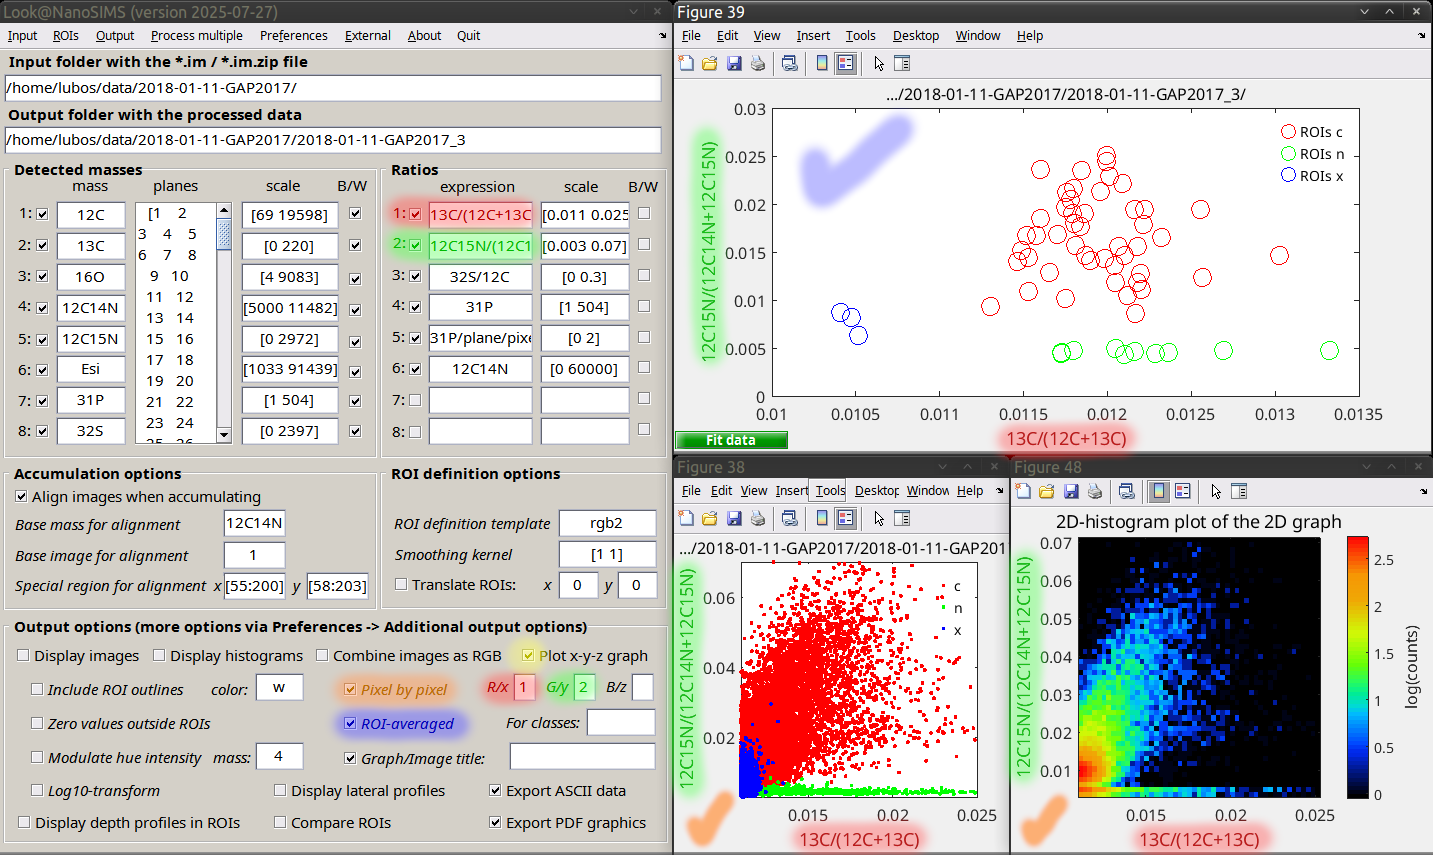
\includegraphics[width=0.9\textwidth]{figs3/LANS-scatter-plots}
\caption{\label{fig:scatter-plots}%
Examples of 2D scatter plots generated by LANS. They can show ROI-averaged values (blue) or pixel-by-pixel values (orange).}
\end{figure}
 

\bul If all three fields are filled in, the ROI-specific values will be plotted in a~3D scatter plot (x--y--z). If only two of the three fields are filled in, a~2D scatter plot (x--y) will be created.

\bul In the \ttt{Ratios} or \ttt{Detected masses} box, ensure that the checkboxes corresponding to the identifiers filled in the \lanstf{R/x}, \lanstf{G/y} and \lanstf{B/z} fields are checked, too. 

\s Check \lanscb{ROI-averaged} or \lanscb{Pixel by pixel} (also in the \ttt{Output options} box; Fig.~\ref{fig:scatter-plots}) if you want to display a~scatter plot for ROI-specific or pixel-specific values, respectively.

\bul You can have both of them checked at the same time. 

\s Check \lanscb{Export ASCII data} and \lanscb{Export PDF graphics} to ensure that the data and graphs will be exported (in the \ttt{dat} and \ttt{pdf} sub-folders of the dataset folder, respectively).

\s When plotting scatter plots, it is typically not necessary anymore to display the corresponding images. If this is the case for you, uncheck the \lanscb{Display images} checkbox.

\s Select \lans{Output} $\ra$ \lans{Display masses} or \lans{Display ratios} to \bb{create scatter plots} of the ROI-specific or pixel-specific values of the desired quantities and \bb{export the values and graphs}. 

\bul In the process, you will be prompted to select a~ROI classification file. If the file exists (and it is up-to-date), select it. In this case, different colors will be used to mark ROI from different classes (Fig.~\ref{fig:scatter-plots}). 

\bul If the ROI classification file does not exist, click \ttt{Cancel} or press \ttt{Esc} when prompted for the file. In this case, all ROIs will be treated equally and displayed in one color.

\bul If you only want to display values for specific classes, you can enter the identifiers for those classes in the \lanstf{For classes} field (just below the R/x, G/y and B/z fields) first, then select \lans{Output} $\ra$ \lans{Display masses} or \lans{Display ratios}.

\bul If you choose to display ROI-specific values, it is possible to add a~ROI identifier and an~error-bar to each data point. This is achieved by selecting the corresponding options via \lans{Preferences} $\ra$ \lans{Additional output options}. The error-bar size will indicate the Poisson error, derived from the total ion counts per ROI.

\bul The output data and images will be stored in the \ttt{dat} and \ttt{pdf} sub-folders of the dataset folder, respectively. Formatting of the data output is self-explanatory based on the first two lines in the output file.

\s Select \lans{Output} $\ra$ \lans{Check output consistency} to check that the exported ROI-specific data are consistent with the defined ROI  classes (only relevant if working with classified ROIs). 

\bul More specifically, the output is consistent if the number of defined ROIs, the number of classified ROIs, and the number of ROIs for which the ROI-specific data have been exported, is the \emph{same}.

\bul Output inconsistency can occur if, e.g., you redefine ROis but forget to reclassify them or reexport the ROI-specific data (or any combination of these three actions).

\bul When prompted, select the ROI classification file and view the results of the consistency check in the Matlab console. 

\bul If any of the output lines does not contain \ttt{OK}, you should revise your analysis by reclassifying the ROIs or reexporting the ROI-specific data for the affected variables.

%%

\subsection{Display depth profiles in ROIs}
\setcounter{step}{0}

NanoSIMS measurements are conducted by sputtering away the sample material in multiple scans over the same field of view while collecting the secondary ions. The resulting image stack therefore reflects elemental and isotopic distribution of the sample along the vertical dimension. You can display and export this vertical (depth) variation in ROIs using the following steps.

\s Ensure that ROIs have been defined or loaded into the current LANS session.

\s Check \lanscb{Display depth profiles in ROIs} in the \ttt{Output options} box.

\bul Typically, you will want to uncheck all other checkboxes in the \ttt{Output options} box to prevent cluttering of your screen with too many figures.

\s Check \lanscb{Detected masses} or \lanscb{Ratios} for which you want to display the depth profiles.

\s Select \lans{Output} $\ra$ \lans{Display masses} or \lans{Display ratios}.

\bul Observe the output in the Matlab console, which informs you about significant trends with depth of the particular mass or ratio in ROIs.

\bul In the process, the depth profiles are exported in data files with an extension \ttt{dap} (located in the \ttt{dat} sub-folder of the dataset folder).

\s In the new window that opens, select ROI identifiers for which you want to display the depth profiles. Then, select the mass or ratio in the list to display the depth profiles in the selected ROIs (Fig.~\ref{fig:depth-profiles}).

\begin{figure}[!ht]
\centering
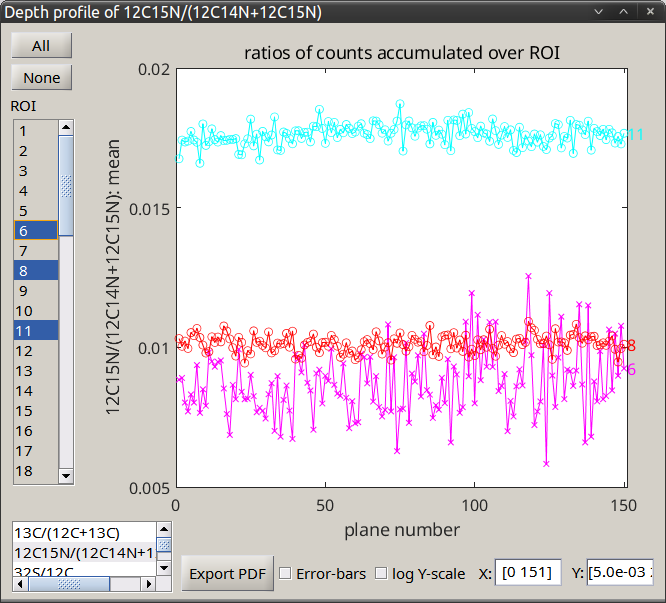
\includegraphics[scale=0.4]{figs3/LANS-depth-profiles}
\caption{\label{fig:depth-profiles}%
Using LANS to display depth profiles of ion counts and ion count ratios in ROIs.}
\end{figure}

\s Select \lans{Export depth profile} to export the graph with depth profiles in the currently selected ROIs.

%%

\subsection{Finalize the processing of an individual dataset}
\label{sec:final-steps}
\setcounter{step}{0}

If you want to reprocess a~particular dataset in the future and start the processing from the same stage where you finished, you will need to have the data processing settings stored. If you want to share or communicate the results with collaborators, a~graphical output where all the images and graphs generated by LANS are nicely assembled might be a~good idea. Finally, if you want to make a~backup of the processed data for yourself or for sharing with collaborators, having a~compressed version of the processed data folder would probably be the best approach. You can generate these types of output quickly and efficiently within LANS using the following steps:

\s Select \lans{Output} $\ra$ \lans{Generate LaTeX + PDF output} to export results of your analysis in a~PDF document (example shown in Fig.~\ref{fig:outputG}). 

\bul Before you do this, slecect checkboxes in the \ttt{Output options} box to specify which kind of results you want to have included in the graphical output, such as  \lanscb{images}, \lanscb{scatter plots}, \lanscb{RGB overlays}, \lanscb{histograms}, \lanscb{depth profiles}, etc.

\bul If you check \lanscb{View PDF after export} (available via \lans{Preferences} $\ra$ \lans{Additional output options}) and correctly set the full path to a~PDF viewer in the \ttt{PDF\_VIEWER} variable (this variable is defined in the \ttt{lans\_paths.m} file), the PDF output will automatically be displayed after it has been generated. This can be convenient if you want to see the results quickly, without the need for browsing through the different folders on your computer.

\begin{figure}[!ht]
\centering
\begin{tabular}{ccc}
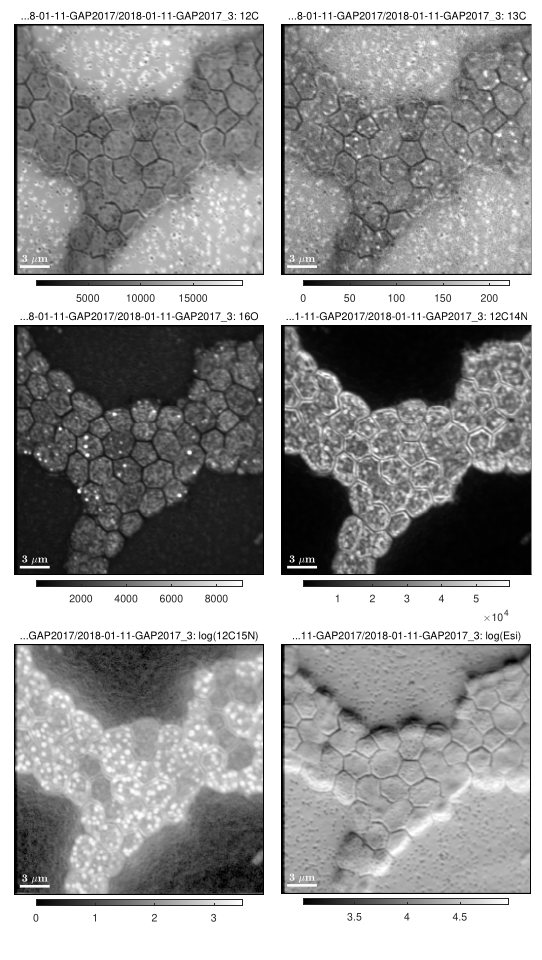
\includegraphics[width=0.31\textwidth, valign=t]{figs3/outputG1}
&
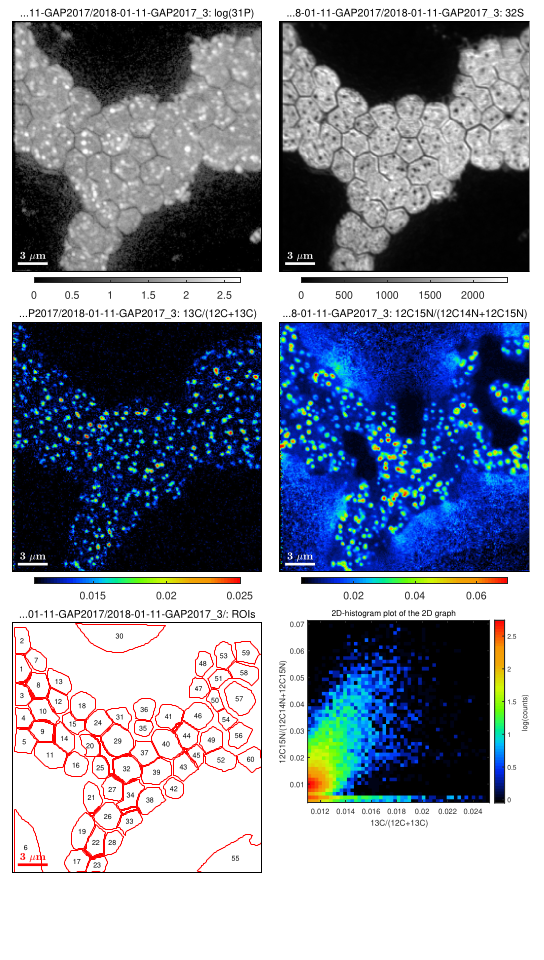
\includegraphics[width=0.31\textwidth, valign=t]{figs3/outputG2}
&
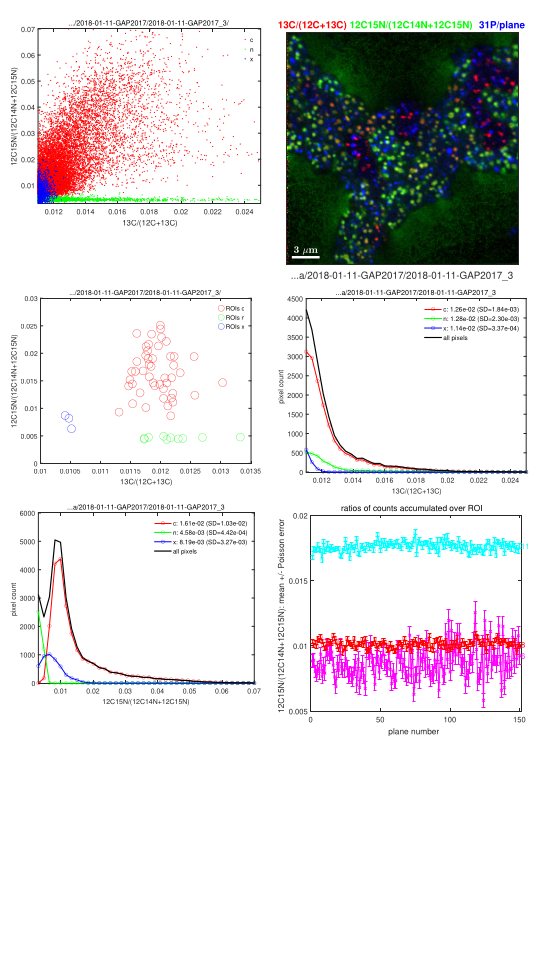
\includegraphics[width=0.31\textwidth, valign=t]{figs3/outputG3}
\end{tabular}
\caption{\label{fig:outputG}%
Example of the first three pages in the graphical output generated at the end of processing of an individual dataset with LANS.}
\end{figure}

\s Select \lans{Preferences} $\ra$ \lans{Store preferences} to save the settings of the current data processing session in a file (it is recommended to use the file name \ttt{prefs.mat}). 

\bul This is useful when you want to return to the analysis of the same file in the future, but also if you want to later combine results of your analyses of multiple datasets via ``metafile processing'', as described in Section~\ref{sec:level2}. Therefore, it is highly recommended that you do this for every processed dataset.

\bul More specifically, the preferences file will contain all information for the currently processed dataset that you see in the main LANS window, including the names of detected masses, planes selected for alignment, formulas for ion count ratios, scales for mass and ratio images, output options, etc.

\s Select \lans{Preferences} $\ra$ \lans{Backup (full) folder with processed data}.

\bul This will compress the \emph{entire} content of the processed data folder in a~\ttt{zip} file.

\bul Additionally, a~copy of the PDF output file will be created and renamed to match the name of the processed data.

\s Alternatively, select \lans{Preferences} $\ra$ \lans{Backup (minimal) folder with processed data}.

\bul This will only compress the \emph{minimal} information in the processed data folder, based on which the rest of the processed data can easily and reproducibly be generated by repeating the processing steps in LANS. 

\bul This minimal information includes the preferences (e.g., \ttt{prefs.mat}), plane alignment information (\ttt{xyalign.mat}), ROI definition (e.g., \ttt{ROIs.mat}), and ROI classification (e.g., \ttt{ROIs.dat}).

%\section{Analysis of multiple datasets --- ``metafile processing''}
\label{sec:level2}

\purplebox{}
It is assumed that you have processed multiple NanoSIMS datasets using steps described in Section~\ref{sec:level1}, which left you with output such as isotope ratio values and images scatterred across \bb{multiple} files and folders, organized as described in Section~\ref{sec:data_organization}. This section explains how to quickly \bb{merge} these multiple files into \bb{one} output. This output, and in particular the isotope ratio values exported in a~text format, can be used for further, more sophisticated analyses (e.g., statistical analysis) by other, third-party software. If you are a~skilled data analyst, you can arguably do this more efficiently by creating scripts in a~programming language of your choice. This section describes how to do this in LANS, if your coding abilities are more limited.
\tcbe

As an example, we will use processed data for four datasets, each corresponding to cyanobacterial cells incubated under different experimental conditions (treatments): 
\begin{itemize}
\item[--]\ttt{2018-01-05-GAP2017\_1} (treatment~0)
\item[--]\ttt{2018-01-05-GAP2017\_2} (treatment~1)
\item[--]\ttt{2018-01-11-GAP2017\ 3} (treatment~2)
\item[--]\ttt{2018-01-11-GAP2017\_5} (treatment~3)
\end{itemize}
The datasets and the corresponding folders containing the processed data (backed up in \ttt{zip} files, as described in Section~\ref{sec:final-steps}, step~3) are available in the same location as the LANS program (folder \ttt{test\_data/GAP2017}). It is recommended that you check these data before you continue with the metafile processing steps described in this section.

%%%%

\subsection{Generate a metafile}
\setcounter{step}{0}

\goldbox{}
The first step involves the definition of a~list of datasets and variables that you want to merge and analyze together. In the context of LANS, this list is stored in a~so-called \bb{metafile}, which is a~simple text file containing the required information including the absolute path to the processed data structure, relative paths for the individual datasets, and variables of interest (see below, step~10). This file can be generated in a~simple text editor, but it is better to start using a~dedicated tool in LANS to avoid syntax or formatting errors.
\tcbe

\s{Back in the main LANS window, select \lans{Process multiple} $\ra$ \lans{Generate metafile} to open a~new tool window dedicated to metafile definition (Fig.~\ref{fig:metafile-definition}). }

\begin{figure}[!ht]
\centering
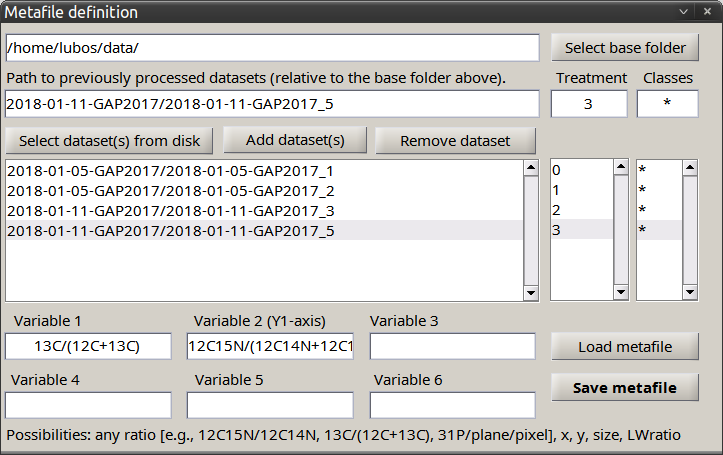
\includegraphics[scale=0.5]{figs3/LANS-metafile-definition}
\caption{\label{fig:metafile-definition}%
LANS tool for defining a~metafile.}
\end{figure}

\sbx{In this window, click on \lans{Select base folder} to select the absolute path to the processed datasets.}

\nb{It is assumed that the folders with the processed datasets are located in this path or in sub-folders under it.}

\sbx{Click on \lans{Select dataset(s) from disk}, navigate to a~specific processed dataset, and select it.}

\nb{You need to select the raw data file (\ttt{im} or \ttt{im.zip} file), not the sub-folder containing the processed data. However, the corresponding sub-folder with the processed data \bb{must} exist.}

\nnb{You can select multiple datasets at once by holding the \ttt{Ctrl} key while selecting the files.}

\nnb{You can also select the \ttt{prefs.mat} file corresponding to the raw dataset. If you processed the dataset and stored the preferences at the end of processing, as emphasized in Section~\ref{sec:final-steps}, step~2, this file will be present in the dataset folder.}

\sbx{Enter a~\lanstf{treatment identifier} to the provided field.}

\nb{This must be an \bb{integer number}, e.g., $0$ for a~control treatment, $1$ for treatment~1, etc.}

\nnb{It is up to you to keep track of the correspondence between the treatment identifiers and the true meaning of the treatments.}

\sbx{Enter \lanstf{ROI classes} to the provided field.}

\nb{Enter \ttt{*} if you want to analyze \bb{all} ROI classes, unless you really only want to analyze ROIs from a~specific class. Note that you will be able to make this selection later on anyway, so it is best to simply enter \ttt{*} (as shown in Fig.~\ref{fig:metafile-definition}).}

\sbx{Click \lans{Add dataset(s)} to add the dataset(s) to the list. }

\sbx{Repeat steps S3--S6 to select all datasets that should be part of the metafile processing.}

\sbx{If you want to remove a dataset from the list, select it in the list and then click \lans{Remove dataset}.}

\sbx{In the fields provided, enter \lanstf{variables} that you want to analyze via metafile processing. }

\nb{Ensure that you type the strings \bb{exactly} in the same way as you did during the processing of individual datasets (e.g., \ttt{13C/12C}, \ttt{13C/(12C+13C)}, \ttt{12C15N/12C14N}, \ttt{31P/plane/pixel}, etc.). Best is to copy and paste the strings from the main LANS window to avoid typos.}

\nnb{You can analyze up to six variable simultaneously. The idea behind this limit is that you can, later on, plot the variables against each other in up to three 2D-scatter plots or up to two 3D-scatter plots. Thus, it is good to think ahead and enter the variables in the order how you want to plot them later on. If you only want to plot one variable against another one, e.g., \ttt{13C/12C} on the $x$~axis and \ttt{12C15N/12C14N} on the $y$~axis, enter these expressions into the boxes for \lanstf{variable~1} and \lanstf{variable~2}, respectively, and leave the others empty.}

\sbx{Click \lans{Save metafile} and define the name and location for the metafile.}

\nb{Ideally, to keep everything well organized, the metafile should be located in the \lanstf{base folder} selected above. }

\nnb{For example, if you call the metafile \ttt{m1.txt}, any output generated during processing of this metafile will be stored in a~sub-folder called \ttt{m1}.}

\s{Optionally, explore the content of the metafile by opening it in a~simple text editor (e.g., \ttt{notepad} or \ttt{notepad++}).}

\nb{This is recommended because, later on, you may find it easier to edit the content of this file (e.g., add or remove datasets, modify the variables) directly in the editor rather than through steps S2--S8 described above. An example of the metafile content is shown here:
\begin{center}
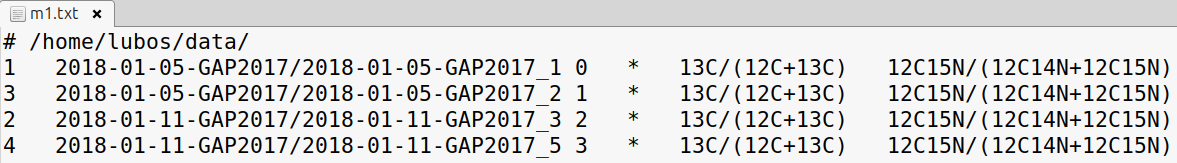
\includegraphics[scale=0.35]{figs3/LANS-metafile-m1}
\end{center}}

%%

\subsection{Metafile processing}
\setcounter{step}{0}

\goldbox{}
First, we describe steps that are common for different types of metafile processing analysis available in LANS. Subsequent steps depend on the particular analysis you want to perform and are described in separate sections below.
\tcbe

\s{Ensure that the metafile is defined and the sub-folders and corresponding output files exist and are consistent for all datasets listed in the metafile.}

\nb{This should be the case if you conducted the data processing attentively and in accordance with instructions described in Section~\ref{sec:level1}. If there are inconsistencies or errors, they will be reported later on in the console (see below).}

\s{Back in the main LANS window, select \lans{Process multiple} $\ra$ \lans{Process metafile} to open a~new tool window dedicated to metafile processing (Fig.~\ref{fig:process-metafile}).}

\begin{figure}[!ht]
\centering
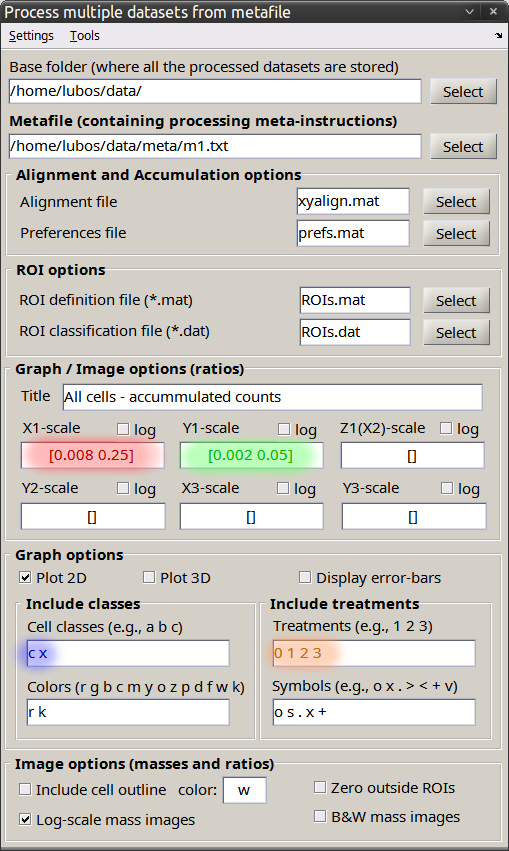
\includegraphics[scale=0.5]{figs3/LANS-process-metafile}
\caption{\label{fig:process-metafile}%
LANS tool for processing a~metafile. If the scale of the variable is specified (highlighted in red and green), it will be applied in the subsequent analyses. An empty scale (\ttt{[]}) will have no effect. In the areas highlighted by blue and orange, you can specify the ROI classes and treatments that should be displayed in the scatter plots, respectively.}
\end{figure}

\sbx{In this window, select the \lanstf{base folder}.}

\nb{Typically, this folder will be the same as specified during metafile definition. However, if you reorganized the data on your computer, or if you conduct the metafile processing on a~different computer, the data organization may be quite different. Thus, this feature makes the metafile processing portable across different computers or differently organized datasets.}

\sbx{Select the \lanstf{metafile}.}

\sbx{Specify  the \lanstf{scale}, separately for each variable.}

\nb{If specified in the form of \ttt{[min max]}, corresponding to a~minimum and maximum value, the scale will be applied during the following analyses. For example, images for the corresponding variable will be reexported as PDF using this new scale, or scatter plots containing the variable will apply this new scale.}

\nb{However, since the optimal scale for the images or graphs may initially be unknown, it is a~good idea to start with an \bb{empty} scale, indicated by \ttt{[]}. This will have no effect on the displayed graphs or images for the corresponding variable.}

\sbx{Check \lanscb{log} if you want to display log-transformed variables.}

\nnb{This can be done separately for each variable.}

\s{Specify the mapping between ROI classes and \lanstf{colors} and between treatments and \lanstf{symbols} in the respective fields. }

\nnb{This mapping will be applied when plotting scatter plots.}

\nb{Colors and symbols recognized by Matlab are already listed between the parentheses (e.g., colors: \ttt{r} for red, \ttt{g} for green, \ttt{b} for blue, \ttt{k} for black, etc., symbols: \ttt{o} for circles, \ttt{s} for squares, \ttt{x} for crosses, \ttt{.} for points, etc.).}

\sbx{Save the metafile processing settings using \lans{Settings} $\ra$ \lans{Save settings}.}

\nnb{This is useful if you plan to return to the same metafile processing session in the future.}

\nnb{Previously saved settings can be loaded using \lans{Settings} $\ra$ \lans{Load settings}.}

\nnb{Now you are ready to continue with \bb{different types} of metafile processing analyses, using steps described in the following sections.}

\subsubsection{Export images for selected variables}
\label{sec:621}
\setcounter{step}{0}

\goldbox{}
This section describes how to merge \bb{images} from multiple datasets into one graphical output (PDF), separately for each variable in the metafile (example shown in Fig.~\ref{fig:metafile-images}). This output is useful for quality checking of ROI definitions and visual assessment or comparative analysis of ion count and ratio images.
\tcbe

\sbx{In the Process metafile window, enter the \lanstf{ROI definition file} in the corresponding field.}

\nnb{This is only relevant if you want to include ROIs in reexported images.}

\nb{It is important that the ROI definition files have the \bb{same name} for \bb{all} datasets in the metafile (e.g., \ttt{ROIs.mat} or \ttt{cells.mat}). If this is not the case, you will need to fix this (simply by renaming the files in the folders for the individual datasets) before proceeding.}

\sbx{Select \lans{Tools} $\ra$ \lans{Export images for each variable as PDF}, or press \ttt{Ctrl+m}. }

\nb{This step will combine images of the variables from multiple datasets and export them in a~PDF output, \bb{one file per variable}, allowing you to view all images from a~specific project at once.}

\nb{The visual comparison of images can be made easier if all images are displayed in the same scale. This is achieved by setting the minimum and maximum values in the corresponding \lanstf{scale} field, as explained above. If you specify the scale, formatted as \ttt{[min max]}, all images of the corresponding variable will be reexported as PDF using the new scale (Fig.~\ref{fig:process-metafile}). If you do not want to reexport the images (e.g., because you have already done so earlier), you need to set the corresponding scale back to \ttt{[]} (i.e., an empty vector).}

\nnb{When doing this, you can use the \lanscb{log} checkbox to set whether a~log-transformed data should be displayed, or the \lanscb{Include ROI outlines} checkbox to set whether the ROI outlines should be included. For the ROI outlines, you can also specify their \lanstf{color} in the corresponding field (e.g., \ttt{w} for white) (Fig.~\ref{fig:process-metafile}). }

\sbx{Observe the console for possible error messages, which are issued if a~particular file is missing.}

\nnb{It may be that there is a~typo in the metafile, or that you forgot to export the variable for a~particular dataset. If this is the case, you will need to reanalyze that dataset and fix the issue.}

\sbx{Observe the console to see the exact locations of the output created by this action.}

\nnb{For example, if your metafile is called \ttt{m1.txt} and the variables of interest include \ttt{13C/(12C+13C)} and \ttt{12C15N/(12C14N+12C15N)}, the images will be exported in files called \ttt{13C-(12C+13C).pdf} and \ttt{12C15N-(12C14N+12C15N).pdf}, respectively, located in the sub-folder \ttt{m1} of the \lanstf{base folder}.}

\nb{Note that the use of \ttt{-} in place of \ttt{/} is necessary because the latter symbol is reserved as a~folder separator in the absolute path to files.}

\nnb{Example of the output generated by these steps is shown in Fig.~\ref{fig:metafile-images}.}

\begin{figure}[!ht]
\centering
\begin{tabular}{cc}
(A) & (B) \\
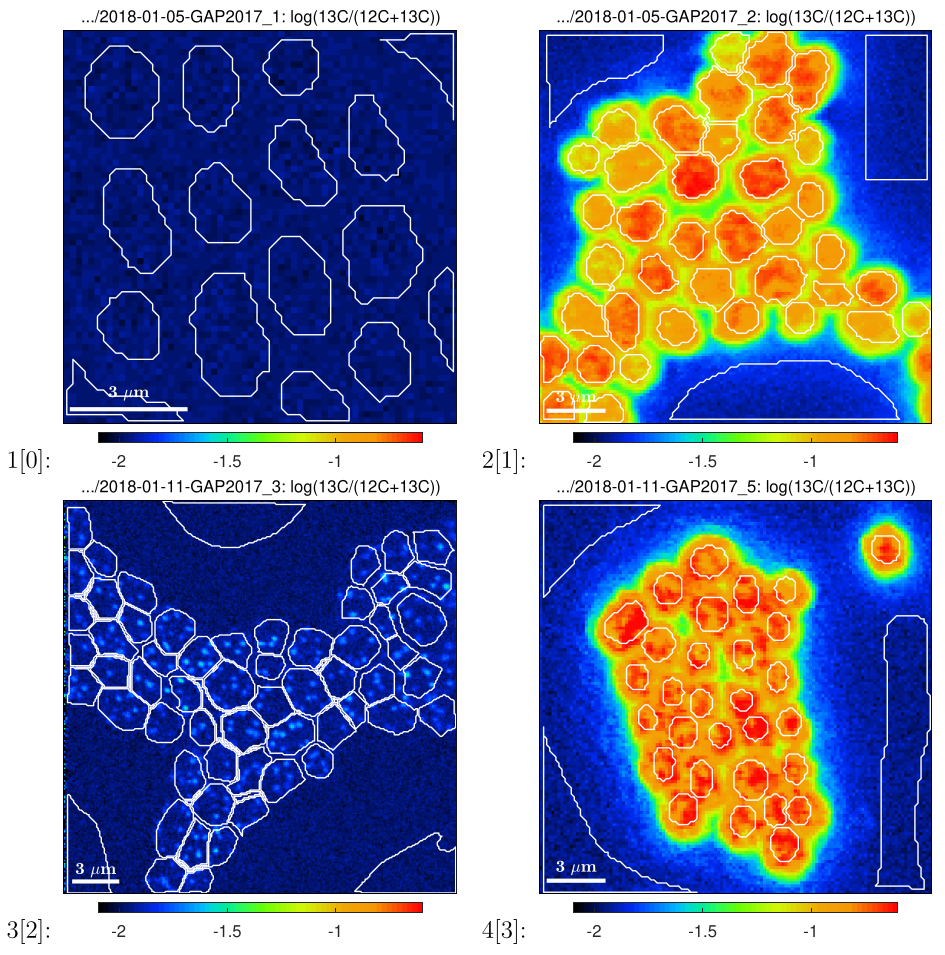
\includegraphics[width=0.47\textwidth, valign=t]{figs3/log(13C-(12C+13C))}
&
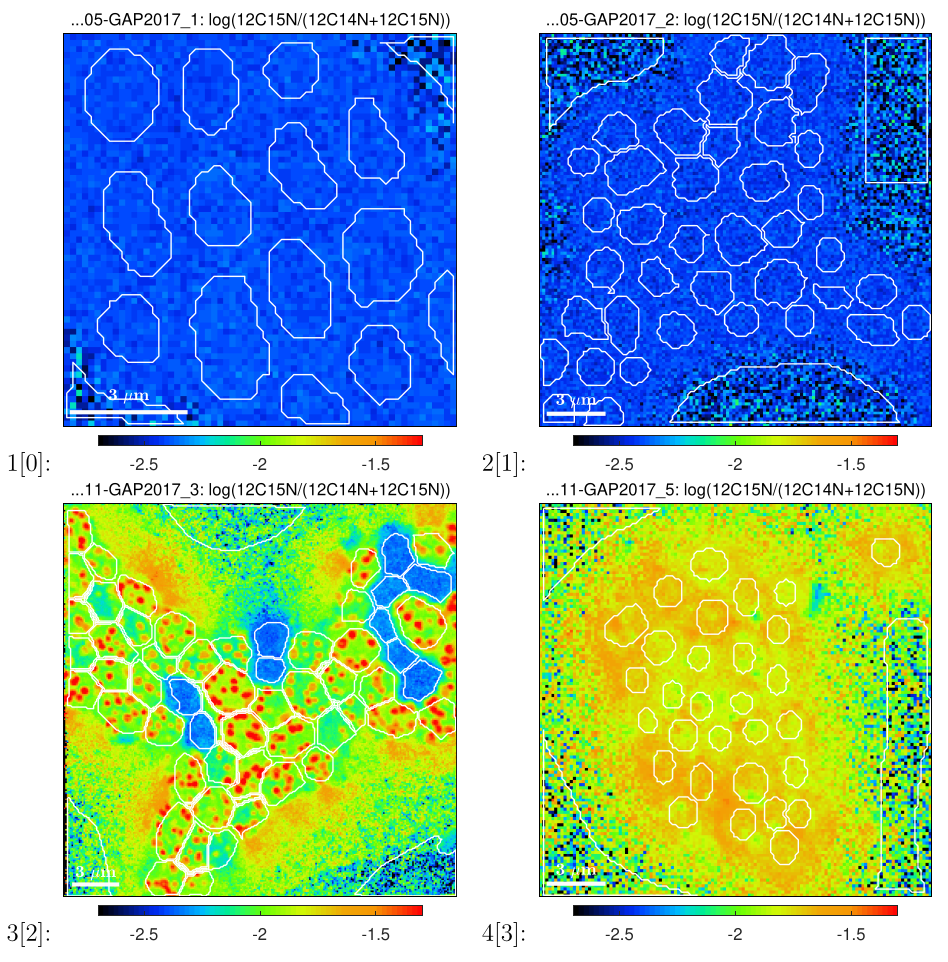
\includegraphics[width=0.47\textwidth, valign=t]{figs3/log(12C15N-(12C14N+12C15N))}
\end{tabular}
\caption{\label{fig:metafile-images}%
Example of the output generated by metafile processing. Shown are (A) \ttt{13C/(12C+13C)} and (B) \ttt{12C15N/(12C14N+12C15N)} ratio images for four datasets. ROI outlines corresponding to individual cells are included, allowing you to quality-check the ROI definition across all datasets. Images have been log-transformed to allow simultaneous visualization of low and high values. All images for a~particular variable are shown in the same scale to aid visual comparison among treatments. The treatment identifiers are shown between brackets ([0--3]) at the bottom-left of each image.}
\end{figure}

%%%%

\subsubsection{Export ROI-specific data for selected variables}
\label{sec:622}
\setcounter{step}{0}

\goldbox{}
This section describes how to merge \bb{text output} from multiple datasets into one data file. The output contains ROI-specific information generated by the analyses of individual datasets, including values of ion counts and ion count ratios, Poisson errors, ROI positions, sizes and classes, and treatment identifiers. This type of information can further be analyzed by statistical tools offerred by LANS (see next section) and beyond.
\tcbe

\sbx{In the Process metafile window, enter the \lanstf{ROI definition file} in the corresponding field.}

\nb{It is important that the ROI definition files have the \emph{same name} for \emph{all} datasets in the metafile (e.g., \ttt{ROIs.mat} or \ttt{cells.mat}). If this is not the case, you will need to fix this (simply by renaming the files in the folders for the individual datasets) before proceeding.}

\sbx{Enter the \lanstf{ROI classification file} in the corresponding field.}

\nnb{This is only relevant if you want to plot ROIs from different classes in different colors.}

\nnb{Similar to the ROI definition files, the ROI classification files must have the \emph{same name} for \emph{all} datasets in the metafile (e.g., \ttt{ROIs.dat} or \ttt{cells.dat}). If this is not the case, you will need to fix this (simply by renaming the files in the folders for the individual datasets) before proceeding.}

\s{Select checkboxes in the \ttt{Graph options} box to specify whether you want to plot a~\lanscb{2D} scatter plot or a~\lanscb{3D} scatter plot, or whether you want to include \lanscb{error-bars} for each data-point.}

\nnb{When plotting 2D scatter plots, 2, 4 or 6 variables must be specified in the metafile. When plotting 3D scatter plots, 3 or 6 variables must be specified in the metafile. It is logical, but it is also useful to emphasize it here.}

\nnb{When including error-bars, their \emph{size} (length) corresponds to the Poisson error.}

\sbx{Select \lans{Tools} $\ra$ \lans{Export and display data in ROIs} $\ra$ \lans{For all datasets in one graph}, or press \ttt{Ctrl+p}.}

\purplebox{}
This step will \bb{merge} ROI-specific data, such as ion counts or ion count ratios, from \bb{multiple} datasets and export the results in \bb{one} data file (with an~extension \ttt{dac}). This file is probably the most useful output for your project, if the project conclusions are drawn from ROI-specific data derived from the analysis of multiple NanoSIMS datasets.
\tcbe

\nnb{In addition to merging and exporting the data, this step will also \bb{plot} the ROI-specific values in a~scatter plot (2D or 3D), using different colors and symbols for different ROI classes and treatments (Fig.~\ref{fig:metafile-scatterplot}).}

\begin{figure}[!hb]
\centering
\begin{tabular}{cc}
(A) & (B) \\
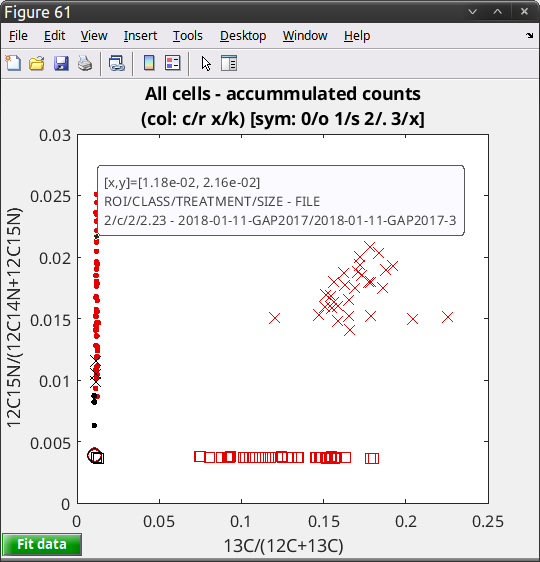
\includegraphics[width=0.44\textwidth, valign=t]{figs3/LANS-metafile-scatterplot1}
&
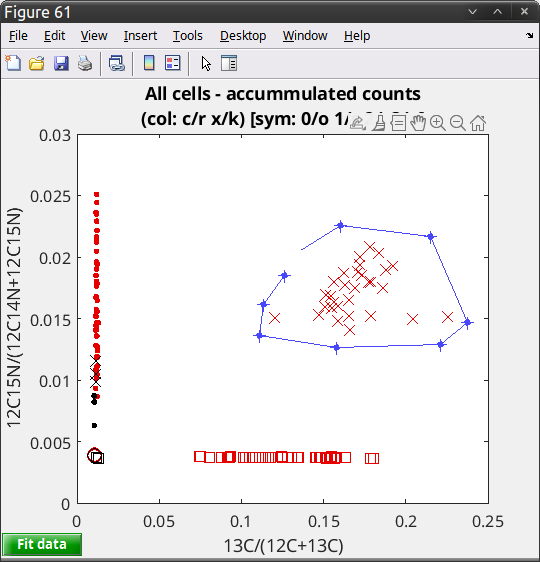
\includegraphics[width=0.44\textwidth, valign=t]{figs3/LANS-metafile-scatterplot2}
\end{tabular}
\caption{\label{fig:metafile-scatterplot}%
Example of a~scatter plot generated by metafile processing.  The plot shows data from four datasets, each corresponding to a~different treatment. (A) By clicking on a~particular data point, you can quickly view relevant information about the data point and thus trace it to a~particular dataset. (B) By clicking on the \lans{Fit data} button, you can manually select a~set of data points (by enclosing them in a~polygon) and analyse them using various types of statistical analyses, including linear regression. }
\end{figure}

\nb{This scatter plot allows you to quickly assess the ROI-specific data visually. It also offers several useful functions to check the data quality and consistency. For example, if you \bb{click} with a~mouse on a~particular \bb{data point}, an annotation will appear providing relevant information about the data point (e.g., the source dataset, ROI identifier, ROI class; Fig.~\ref{fig:metafile-scatterplot}A). You can also click on the \lans{Fit data} button to quickly perform various types of basic statistical analyses on manually selected data points, including linear regression (Fig.~\ref{fig:metafile-scatterplot}B).}

\sbx{When merging data from multiple datasets, observe the console for possible error messages, which are issued if a~particular file is missing.}

\nnb{It may be that there is a~typo in the metafile, or that you forgot to export the data for a~particular dataset. If this is the case, you will need to reanalyze that dataset and fix the issue.}

\sbx{Observe the console to see the exact locations of the output created by this action.}

\nnb{For example, if your metafile is called \ttt{m1.txt} and the variables of interest include \ttt{13C/(12C+13C)} and \ttt{12C15N/(12C14N+12C15N)}, the ROI-specific data will be exported in the file called \ttt{m1.dac} and the scatter plot will be exported in the file called \ttt{m1-13C-(12C+13C)--12C15N-(12C14N+12C15N)-all.pdf}, both located in the sub-folder \ttt{m1} of the \lanstf{base folder}.}

%%

\subsubsection{Basic statistical analysis}

\goldbox{}
Statistical analysis of ROI-specific data for a particular project can be done by third-party tools using the text output generated as described in the previous section.  However, if your statistical knowledge and skills are limited, you can perform some \bb{basic} analyses in LANS, such as calculating group means and standard deviations or comparing means among groups (ROI classes or treatments). The following steps describe how to do this via metafile processing in LANS.
\tcbe

\noindent
The initial 2 steps are the same as those described in the previous section and will not be repeated here.

\setcounter{step}{2}
\sbx{Select \lans{Tools} $\ra$ \lans{Compare classes and treatments}, or press \ttt{Ctrl+e}.}

\nnb{This step will merge ROI-specific data from multiple datasets and pass the output to a~tool that allows you to perform the statistical analysis (Fig.~\ref{fig:lans-statistics}).}

\begin{figure}[!ht]
\centering
\begin{tabular}{c@{\hskip2mm}c}
(A) & (B) \\
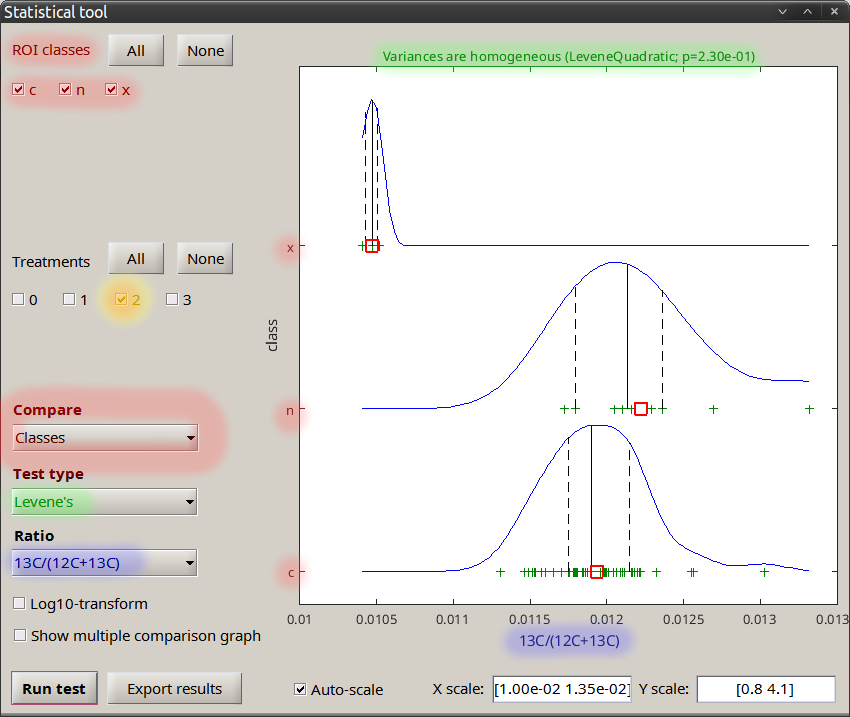
\includegraphics[width=0.475\textwidth, valign=t]{figs3/LANS-statistics1}
&
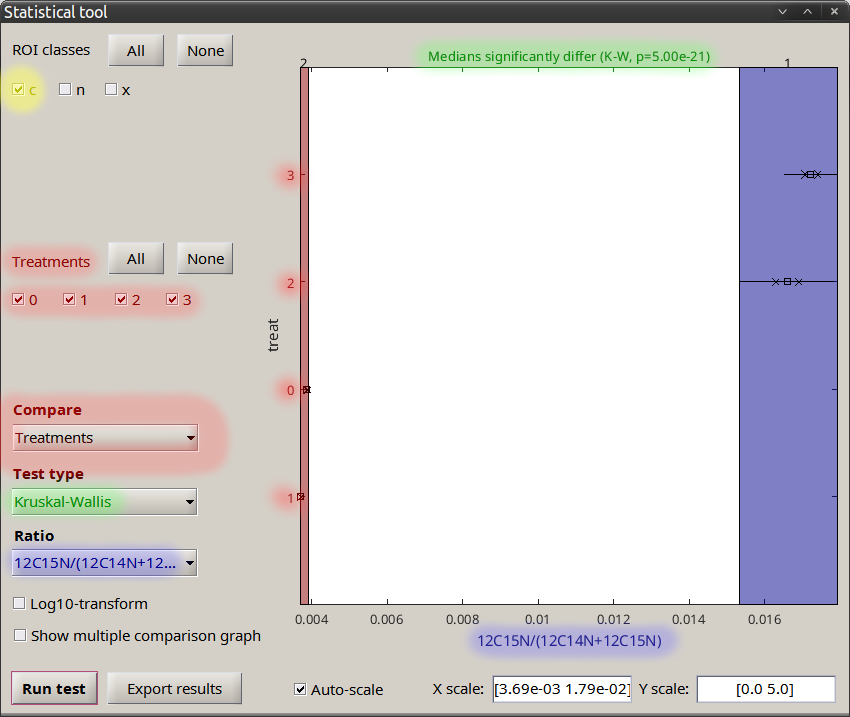
\includegraphics[width=0.475\textwidth, valign=t]{figs3/LANS-statistics2}
\end{tabular}
\caption{\label{fig:lans-statistics}%
Examples of basic statistical tests that you can perform in LANS. (A) Comparison of multiple classes for one treatment. (B) Comparison of multiple treatments for one class. Note the relationships between the fields highlighted in the same color.}
\end{figure}

\s{Select multiple checkboxes for the \lanscb{ROI classes}, then select one checkbox for the \lanscb{Treatment} of interest,  and then select \lans{Compare} $\ra$ \lans{Classes} (Fig.~\ref{fig:lans-statistics}A).}

\nnb{This selection will allow you to compare values across multiple ROI classes for one specific treatment.}

\sbx{Select the \lans{Test type} and the \lans{Ratio} you want to analyze.}

\nnb{For example, by selecting Levene's test and \ttt{13C/(12C+13C)}, you will be able to test for the homogeneity of variance in the ${}^{13}C$ atom fractions.}

\sbx{Click on \lans{Run test} to perform the analysis. }

\nnb{Results will be displayed in the graph (Fig.~\ref{fig:lans-statistics}A) and also in the Matlab console.}

\sbx{Click on \lans{Export results} to export the results as text and graphics.}

%%

\s{Select multiple checkboxes for the \lanscb{Treatments}, then select one checkbox for the \lanscb{ROI class} of interest,  and then select \lans{Compare} $\ra$ \lans{Treatments} (Fig.~\ref{fig:lans-statistics}B).}

\nnb{This selection will allow you to compare values across multiple treatments for one specific ROI class.}

\sbx{Select the \lans{Test type} and the \lans{Ratio} you want to analyze.}

\nnb{For example, by selecting Kruskal-Wallis test and \ttt{12C15N/(12C14N+12C15N)}, you will be able to compare median values of the ${}^{15}N$ atom fractions across selected treatments.}

\sbx{Click on \lans{Run test} to perform the analysis. }

\nnb{Results will be displayed in the graph (Fig.~\ref{fig:lans-statistics}B) and also in the Matlab console.}

\nnb{If you additionally select the \lanscb{Show multiple comparison graph} checkbox, you will be able to identify which differences among groups are significant or not.}

\sbx{Click on \lans{Export results} to export the results as text and graphics.}

%%%%

\subsubsection{Auto-process datasets}
\setcounter{step}{0}

\goldbox{}
Sometimes, it may happen that after you have merged the outputs from multiple datasets for specific variables, you realize that you need a~similar output but for an~\bb{extra} variable, or multiple extra variables, which you have \bb{not} considered when conducting the original analysis of the individual datasets.
\tcbe

For example, you have defined ROIs, exported ROI-specific values for the variables (e.g., \ttt{13C/(12C+13C)} and \ttt{12C15N/(12C14N+12C15N)}) and combined them from all datasets in your project, but now you realize that it would also be interesting to check for possible correlations between ROI-specific values of \ttt{31P} and \ttt{16O}. To do this check, you need to export the ROI-specific values for two extra variables: \ttt{31P/plane/pixel} and \ttt{16O/plane/pixel}. 

One option would be to reprocess each individual dataset separately, one by one, using steps described in Section~\ref{sec:level1}. While this would not be a~`big drama' for two or three datasets, it could become a~major effort for a~larger number of datasets. To aid this situation, LANS offers a~more convenient solution, accessible via \lans{Tools} $\ra$ \lans{Auto-process datasets}.

\goldbox{}
When performing this action, it is essential that you have done the \bb{minimal} processing of the relevant datasets already, and this processing was done in the \bb{same way} for each dataset. That is, it is expected that for each dataset you have (i) drift-corrected and accumulated the individual planes, (ii) defined and classified ROIs, and (iii) stored the preferences. If you have done this, then the files storing this \bb{minimal information} should be present in the corresponding output sub-folder for each dataset and the auto-processing should run smoothly. If this is not the case for a~specific dataset (e.g., because you forgot to store the preferences), you will need to reprocess that dataset first to ensure that the required information \bb{is} stored.
\tcbe

\sbx{Create a new metafile containing the new variables that you want to quantify and later analyze. }

\nnb{In this example, you can copy the metafile \ttt{m1.txt} to \ttt{m2.txt} and change all occurances of \ttt{13C/(12C+13C)} and \ttt{12C15N/(12C14N+12C15N)} to \ttt{31P/plane/pixel}	and \ttt{16O/plane/pixel}, respectively. The rest of the metafile remains the same because you want to do the analysis for the same datasets as before.}

\s{Back in the \lans{Process multiple datasets} window, specify the filenames storing the \bb{minimal information} in the corresponding \lanstf{fields}.}

\nnb{In most cases, the default filenames will be fine: \ttt{xyalign.mat} for the \lanstf{Alignment file} (the drift-correction information), \ttt{ROIs.mat} for the \lanstf{ROI definition file}, \ttt{ROIs.dat}  for the \lanstf{ROI classification} \lanstf{file}, and \ttt{prefs.mat} for the \lanstf{Preferences file}. }

\nnb{If you have used other filenames, choose those instead. It is important, however, that you have used the \bb{same} filenames for \bb{each} dataset.}

\sbx{Select the updated \lanstf{metafile}.}

\nnb{In this example, it will be \ttt{m2.txt}.}

\sbx{Select \lans{Tools} $\ra$ \lans{Auto-process datasets}.}

\purplebox{}
This step will reprocess \emph{each} dataset in the metafile in the same way as if you processed it yourself, manually, based on the \bb{minimal information} stored in the corresponding files.
\tcbe

\nb{Specifically: (i) the raw data will be loaded, (ii) selected planes will be drift-corrected and accumulated for all detected masses (based on the information stored in the preferences and drift-correction files), (iii) the new variables specified in the metafile will be calculated and exported as PDF images, (iv) ROI information will be loaded, and (v) ROI-specific values for the new variables will be calculated and exported in data files.}

\nnb{In this particular example, files \ttt{31P-plane-pixel.dac} and \ttt{16O/plane/pixel.dac} will be created in the \ttt{dat} sub-folder for each dataset.}

\sbx{Observe the progress of these processing steps in the Matlab console.}

\nnb{If everything goes smoothly and the number of datasets is large, you will have time to make yourself a~cup of tea or coffee and enjoy the moment while LANS is doing the work! }

\goldbox{If an error occurs during metafile auto-processing}
It may happen, however, that the processing encounters an \bb{error}. For example, if one of the files with the minimal information is missing (this typically happens for files \ttt{prefs.mat} or \ttt{ROIs.mat}), an~error is issued and the auto-processing stops. If this happens, you will need to do two things. First, you need to fix the error by manually processing the relevant dataset again and making sure that the minimal information \emph{is} stored. After doing this, you could start the auto-processing again. But it would be a~waste of time if the reprocessing were done for datasets that had already been reprocessed without errors. To avoid this, you can apply the following trick: open the metafile in a~basic text editor of your choice (e.g., \ttt{notepad} or \ttt{notepad++}, but definitely not a~word-processing program such as \ttt{Word}) and add a~hash symbol (\ttt{\#}) at the very beginning of the line for each dataset that you do \emph{not} want to be reprocessed. Subsequently, save the updated metafile and select \lans{Tools} $\ra$ \lans{Auto-process datasets} to continue with the auto-processing. If an~error occurs again, this time due to a~relevant file missing for another dataset (later in the list), you need to repeat these steps.
\tcbe

\nb{If no errors occurred, you will arrive with an output that will allow you to do the same actions as described above (Sections \ref{sec:621} or \ref{sec:622}), but now with images and data generated also for the extra variables. Before you continue with those actions, do not forget to update the metafile again, this time by \emph{removing} the hash symbols on lines with datasets that you do want to include in your final metafile processing analysis. \bb{Remember:} except for the very first line in the metafile, a~\bb{hash} symbol at the beginning of a~line means that the corresponding dataset will be \bb{ingored} during metafile processing.}

\nnb{After performing the steps above, the output generated for the new metafile \ttt{m2.txt} can look as shown in Fig.~\ref{fig:metafile-scatterplot2}.}

\begin{figure}[!ht]
\centering
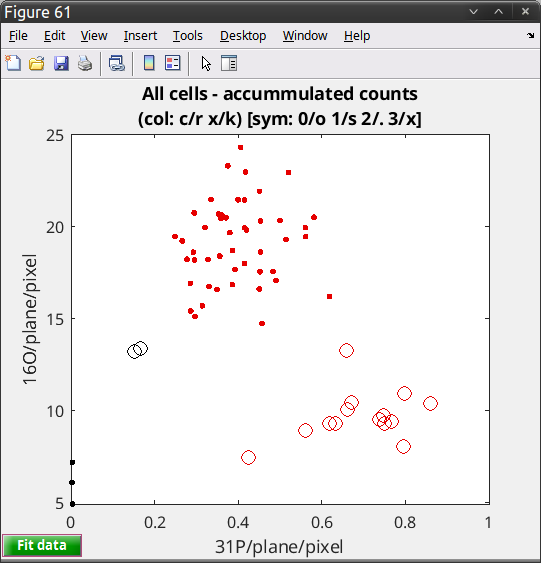
\includegraphics[width=0.34\textwidth]{figs3/LANS-metafile-scatterplot3}
\caption{\label{fig:metafile-scatterplot2}%
Example of a~scatter plot generated by metafile processing after calculating new output variables via metafile auto-processing.}
\end{figure}


\section{Less commonly used functions in LANS}
\label{sec:level3}

This section describes functions of Look@NanoSIMS that are useful under special circumstances. Many of these functions have been added based on stimulus from colleagues and collaborators, who wanted to look at their NanoSIMS data in a special way. Thus, these functions likely distinguish Look@NanoSIMS from other programs used for NanoSIMS data processing.

%\subsection{Hue intensity modulation based on rescaled ion counts}
\setcounter{step}{0}

\goldbox{}
Due to the statistical properties of the ion count data, ratio images may be noisy in areas where the ion counts of the denominator are low, possibly leading to distraction. Hue modulation intensity is designed to visually supress the noise and thus highlight the ratios in areas of interest. 
\tcbe

For example, if \ttt{12C14N} and \ttt{12C15N} ions are detected from cells deposited on a~polycarbonate filter, the ion counts will be high in areas corresponding to cells but very low in areas corresponding to the filter (Fig.~\ref{fig:hue}A--B). As a~result, the ratio image \ttt{12C15N/12C14N} will be noisy in areas on the filter, distracting the perception of the variation in the \ttt{15N/14N} ratio within cells (Fig.~\ref{fig:hue}C). 

\begin{figure}[!ht]
\centering
\begin{tabular}{ccc}
(A) & (B) & (C) \\
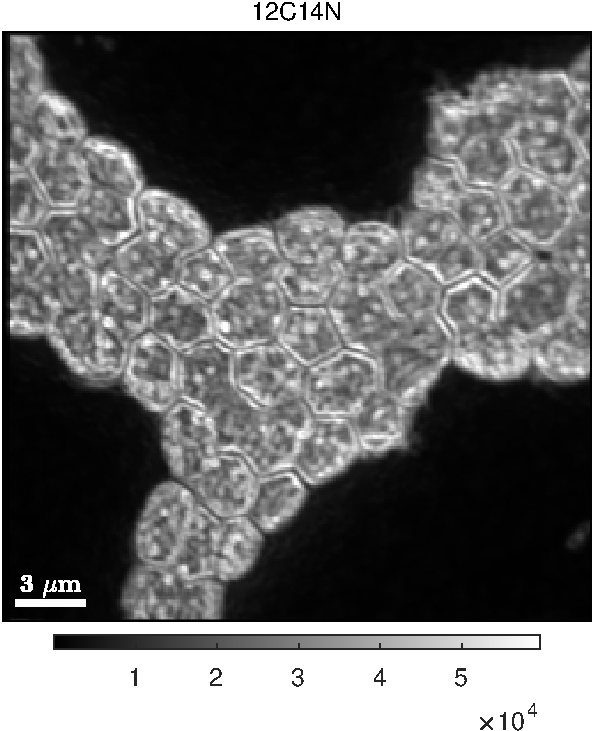
\includegraphics[scale=0.4, valign=t]{figs6/12C14N}
&
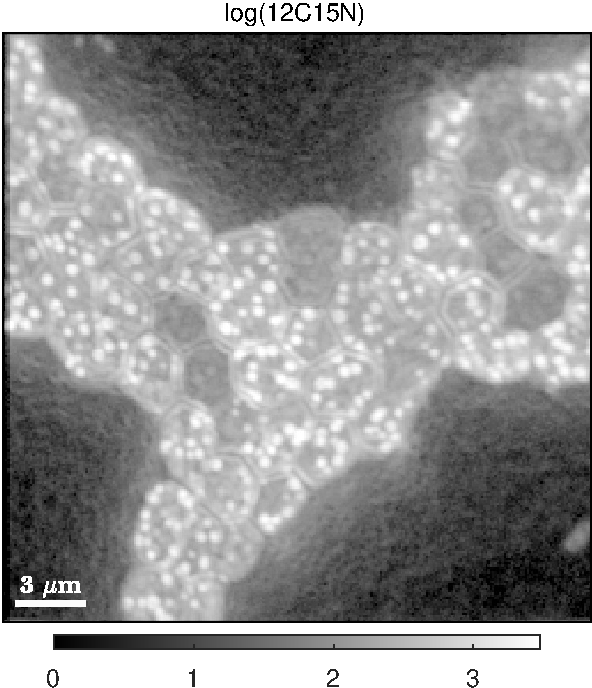
\includegraphics[scale=0.4, valign=t]{figs6/12C15N}
&
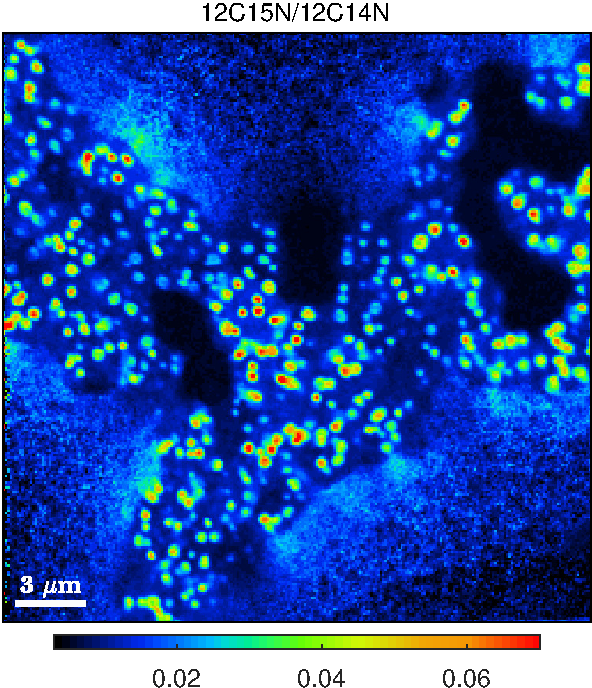
\includegraphics[scale=0.4, valign=t]{figs6/12C15N-12C14N}
\\
(D) & (E) & (F) \\
\includegraphics[scale=0.4, valign=t]{figs6/12C14Nb}
&
\includegraphics[scale=0.4, valign=t]{figs6/12C15N-12C14Nb}
&
\includegraphics[scale=0.4, valign=t]{figs6/12C15N-12C14Nc}
\end{tabular}
\caption{\label{fig:hue}%
Manipulation of the image appearance by hue intensity modulation. (A) \ttt{12C14N} ion counts, shown in the linear scale. Note the large contrast between the counts from areas with cells and areas on the filter. (B) \ttt{12C15N} ion counts, shown in the logarithmic scale. (C) \ttt{12C15N/12C14N} ratio image. Note the noise in areas on the filter. (D) The same \ttt{12C14N} ion count image as in panel~A, but rescaled such that the areas with and without cells appear white and black, respectively. (E--F) The same \ttt{12C15N/12C14N} ratio image as in panel~C, but with hue intensity modulation applied based on the image in panel~D. The areas on the filter can be shown in black (E) or white (F).}
\end{figure}

Use the following steps to manipulate the ratio image such that the noise perception from areas on the filter will be minimized, as illustrated in Fig.~\ref{fig:hue}E--F.

\s In the main LANS window, rescale the \ttt{12C14N} image (i.e., the mass that defines the cells) such that the cells will appear white and the filter will appear black (Fig.~\ref{fig:hue}D).

\s Select the \lanscb{Modulate hue intensity} checkbox and add number~4 in the \lanstf{mass} field next to it. 

\bul In this example, number 4 is chosen because for this particular dataset, the identifier of the \ttt{12C14N} mass is~4. 

\s Select \lans{Output} $\ra$ \lans{Display ratios} to re-export the \ttt{12C15N/12C14N} ratio image.

\bul The modified image will look as shown in Fig.~\ref{fig:hue}E, with areas on the filter being so dark (black) that the distracting noise is virtually invisible.

\bul You can modify this behaviour by changing the dark areas to bright (white) areas, as explained in the next steps.

\s Select \lans{Preferences} $\ra$ \lans{Additional output options}, and in the window that opens, select the \lanscb{Use white to modulate hue} checkbox and click \lans{Apply}. 

\s Then, back in the main LANS window, change the \lanstf{color} next to the \lanscb{Include ROIs outline} checkbox to \ttt{k} (corresponding to black).

\bul This will ensure that the scale bar will be visible in the exported image (i.e., displayed in black rather than white).

\s Re-export the ratio image by selecting \lans{Output} $\ra$ \lans{Display ratios}.

\bul The modified image will look as shown in Fig.~\ref{fig:hue}F, with areas on the filter being so bright (white) that the distracting noise is virtually invisible.

\vskip3mm\noindent
We emphasize that hue intensity modulation is a~powerful feature and should be used responsibly. It may be used to supress distracting but irrelevant information, such as in the example above, but \emph{not} hide distracting but possibly important information in the image.
 % done
%\subsection{Integrating an external image into the NanoSIMS dataset}
\setcounter{step}{0}

\goldbox{}
NanoSIMS measurements are compatible with correlative imaging. That is, it is possible to first measure a~sample with another imaging technique, such as TEM (transmission electron microscopy), SEM (scanning electron microscopy), or FM (fluorescence microscopy), and then image the very same area on the sample with NanoSIMS. To aid this type of correlative imaging, LANS implements functions that allow you to align an external image with the NanoSIMS image and then import the aligned external image into LANS for the purpose of defining ROIs, creating overlays, or conducting other quantitative analyses. This section explains how to do these steps in LANS.
\tcbe

As an example, we will use two input files: \ttt{Ecoli-Azo-Gam42a.im.zip} contains the NanoSIMS data (secondary ions of \ttt{12C}, \ttt{13C}, \ttt{19F}, \ttt{12C14N}, \ttt{32S} and \ttt{Esi}, Fig.~\ref{fig:LANS-ext-raw}A), while \ttt{Ecoli-Azo-Gam42a-FISH.tif} contains the FM data (green channel is the fluorescence intensity from a~microbe-specific FISH probe, blue channel is the fluorescence intensity of the DAPI stain attached to DNA of all microbes, Fig.~\ref{fig:LANS-ext-raw}B). These data are available from the same location as the LANS program (folder \ttt{data/Ecoli-Azo}).

\subsubsection{Aligning an external image with the NanoSIMS image}
\setcounter{step}{0}

\goldbox{}
Although the NanoSIMS and external images were obtained from the same area, it is very \emph{unlikely} that they look exactly the same: typically, they are distorted relative to each other by translation, rotation and heterogeneous stretching. Thus, in the first step, the external and NanoSIMS images need to be \bb{aligned}.
\tcbe

\s In the main LANS window, process the NanoSIMS dataset \ttt{Ecoli-Azo-Gam42a.im.zip} until you arrive at accumulated and scaled ion count images, as shown in Fig.~\ref{fig:LANS-ext-raw}A (see Section~\ref{sec:} for the relevant details).

\begin{figure}[!ht]
\centering
\begin{tabular}{cc}
A: \includegraphics[scale=0.665, valign=t]{figs7/Ecoli-Azo-Gam42a}
&
\raisebox{-1.6mm}{%
\begin{tabular}[t]{cc}
B: \includegraphics[scale=0.348, valign=t]{figs7/log(12C14N)-vs-log(32S)-vs-log(19F)-rgb}
\\[15mm]
C: \raisebox{-1.75mm}{\includegraphics[scale=0.2, valign=t]{figs7/Ecoli-Azo-Gam42a-FISH}}
\end{tabular}}
\end{tabular}
\caption{\label{fig:LANS-ext-raw}%
Example of (A--B) NanoSIMS and (C) fluorescence images before their integration in LANS. Panel~A shows the accumulated images of all detected ions, panel~B shows an RGB overlay of the log-transformed counts of \ttt{12C14N}, \ttt{32S} and \ttt{19F} ions. }
\end{figure}

\s Export the ion count images or RGB overlays using \lans{Output} $\ra$ \lans{Display masses}.

\nb\bul The choice depends on what you think is the best NanoSIMS image, or an RGB overlay of NanoSIMS images, based on which you will be able to align the external image.

\bul If you plan to use one of the ion count images for aligning the external image, then the relevant image data will be exported in the Matlab format (as \ttt{*.mat} files), stored in the \ttt{mat} sub-folder.

\bul In this example, choose the RGB overlay of log-transformed counts of \ttt{12C14N} (red), \ttt{32S} (green) and \ttt{19F} (blue) ions (Fig.~\ref{fig:LANS-ext-raw}B). This overlay is exported not only in PDF but also as a~\ttt{TIF} file called \ttt{log(12C14N)-vs-log(32S)-vs-log(19F)-rgb.tif}, stored in the \ttt{tif} sub-folder.

\s Select \lans{External} $\ra$ \lans{Align external and nanosims images}.

\s In the new window that opens, select \lans{File} $\ra$ \lans{Load external image}. Navigate to the file of the external image and select it.

\nb\bul In this example, select the file \ttt{Ecoli-Azo-Gam42a-FISH.tif}, which looks as shown in Fig.~\ref{fig:LANS-ext-raw}C.

\s In the same window, select \lans{File} $\ra$ \lans{Load nanosims image}. Navigate to the file you chose in step~2.

\nb\bul In this example, select the file \ttt{log(12C14N)-vs-log(32S)-vs-log(19F)-rgb.tif}.

\s Select \lans{Action} $\ra$ \lans{Add point} (\ttt{Ctrl+a}), then click within the \bb{external} image (\bb{left} panel) on a~point for which you will be able to find a~corresponding point in the NanoSIMS image (right panel).

\nb\bul After you select a point, you can use arrow keys to fine-tune its position. Press \ttt{Enter} when you are certain with the position.

\s Again, select \lans{Action} $\ra$ \lans{Add point} (\ttt{Ctrl+a}), but this time click within the \bb{NanoSIMS} image (\bb{right} panel) on a~point that correponds to the point on the external image defined in the previous step. 

\nb\bul Again, use arrow keys to fine-tune the point's position and press \ttt{Enter} to confirm it.

\s Repeat steps 6 and 7 several times to define additional points in the external image and the corresponding points in the NanoSIMS image, one pair of points at a~time.

\nb\bul The more point pairs you define, the better the alignment will be. You will need at least 4~point pairs for a~reasonably good alignment. 

\bul An example of point pairs defined in this example is shown in Fig.~\ref{fig:LANS-ext-window}.

\begin{figure}[!ht]
\centering
\includegraphics[width=0.9\textwidth]{figs7/LANS-ext-align-points}
\caption{\label{fig:LANS-ext-window}%
Example of point pairs defined in the external (left panel) and NanoSIMS (right panel) images. Points with the same identification number correspond to each other. These points are defined manually by the user based on distinct features in the images, such as cells in this example.}
\end{figure}

\bul Note that each added point will have a~unique identification number. You will be able to see which points correspond to each other in the external and NanoSIMS images based on these identification numbers.

\bul If you need to change the color of the point or an identifier, you can do this by selecting \lans{Action} $\ra$ \lans{Change point's color}.

\s If you need to modify a~point's location, select \lans{Action} $\ra$ \lans{Modify point}, then click on the point you want to modify and press \ttt{Enter} to confirm the selection. Subsequently, use arrow keys to modify the point's location, and finally press \ttt{Enter} to confirm thew new location.

\nb\bul Observe messages in the Matlab console for more details about what exactly you need to do.

\s If you need to remove a~pair of corresponding points, select \lans{Action} $\ra$ \lans{Remove pair of points}, then click on one of the points in the pair and press \ttt{Enter} to confirm the removal.

 \s After defining a reasonably high number of point pairs (typically 5--10 should be sufficient), select \lans{File} $\ra$ \lans{Save point list} to save the points' coordinates in a~matlab file. 
 
 \nb\bul You can load these coordinates later via \lans{File} $\ra$ \lans{Load point list}. Subsequently, you can add more points, modify points, or remove points, as described in steps 6--10.

\s If the selected NanoSIMS image does not contain all features based on which you can align the external image, you can load a~\bb{different} NanoSIMS image at any time (see step~5). When doing so, you may need to select \lans{Action} $\ra$ \lans{Update points} to redraw the currently defined points in the image.

\s Select \lans{Action} $\ra$ \lans{Alignment based on N$>$4 points} to \bb{perform the image alignment} based on the defined point pairs.

\nb\bul
The result will be displayed in a~new window (Fig.~\ref{fig:LANS-ext-result}). You can quality-check the alignment by changing the transparency of the layers displaying the external and NanoSIMS images through the \lans{Transparency} menu or, more quickly, by pressing \ttt{Ctrl+1} -- \ttt{Ctrl+4} keys.

\begin{figure}[!ht]
\centering
\begin{tabular}{ccc}
A & B & C \\
\includegraphics[scale=0.23]{figs7/LANS-ext-result1}
&
\includegraphics[scale=0.23]{figs7/LANS-ext-result2}
&
\includegraphics[scale=0.23]{figs7/LANS-ext-result3}
\end{tabular}
\caption{\label{fig:LANS-ext-result}%
Results of the image alignment are shown as an overlay. Panels (A--C) show the overlays at different levels of transparency of the external and nanoSIMS image layers. These levels can be changed through the \lans{Transparency} menu. Note the match between the point pairs defined in the external ($\times$) and nanoSIMS ($+$) images. Although the external image was originally an RGB image in this example, the image is converted to a~grayscale in the overlay.}
\end{figure}

\s If you are satisfied with the result, select \lans{Action} $\ra$ \lans{Export aligned external image} to \bb{store the aligned external image} for later use. If not, repeat steps~6--13.

\nb\bul Specify an appropriate name (e.g., \ttt{ext\_aligned}) and location of the file. You can store it in a~Matlab (\ttt{*.mat}) or TIF (\ttt{*.tif}) format. It is a~good idea to store them in both formats and in the folder with all the other processed data.

%%%

\subsubsection{Importing an aligned external image}
\setcounter{step}{0}

\goldbox{}
Once the external image is aligned with the NanoSIMS images, it can be imported into LANS using the following steps.
\tcbe

\s In the main LANS window, select \lans{External} $\ra$ \lans{Select aligned external image}, navigate to the image, and click \lans{Open} to select it. 

\nb\bul If the external image is an~RGB image, as in this example, you will be asked to select \bb{one} channel (\ttt{r}, \ttt{g}, or \ttt{b}) to fully define the external image. This is because currently LANS only supports a~single-channel (i.e., grascale) external images. In this example, choose channel \lanstf{g} to load the channel corresponding to the fluorescence from the microbe-specific FISH probe.

\s Read carefully the note that appears after you load the image. It tells you that the external image has been \bb{integrated} into the NanoSIMS dataset and can be used as a~\bb{regular mass} with the name \lanstf{ext}.

%%%%

\subsubsection{Using the external image with the NanoSIMS images}
\setcounter{step}{0}

\goldbox{}
After importing the aligned external image into LANS, the image can be used, effectively, as if it were one of the masses in the NanoSIMS dataset. By default, the name of this `extra mass' is \lanstf{ext}. This name can then be used, for instance, as a~template for ROI definition or to create overlays with NanoSIMS images or scatter plots, as described in the following example.
\tcbe

\s Type \ttt{ext} into one of the ratio \lanstf{expression} text fields, specify the \lanstf{scale} (e.g., you can start with \ttt{[0 1]}), and press \ttt{Enter} to display the scaled external image.

\nb\bul This will reassure you that the external image is really usable as part of the NanoSIMS dataset.

\s To use the external image for defining ROIs, type \ttt{ext} in the \lanstf{ROI definition template} and proceed as described in Section~\ref{sec:} to define ROIs.

\nb\bul This is an example where \lans{Interactive thresholding} will really speed up the  ROI definition.

\bul After using the green channel of the external image as a~template, the ROIs may look as shown in Fig.~\ref{fig:LANS-ext-ROIs}A.

\def\scf{0.22}
\begin{figure}[!ht]
\centering
\begin{tabular}{ccc}
A & B & C \\
\includegraphics[scale=\scf]{figs7/LANS-ext-ROIs1}
&
\includegraphics[scale=\scf]{figs7/LANS-ext-ROIs2}
&
\includegraphics[scale=\scf]{figs7/LANS-ext-ROIs3}
\end{tabular}
\caption{\label{fig:LANS-ext-ROIs}%
ROI definition using an aligned external image. (A) First set of ROIs defined based on the green channel of the external image. (B) Added and revised ROIs defined based on the blue channel of the external image. (C) Final set of ROIs.}
\end{figure}

\goldbox{}
This step is specific to this particular example, but it gives you an idea about the \emph{iterative} process of using an external image during NanoSIMS data processing. 
\tcbe

\s Based on the original external image, it is clear that not all cells are visible in the green channel. To define all cells in the image, the blue channel needs to be used instead. Thus, import the external image again as described in the previous section, but this time choose channel \lanstf{b} (DAPI flurescence) instead of \lanstf{g}. Then proceed with step~2 to continue ROI definition.

\nb\bul After using the blue channel of the external image as a~template, the revised ROIs may look as shown in Fig.~\ref{fig:LANS-ext-ROIs}B.

\s Classify the ROIs using steps described in Section~\ref{sec:}.

\nb\bul
You can base this classification on the aligned external image, where you clearly see (in most cases) the differences between cells only stained with DAPI (blue) and cells stained with both DAPI and the FISH probe (cyan). You can use, for instance, \ttt{b} and \ttt{c} as the class names for the respective cells.

\s Type \ttt{ext/pixel} into one of the ratio \lanstf{expression} text fields and specify the \lanstf{scale}.

\nb\bul This is necessary if you want to properly normalize the ROI-specific values for the external image data.

\s Create overlays between the external image and one of the NanoSIMS images, or scatter plots between the ROI-specific values in the external and NanoSIMS images, using steps described in Section~\ref{sec:}. 

\nb\bul Examples of the results may look as shown in Fig.~\ref{fig:LANS-ext-overlays}.

\def\scf{0.42}
\begin{figure}[!ht]
\centering
\begin{tabular}{cc}
A: \includegraphics[scale=\scf, valign=t]{figs7/19F-plane-pixel-vs-ext-pixel-vs-ext-pixel-rgb}
&
B: \includegraphics[scale=\scf, valign=t]{figs7/19F-plane-pixel-vs-ext-pixel}
\\
{ } & { } \\
C: \includegraphics[scale=\scf, valign=t]{figs7/13C-(12C+13C)-vs-ext-pixel-rgb}
&
D: \includegraphics[scale=\scf, valign=t]{figs7/13C-(12C+13C)-vs-ext-pixel}
\end{tabular}
\caption{\label{fig:LANS-ext-overlays}%
Examples of results combining ROI-specific values derived from the external and NanoSIMS images. They show that in most cells, there is a~clear correspondence between the ROI-specific intensity of the \ttt{19F} ion counts and the FISH signal (panels A--B). They also show that most of the FISH-stained cells are highly enriched in the ${}^{13}C$ isotope and vice versa (C--D). Cells for which these statements are not valid require closer inspection.}
\end{figure}

\s When you are finished using the external image, it is a~good idea to \bb{remove} it from the NanoSIMS dataset. You can do this by selecting \lans{External} $\ra$ \lans{Select aligned external image} and clicking \lans{Cancel}. Also, do not forget to store preferences at the end of your analysis.

%%%%

\subsubsection{Resampling of NanoSIMS images to match resolution of an external image}
\setcounter{step}{0}

\goldbox{}
In addition to rotation, stretching or other types of image distortion, it can happen that the external and NanoSIMS images have a~very different pixel resolution. For example, in the example below, the TEM image has roughly 10-fold higher resolution than the NanoSIMS image. If you want to use such a~high-resolution TEM image as a~template for defining ROIs, which can then be used to quantify ROI-specific NanoSIMS data such as ion counts or ratios, it is necessary to rescale the NanoSIMS images to match the resolution of the external image. This can be done by resampling the NanoSIMS images, as described in the following steps.
\tcbe

\nb Work in progress.

	% mostly done, except for resampling of ext
%\subsection{Depth variation of isotope ratios --- basic visualization}
\setcounter{step}{0}

\goldbox{}
\begin{minipage}[c]{0.5\textwidth}
During a~NanoSIMS measurement, the sample material is gradually \bb{eroded} by the primary ion beam while the emitted secondary ions are sepa\-rated based on their mass and detected. The ion counts in the subsequent planes therefore record a~\bb{depth} variation of the elements and isotopes within the sample, making it possible to reconstruct their distribution in~3D. This section describes how to use LANS to visualize this 3D variation in the most basic way: by displaying \bb{lateral profiles along depth} in the sample.
\end{minipage}\hfill
\begin{minipage}[c]{0.48\textwidth}
\includegraphics[width=3.5cm, valign=c]{figs3/18O-(16O+18O)-ilp.png}
$\rightarrow$
\includegraphics[width=3.5cm, valign=c]{figs3/18O-(16O+18O)-lpd.png}
\end{minipage}

\tcbe

To obtain a~good quality dataset for 3D reconstruction, the measurement needs to use a~relatively low primary ion current to achieve sufficient lateral resolution. At the same time, the same field of view on the sample needs to be measured repeatedly in \bb{many planes} to erode the sample along a~substantial depth interval (several microns) such that a~meaningful 3D variation in this interval occurs. The number of detected planes can start from several hundreds, but it can reach up to several thousands (the example below will use 7000 planes). However, one NanoSIMS measurement in the imaging mode is limited to a~maximum of 1000~planes, which means that the analysis of the same sample area needs to be done as a~\bb{chain} of multiple imaging analyses. This measurement approach leads to multiple raw datasets, which need to be \bb{merged} and analyzed as \bb{one} dataset. Thus, one of the challenges of isotope ratio visualization along depth is the need to load multiple raw datasets and merging them into a~single stack with potentially several thousands of images. 

Another important challenge stems from the fact that because ion count rates for minor isotopes (e.g., ${}^{13}\mathrm{C}$) are typically very low, ion count ratios derived from those minor isotopes (e.g., \ttt{13C/12C}) will generally be noisy if based on data in a~single plane. To maximize the signal-to-noise ratio in depth profiles of isotope ratios while maintaining an acceptable depth resolution, it is better to handle the original ion count data in \bb{blocs} of multiple subsequent planes, where the counts in each bloc are summed up (across the planes but separately for each pixel in the lateral dimension) and treated as \bb{one} plane.  

Overall, basic visualization of the 3D variation in isotope ratios involves three major steps: (i) loading the raw dataset in blocs, possibly involving loading and merging of multiple datasets, (ii) drift-correcting the planes within each bloc before they are summed up into a~single plane, and finally (iii) visualization of lateral profiles along depth. This section describes how to do these processing steps in LANS. 

The example uses data acquired in collaboration with Nicole Geerlings and Filip Meysman, as documented in the following open-access publications:
\vskip1mm
\begin{center}
\begin{minipage}{0.93\textwidth}
\textsl{\small Geerlings et al.~(2021) Cell Cycle, Filament Growth and Synchronized Cell Division in Multicellular Cable Bacteria. \emph{Front Microbiol}~\bb{12}:620807}. \url{https://doi.org/10.3389/fmicb.2021.620807}
\vskip1mm
\textsl{\small Geerlings et al.~(2022) Polyphosphate Dynamics in Cable Bacteria. \emph{Front Microbiol}~\bb{13}:883807}. \url{https://doi.org/10.3389/fmicb.2022.883807}
\end{minipage}
\end{center}
\vskip1mm
The data is available in the same location as the LANS program (folder \ttt{test\_data/NS+3D}) and includes 7~datasets (\ttt{2020-03-26-ELFIL\_2.im.zip} \dots\ \ttt{2020-03-26-ELFIL\_8.im.zip}) acquired in a~chain of 7~consecutive scans of cable bacteria placed on a~polycarbonate membrane filter. Each dataset comprizes 1000~planes. The first dataset (\ttt{ELFIL\_2}) was acquired using dwell time of 1000\,ms, whereas the remaining datasets used the dwell time of 2000\,ms.

\subsubsection{Loading datasets in blocs, merging multiple datasets}
\setcounter{step}{0}

\s{In preparation for the subsequent steps, first select \lans{Input} $\ra$ \lans{Load raw dataset} to load \bb{all} planes in the first dataset (\ttt{2020-03-26-ELFIL\_2.im.zip}).}

\nb{This step is required to determine the \lanstf{base mass for alignment} and \lanstf{special region for alignment}, which are necessary later for automatically drift-correcting planes in a~bloc.}

\s{Proceed as described in Sections \ref{sec:display-masses-plane-by-plane} (steps 1--3) and \ref{sec:drift-correction-accumulation} (steps 1--2) to define the \lanstf{base mass for} \lanstf{alignment} and \lanstf{special region for alignment}.}

\nb{At this stage, you should \emph{not} proceed with image accumulation (steps 3--4 in Section~\ref{sec:drift-correction-accumulation}) just yet, because the planes need to be first drift-corrected and accumulated \emph{within} blocs. Instead, proceed as described in the following.}

\s{Select \lans{Input} $\ra$ \lans{Load multiple RAW datasets in blocs}. }

\sbx{Navigate to the raw files and select them, using the \ttt{Ctrl} key to select multiple files.}

\nbx{When choosing the analysis of data in blocs, you do \emph{not} necessarily need to load multiple datasets. Indeed, you can choose one dataset if you only want to perform the analysis in blocs just for that one dataset. If you do load multiple datasets, however, such as in this example, make sure that they have all been acquired with the same pixel resolution (e.g., $256\times 256$ pixels).}

\s{In the dialog window that opens, specify the \lanstf{bloc size}, i.e., the number of planes per bloc. If you are going to load data from multiple datasets, indicate whether or not you want to use the same bloc size for all subsequent datasets.}

\nbx{In this example, you will use the bloc size of 100 for the first dataset (\ttt{2020-03-26-ELFIL\_2.im.zip}) and 50 for the other six datasets. This is because the dwell time used to acquire the first dataset was $2\times$ shorter (1\,ms) than the dwell time used for the other datasets (2\,ms). Thus, in the dialog window, first enter 100 in the first field (bloc size) and 0 (\ttt{=no}) in the second field. Then, when loading the subsequent datasets, enter 50 in the first field (bloc size) and 1 (\ttt{=yes}) in the second field.}

\s{Click \lans{OK} in the dialog window and observe the progress of loading in the Matlab console.}

\nbx{First, the raw data will be loaded. Then, the drift-correction information for planes in each bloc will be calculated based on the values for \lanstf{Base mass for alignment} and \lanstf{Special region} \lanstf{for alignment} (see Step~2 above). Subsequently, this information will be applied to drift-correct and accumulate planes in blocs for each mass.}

\nnb{If you selected multiple raw datasets, the same steps will be repeated for each of them.}

\nnb{After this step is completed, the dataset loaded in LANS will ``behave'' as any other raw dataset loaded via \lans{Input} $\ra$ \lans{Load RAW dataset}. The only difference will be that each individual plane is, in fact, a~sum of multiple planes (i.e., an accumulated bloc of planes). Thus, the subsequent analysis will proceed according to the same steps as for any other dataset. }

\s{In particular, you need to start with the drift-correction and accumulation of planes via \lans{Input} $\ra$ \lans{Accumulate plane images} (Section~\ref{sec:drift-correction-accumulation}, steps 3--4).}

\nbx{This is because although the individual planes were drift-corrected \emph{within} each bloc (during the loading process), the drift-correction also needs to be calculated and applied \emph{between} blocs.}

\s{Select \lans{Output} $\ra$ \lans{Save FULL PROCESSED data} to save the image stack, for all masses and all planes, in a~Matlab format (extension \ttt{mat}).}

\nbx{This is highly recommended because the loading of data in blocs, accompanied with drift-correction and accumulation, is quite laborious and may be time consuming. Thus, you likely do not want to do it again for the very same dataset or group of datasets. }

\nnb{When saving the data, use the default filename suggested by LANS, unless you really want to use a~different one. Note that the default filename will end with \ttt{bN.mat}, where \ttt{b} refers to the fact that the data was loaded in blocs and \ttt{N} corresponds to the number of planes per bloc (bloc size). In this example, choose the default filename \ttt{2020-03-26-ELFIL\_b100.mat}.}

\nnb{Beware that if the final dataset contains many planes, the exported \ttt{mat} file may be quite large (e.g., hundreds of Mb). Still, this is an acceptable price to pay for not having to load the same multiple datasets in blocs again.}

%%

\subsubsection{Visualization of lateral profiles along depth in the sample}
\setcounter{step}{0}

\goldbox{}
Although you can perform this analysis with any NanoSIMS dataset, it is most useful for datasets that have been loaded in blocs, as described in the previous section.
\tcbe

\s{In the main LANS window, select the \lanscb{Display lateral profiles} checkbox in the \ttt{Output options} box.}

\nbx{If you only want to focus on the analysis of lateral profiles, it is a~good idea if you deselect other checkboxes in the \ttt{Output options} box (except for the \lanscb{Export ASCII data} and \lanscb{Export PDF graphics} checkboxes, which should remain selected).}

\s{In the \lanstf{expression} and \lanstf{scale} fields, specify the formulas for the ion count ratios you want to analyze and the corresponding scale. }

\nbx{In this example, you will look at depth profiles of ${}^{13}C/({}^{12}C+{}^{13}C)$, ${}^{18}O/({}^{16}O+{}^{18}O)$, $O/plane/pixel$ and $P/plane/pixel$. Thus, enter \ttt{13C14N/(12C14N+13C14N)}, \ttt{18O/(16O+18O)}, \ttt{16O/plane/pixel} and \ttt{31P/plane/pixel} in the expression fields. Then experiment with the optimal scales.}

\nnb{Do not forget to check the corresponding checkboxes next to the formulas.}

\s{Select \lans{Output} $\ra$ \lans{Display ratios}. }

\sbx{In the top-left corner of the new window that opens (Fig.~\ref{fig:lateral}A), select the variable based on which you want to define (draw) a~lateral profile.}

\begin{figure}[!ht]
\centering
\begin{tabular}{cc}
A: \includegraphics[scale=0.3, valign=t]{figs3/LANS-lateral1}
&
B: \includegraphics[scale=0.3, valign=t]{figs3/LANS-lateral2}
\end{tabular}
\caption{\label{fig:lateral}%
(A) LANS window for the analysis of variation in ion counts and ion count ratios along a~\bb{lateral} profile. If the \lanscb{Show depth variation} checkbox is selected (marked in blue), the variation along \bb{depth} will also be displayed. Such variations are displayed for all variables selected in the listbox below the checkbox (marked in yellow). The thickness of the lateral profile (red mark) and the color-scale of each variable (brown marks) can also be adjusted. (B) Results of this particular analysis show, among other things, that (i) in the ${}^{13}\mathrm{C}$ non-enriched cells, polyphosphate inclusions, identified as round (oval) areas with markedly higher signals of $P$ and $O$, are significantly and roughly homogeneously enriched in ${}^{18}\mathrm{O}$ relative to the rest of the cell biomass, whereas (ii) the cells enriched in ${}^{13}\mathrm{C}$ show ${}^{18}\mathrm{O}$ enrichment in the polyphospate inclusions as well as in the cytoplasm and DNA.}
\end{figure}

\nbx{In this example, you will look at depth variation in the ${}^{18}O/({}^{16}O+{}^{18}O)$ ratio in polyphosphate inclusions. Thus, select \ttt{18O/(16O+18O)}.}

\s{Click on \lans{Draw polyline} to draw a~lateral profile in the image.}

\nbx{The profile can have multiple vertices (hence the name `polyline'), allowing you to create profiles along a~``curved'' profile or even make sharp corners (Fig.~\ref{fig:lateral}A).}

\nnb{Double-click to define the last vertex of the polyline. Although this will stop the polyline drawing mode, you can still continue adding, moving or removing vertices after this point by clicking with the right mouse button on the polyline. You can also move the entire polyline or remove it and start over.}

\s{Specify the \lanstf{Profile thickness}, in pixels.}

\nbx{For the default value of 1, the lateral profile will be based on values in \bb{one} pixel nearest to the polyline. Because this may yield a~rather noisy output, it is recommended to use a~greater value here. For example, using the profile thickness of~5, the lateral profile will be based on values in 5~pixels nearest to the polyline (2~on one side, 2~on the other side, 1~on the polyline). Thus, you can think of the profile as being based on data in a~`band' along the polyline.}

\s{Select the \lanscb{Show depth variation} checkbox (highlighted in blue in Fig.~\ref{fig:lateral}A).}

\sbx{In the list of variables (highlighted in yellow in Fig.~\ref{fig:lateral}A), select variables that you want to analyze simultaneously.}

\nbx{Hold \ttt{Ctrl} to select multiple variables. In this example, select all variables.}

\s{Click on \lans{Display lateral profiles}.}

\nbx{This will open a new window showing the variation of the selected variables along the lateral profile (`band') and depth (Fig.~\ref{fig:lateral}B).}

\s{Select the \lanscb{Export} checkboxes and click again on \lans{Display lateral profiles} to export the results as ASCII text and PDF images.}

\s{Click on \lans{Save polyline} to save the polyline coordinates.}

\nb{You can load it in the future by clicking on \lans{Load polyline}.}
 % done, results need to be updated
\subsection{Loading datasets with more than 8 masses}
\setcounter{step}{0}

\goldbox{}
During a~typical NanoSIMS measurement, at most 8~different ionic species are recorded: 7~different isotopes, and secondary electrons (normally denoted as \ttt{Esi}). This explains the visual design of LANS, which contains 8~fields for \lanstf{detected masses}. However, NanoSIMS instrument can operate in a~so-called peak-switching mode, which allows quasi-simultaneous detection of up to 15~different ionic species ($2\times 7$ different isotopes and \ttt{Esi}). This section explains how to use LANS to analyze datasets containing counts of more than 8~ionic species.
\tcbe

\noindent
This feature was added to LANS based on a~request from Dr.~Hryhoriy Stryhanyuk (UFZ Leipzig). In the example below, we use one of the datasets acquired in his lab to illustrate the approach: \ttt{2022-01-25-OPG\_1.im.zip}.

\vskip0.5\baselineskip

\sbx{Load the raw dataset.}

\nbx{This is done in the usual way, as for any other dataset. Based on the structure of the data within the binary file, LANS will automatically recognize that it was acquired in a~peak-switching mode and rearrange the data accordingly.} 

\nnb{%
An example of the output generated during loading is shown here:
\begin{center}
\includegraphics[scale=0.34]{figs8/LANS-8plus-load}
\end{center}
}

\s{After loading, it is a~good idea to first find out which ions were actually detected. This is best done by selecting \lans{Input} $\ra$ \lans{Autoscale plane images}.}

\nnb{In this example, LANS indicated that data from 16 masses were detected (see output above). However, some of the masses were recorded repeatedly because not all detectors used peak-switching during ion detection. In fact, the number of \emph{different} ionic species detected in this example was~12: ${}^{16}\mathrm{O}{}^1\mathrm{H}$, ${}^{16}\mathrm{O}{}^2\mathrm{H}$, ${}^{12}\mathrm{C}_2$, ${}^{12}\mathrm{C}{}^{13}\mathrm{C}$, ${}^{12}\mathrm{C}{}^{14}\mathrm{N}$, secondary electrons (\ttt{Esi}), ${}^{12}\mathrm{C}{}^{15}\mathrm{N}$, ${}^{32}\mathrm{S}$, ${}^{12}\mathrm{C}_2{}^{1}\mathrm{H}$, ${}^{12}\mathrm{C}_2{}^{2}\mathrm{H}$, ${}^{13}\mathrm{C}{}^{14}\mathrm{N}$, and ${}^{31}\mathrm{P}{}^{1}\mathrm{H}$, as follows from the output in the Matlab console:
\begin{center}
\includegraphics[scale=0.34]{figs8/LANS-8plus-autoscale}
\end{center}}

\nb{It is important the realize that due to the limited number of fields dedicated to detected \lanstf{masses} in the LANS user interface (maximum~8), all of these ionic species \emph{cannot} be displayed in the list. Indeed, only the first 8~masses are included in the list. Nevertheless, they \emph{are} registered internally within the list of detected masses and can therefore be used in any of the \lanstf{expressions} (see below).}

\sbx{Select \lans{Input} $\ra$ \lans{Display plane images for all masses} to view the raw ion counts, plane by plane.}

\nnb{Note that some masses only show non-zero counts in \emph{every second plane}. This is because the specific detectors used peak switching to alternately detect two ionic species at the same nominal mass. In this example, it concerns the following pairs: ${}^{12}\mathrm{C}{}^{13}\mathrm{C}$ \& ${}^{12}\mathrm{C}_2{}^{1}\mathrm{H}$ at nominal mass~25, ${}^{12}\mathrm{C}{}^{14}\mathrm{N}$ \& ${}^{12}\mathrm{C}_2{}^{2}\mathrm{H}$ at nominal mass~26, ${}^{12}\mathrm{C}{}^{15}\mathrm{N}$ \& ${}^{13}\mathrm{C}{}^{14}\mathrm{N}$ at nominal mass~27, and ${}^{32}\mathrm{S}$ \& ${}^{31}\mathrm{P}{}^{1}\mathrm{H}$ at nominal mass~32 (Fig.~\ref{fig:LANS-8plus-frames}A--B).}

\begin{figure}[!ht]
\centering
\begin{tabular}{c}
A: \includegraphics[scale=0.43, valign=t]{figs8/m-001}
\\
B: \includegraphics[scale=0.43, valign=t]{figs8/m-002}
\\
C: \includegraphics[width=0.86\textwidth, valign=t]{figs8/2022-01-25-OPG-all}
\end{tabular}
\caption{\label{fig:LANS-8plus-frames}%
Example of raw data acquired via peak-switching mode. Panels (A--B) show ion counts in the first two planes, as obtained by selecting \lans{Input} $\ra$ \lans{Display plane images for all masses}. Note that only the first 8~masses are displayed in this way, although a~total of 12~different masses were detected. This is due to the limitation of the  graphical interface of LANS. This limitation, however, does not impede further analysis of the data by LANS. Panel C shows the accumulated ion count images, as obtained by selecting  \lans{Input} $\ra$ \lans{Display accumulated images for all masses}. In this case, all 12~detected masses are displayed side-by-side.}
\end{figure}

\s {While viewing the detected ions in the previous step, identify suitable mass that can be used as a~\lanstf{Base mass for alignment} and type it into the corresponding text field.}

\nbx{Clearly, this mass should have non-zero ion counts in \emph{every} plane to yield valid drift correction information.}

\nnb{In this example, it cannot be \ttt{12C14N}. Instead, \ttt{Esi} is a good candidate, as it is detected in every plane and has sufficiently high counts and contrast in individual planes. \ttt{12C2} could be another good candidate. }

\sbx{Select \lans{Input} $\ra$ \lans{Accumulate plane images} to accumulate drift-corrected ion images.}

\nnb{As usual, the \lanscb{Align images when accumulating} checkbox needs to be checked if you want to perform drift correction during accumulation of planes.}

\s{Select \lans{Input} $\ra$ \lans{Autoscale accumulated images} and then  \lans{Input} $\ra$ \lans{Displayed accumulated images} \lans{for all masses} to autoscale and display accumulated images for all masses.} 

\nnb{In contrast to the display of individual planes, this will visualize accumulated images for \emph{all} detected masses, providing a~full view of the raw data (Fig.~\ref{fig:LANS-8plus-frames}C).}
 
\sbx{Proceed as described in Section~\ref{sec:level1} to analyze ion counts, ion count ratios, or conduct other types of analysis.}

\nnb{Examples of the output generated for this type of data are shown in Fig.~\ref{fig:LANS-8plus-ratios}.}

\nbx{When analyzing data with more than 8~masses, you need to pay special attention to the following: If you want to display (and export) ion count images for masses that are \emph{not} displayed in the list of 8~detected masses, you need to type the name of the mass in the \lanstf{expression} field for the \bb{ratio}, as illustrated in Fig.~\ref{fig:LANS-8plus-extra-masses}, adjust the scale, and then select \lans{Output} $\ra$ \lans{Display ratios}. For example, you need to proceed in this way to display images of ${}^{12}\mathrm{C}_2{}^{1}\mathrm{H}$ (\ttt{12C21H}), ${}^{12}\mathrm{C}_2{}^{2}\mathrm{H}$ (\ttt{12C22H}), ${}^{13}\mathrm{C}{}^{14}\mathrm{N}$ (\ttt{13C14N}), or ${}^{31}\mathrm{P}{}^{1}\mathrm{H}$ (\ttt{31P1H}).}

\nb{Additionally, you need to pay extra attention when defining \lanstf{expressions} for isotope ratios. For example, if the molecular ions of ${}^{12}\mathrm{C}{}^{13}\mathrm{C}$ and ${}^{12}\mathrm{C}_2$ were detected in every plane, the correct expression for obtaining the atomic ${}^{13}\mathrm{C}/{}^{12}\mathrm{C}$ isotope ratio would be \ttt{0.5*12C13C/12C2}. However, because in this example the molecular ions of ${}^{12}\mathrm{C}{}^{13}\mathrm{C}$ were only detected in every second plane, while the molecular ions of ${}^{12}\mathrm{C}_2$ were detected in every plane, the correct expression for the ${}^{13}\mathrm{C}/{}^{12}\mathrm{C}$ isotope ratio is \ttt{12C13C/12C2}.}

\sbx{When finishing the analysis, don't forget to save the preferences by selecting \lans{Preferences} $\ra$ \lans{Store preferences}.}

\def\scf{0.36}
\begin{figure}[!h]
\centering
\begin{tabular}{ccc}
A & B & C \\
\includegraphics[scale=\scf, valign=t]{figs8/12C13C-12C2}
&
\includegraphics[scale=\scf, valign=t]{figs8/13C14N-12C14N}
&
\includegraphics[scale=\scf, valign=t]{figs8/12C15N-12C14N}
\\
D & E & F\\
\includegraphics[scale=\scf, valign=t]{figs8/16O2H-16O1H}
&
\includegraphics[scale=\scf, valign=t]{figs8/12C22H-12C21H}
&
\includegraphics[scale=\scf, valign=t]{figs8/12C15N-12C14N-vs-12C22H-12C21H-vs-12C13C-12C2-rgb}
\end{tabular}
\caption{\label{fig:LANS-8plus-ratios}%
Examples of isotope ratio images derived from data collected via peak-switching mode, illustrating the power of this measurement approach for multi-isotope imaging mass spectrometry. Panels (A--B) show the ${}^{13}\mathrm{C}/{}^{12}\mathrm{C}$ isotope ratio obtained from two different ion pairs: ${}^{12}\mathrm{C}{}^{13}\mathrm{C}$ \&\ ${}^{12}\mathrm{C}_2$ and ${}^{13}\mathrm{C}{}^{14}\mathrm{N}$ \&\ ${}^{12}\mathrm{C}{}^{14}\mathrm{N}$. Panel C shows the ${}^{15}\mathrm{N}/{}^{14}\mathrm{N}$ isotope ratio obtained from the ion pair ${}^{12}\mathrm{C}{}^{15}\mathrm{N}$ \&\ ${}^{12}\mathrm{C}{}^{14}\mathrm{N}$. Panels (D--E) show the ${}^{2}\mathrm{H}/{}^{1}\mathrm{H}$ isotope ratio obtained from two different ion pairs: ${}^{16}\mathrm{O}{}^{2}\mathrm{H}$ \&\ ${}^{16}\mathrm{O}{}^{1}\mathrm{H}$ and ${}^{12}\mathrm{C}_2{}^{2}\mathrm{H}$ \&\ ${}^{12}\mathrm{C}_2{}^{1}\mathrm{H}$. Panel F shows an RGB overlay between the three isotope ratios: ${}^{15}\mathrm{N}/{}^{14}\mathrm{N}$ (red), ${}^{2}\mathrm{H}/{}^{1}\mathrm{H}$ (green), and ${}^{13}\mathrm{C}/{}^{12}\mathrm{C}$ (blue).}
\end{figure}

\begin{figure}[!hb]
\centering
\includegraphics[scale=0.42, valign=t]{figs8/LANS-8plus-masses-ratios}
\caption{\label{fig:LANS-8plus-extra-masses}%
Processing of data acquired using peak-switching mode. Text fields on the left only contain the first 8~masses present in the dataset (marked by green). If you want to display the other masses in the dataset, you need to type their name in one of the \lanstf{expression} text fields on the right (marked by red), adjust the scale, and then select \lans{Output} $\ra$ \lans{Display ratios}. Similarly, you can use the names in \lanstf{expressions} to calculate ion count ratios (marked by blue).}
\end{figure}


%\subsection{Exporting graphics as PNG}
\setcounter{step}{0}

\goldbox{}
By default, graphical output generated by LANS is exported in the PDF format, with files stored in the \ttt{pdf} sub-folder. This output is of publishing quality. Sometimes, however, you may want to export the graphics as bitmaps in the PNG format. One of the reasons for doing this may be that the PNG files are usually smaller than the PDF files and are therefore more convenient to include in presentations. Use the following steps to export the graphics as PNG files.
\tcbe

\s{In the main LANS window, select \lans{Preferences} $\ra$ \lans{Additional output options}.}

\s{In the new window that opens, select the \lanscb{PNG} checkbox in the the \ttt{Export graphics} box and click \lans{Apply}.}

\s{In the main LANS window, export the mass or ratio images by selecting \lans{Output} $\ra$ \lans{Display masses} or \lans{Display ratios}.}

\nbx{The PNG output will be stored in the \ttt{png} sub-folder. It will look very similar to the PDF output, but it will be  a~bitmap with a~limited resolution rather than vector graphics.}

\s{Uncheck the \lanscb{PNG} checkbox if you no longer want to export the output as PNG. This will save some disk space.}

%\subsection{Exporting graphics as TIF}
\setcounter{step}{0}

\goldbox{}
Sometimes, you may want to export the nanoSIMS image data as TIF images. Such images can be used, for example, for quantitative image analysis by other, third-party software.  Use the following steps to export the images of ion counts and ion count ratios as TIF files. 
\tcbe

\s{In the main LANS window, select \lans{Preferences} $\ra$ \lans{Additional output options}.}

\s{In the new window that opens, select the \lanscb{TIFF (if BW)} checkbox in the the \ttt{Export graphics} box and click \lans{Apply}.}

\s{Back in the main LANS window, select the \lanscb{B/W} checkbox next to the \lanstf{scale} of the mass or ratio image that you want to export as TIF, then select \lans{Output} $\ra$ \lans{Display masses} or \lans{Display ratios} to export the mass or ratio images.}

\nbx{The image data will be exported as a~16-bit grayscale TIF image, stored in the \ttt{tif} sub-folder. }

\nnb{The dynamic range of the grayscale values in the exported TIF image will correspond to the image \lanstf{scale} set in the main LANS window. For example, if a~\ttt{12C} ion count image is displayed in the scale \ttt{[min max] = [20 25000]}, the grayscale values in the image pixels varying between fully black (intensity 0) and fully white (intensity $2^{16}-1=65535$) will correspond linearly to the dynamic range of the ion counts between 20 and 25000. Similar linear relationship between the image scale and the grayscale values of the exported TIF holds for the ion count ratio images.}

\s{Uncheck the \lanscb{TIFF (if BW)} checkbox if you no longer want to export the images as TIF. This will save some disk space.}


% We skip this section. It's there, but it's very rarely used, even by me. Manual ROI 
% classificiation is almost always fast enough.
%\subsection{Semi-automatic ROI classification}
%\setcounter{step}{0}

\end{document}
